%Book
%Copyright (C) 2019  Patrick Diehl
%			   2020  Christoph Larson
%
%This program is free software: you can redistribute it and/or modify
%it under the terms of the GNU General Public License as published by
%the Free Software Foundation, either version 3 of the License, or
%(at your option) any later version.

%This program is distributed in the hope that it will be useful,
%but WITHOUT ANY WARRANTY; without even the implied warranty of
%MERCHANTABILITY or FITNESS FOR A PARTICULAR PURPOSE.  See the
%GNU General Public License for more details.

%You should have received a copy of the GNU General Public License
%along with this program.  If not, see <http://www.gnu.org/licenses/>.

% The template of the book is based on the The Legrand Orange Book
% LaTeX Template
% Version 2.4 (26/09/2018)
% Original author:
% Mathias Legrand (legrand.mathias@gmail.com) with modifications by:
% Vel (vel@latextemplates.com)
% License:
% CC BY-NC-SA 3.0 (http://creativecommons.org/licenses/by-nc-sa/3.0/)

%----------------------------------------------------------------------------------------
%	PACKAGES AND OTHER DOCUMENT CONFIGURATIONS
%----------------------------------------------------------------------------------------

\documentclass[11pt,fleqn]{book} % Default font size and left-justified equations

%%%%%%%%%%%%%%%%%%%%%%%%%%%%%%%%%%%%%%%%%
% The Legrand Orange Book
% Structural Definitions File
% Version 2.1 (26/09/2018)
%
% Original author:
% Mathias Legrand (legrand.mathias@gmail.com) with modifications by:
% Vel (vel@latextemplates.com)
% 
% This file was downloaded from:
% http://www.LaTeXTemplates.com
%
% License:
% CC BY-NC-SA 3.0 (http://creativecommons.org/licenses/by-nc-sa/3.0/)
%
%%%%%%%%%%%%%%%%%%%%%%%%%%%%%%%%%%%%%%%%%

%----------------------------------------------------------------------------------------
%	VARIOUS REQUIRED PACKAGES AND CONFIGURATIONS
%----------------------------------------------------------------------------------------
\usepackage{fontspec}
\setmainfont{Raleway}

\usepackage[
    type={CC},
    modifier={by-nc-nd},
    version={4.0},
]{doclicense} 

\usepackage{graphicx} % Required for including pictures
\graphicspath{{Pictures/}} % Specifies the directory where pictures are stored
\usepackage{subcaption}

\usepackage{lipsum} % Inserts dummy text


\usepackage{tikz} % Required for drawing custom shapes
\usetikzlibrary{mindmap}
\usetikzlibrary{shapes.geometric, arrows,matrix}
\usetikzlibrary{calc}
\usetikzlibrary{fit}
\tikzstyle{startstop} = [rectangle, rounded corners, minimum width=3cm, minimum height=0.5cm,text centered, draw=black, fill=cadetgrey!30]
\tikzstyle{io} = [trapezium, trapezium left angle=70, trapezium right angle=110, minimum width=3cm, minimum height=0.5cm, text centered, draw=black] %, fill=blue!30]
\tikzstyle{process} = [rectangle, minimum width=3cm, minimum height=0.5cm, text centered, draw=black] %, fill=orange!30]
\tikzstyle{decision} = [diamond, minimum width=2cm, minimum height=0.25cm, text centered, draw=black] %, fill=green!30]
\tikzstyle{arrow} = [thick,->,>=stealth]
\usepackage{pgfplots}

\newcommand\montecarlo[2]{
\def\x{0}
\def\y{0}
\def\k{0}
\def\n{0}
\def\r{0}
\def\pi{3.1415}
\def\e{0}
    \foreach \i in {1,2,...,#1}{%
        \typeout{Point \i}%
        \pgfmathsetmacro\x{rnd}%
        \typeout{X \x}%
        \pgfmathsetmacro\y{rnd}%
        \typeout{Y \y}%
        \pgfmathsetmacro\k{(pow(\x,2)+pow(\y,2)) <pow(1,2)}%
        \typeout{im Kreis?: \k}%
        \pgfmathparse{ifthenelse(\k==1,1,0)}%
        \pgfmathparse{\n+\pgfmathresult}
        \xdef\n{\pgfmathresult}
        \typeout{N \n} 
        }
\pgfmathparse{4*\n/#1}
\xdef\r{\pgfmathresult}
\typeout{R \r}
\pgfmathparse{(\r-\pi)/\pi*100}
\xdef\e{abs(\pgfmathresult)}
\typeout{E \e}
\addplot [only marks,mark=*] coordinates { (#2,\e) };		        
}

\usepackage{endnotes}

\usepackage[english]{babel} % English language/hyphenation

\usepackage{enumitem} % Customize lists
\setlist{nolistsep} % Reduce spacing between bullet points and numbered lists

\usepackage{booktabs} % Required for nicer horizontal rules in tables

\usepackage{xcolor} % Required for specifying colors by name
\definecolor{azure}{rgb}{0.0, 0.5, 1.0}
\definecolor{darkgreen}{rgb}{0.0, 0.5, 0.0}
\definecolor{amaranth}{rgb}{0.9, 0.17, 0.31}
\definecolor{cadetgrey}{rgb}{0.57, 0.64, 0.69}


\usepackage{listings}

\lstset{
    basicstyle=\ttfamily,
    keywordstyle=\color{azure}\ttfamily,
    stringstyle=\color{amaranth}\ttfamily,
    commentstyle=\color{darkgreen}\ttfamily,
    morecomment=[l][\color{magenta}]{\#},
    breaklines=true,
    numbers=left,
    numberstyle=\tiny,
    frame = single,
}

\usepackage{xfrac}

\newcommand{\orcid}[1]{\href{https://orcid.org/#1}{
\includegraphics[height=10pt]{orcid}}}
\newcommand{\link}[1]{\endnote{\url{#1}}}
\newcommand{\cpp}[1]{\lstinline[language=c++]{#1}}

%----------------------------------------------------------------------------------------
%	MARGINS
%----------------------------------------------------------------------------------------

\usepackage{geometry} % Required for adjusting page dimensions and margins

\geometry{
	paper=a4paper, % Paper size, change to letterpaper for US letter size
	top=3cm, % Top margin
	bottom=3cm, % Bottom margin
	left=3cm, % Left margin
	right=3cm, % Right margin
	headheight=14pt, % Header height
	footskip=1.4cm, % Space from the bottom margin to the baseline of the footer
	headsep=10pt, % Space from the top margin to the baseline of the header
	%showframe, % Uncomment to show how the type block is set on the page
}

%----------------------------------------------------------------------------------------
%	FONTS
%----------------------------------------------------------------------------------------

\usepackage{avant} % Use the Avantgarde font for headings
%\usepackage{times} % Use the Times font for headings
\usepackage{mathptmx} % Use the Adobe Times Roman as the default text font together with math symbols from the Sym­bol, Chancery and Com­puter Modern fonts

\usepackage{microtype} % Slightly tweak font spacing for aesthetics
\usepackage[utf8]{inputenc} % Required for including letters with accents
\usepackage[T1]{fontenc} % Use 8-bit encoding that has 256 glyphs

%----------------------------------------------------------------------------------------
%	BIBLIOGRAPHY AND INDEX
%----------------------------------------------------------------------------------------

\usepackage[style=numeric,citestyle=numeric,sorting=nyt,sortcites=true,autopunct=true,babel=hyphen,hyperref=true,abbreviate=false,backref=true,backend=biber]{biblatex}
\addbibresource{bib.bib} % BibTeX bibliography file
\defbibheading{bibempty}{}

\usepackage{calc} % For simpler calculation - used for spacing the index letter headings correctly
\usepackage{imakeidx} % Required to make an index
\makeindex[options=-s index.ist] % Tells LaTeX to create the files required for indexing

%----------------------------------------------------------------------------------------
%	MAIN TABLE OF CONTENTS
%----------------------------------------------------------------------------------------

\usepackage{titletoc} % Required for manipulating the table of contents

\contentsmargin{0cm} % Removes the default margin

% Part text styling (this is mostly taken care of in the PART HEADINGS section of this file)
\titlecontents{part}
	[0cm] % Left indentation
	{\addvspace{20pt}\bfseries} % Spacing and font options for parts
	{}
	{}
	{}

% Chapter text styling
\titlecontents{chapter}
	[1.25cm] % Left indentation
	{\addvspace{12pt}\large\sffamily\bfseries} % Spacing and font options for chapters
	{\color{azure!60}\contentslabel[\Large\thecontentslabel]{1.25cm}\color{azure}} % Formatting of numbered sections of this type
	{\color{azure}} % Formatting of numberless sections of this type
	{\color{azure!60}\normalsize\;\titlerule*[.5pc]{.}\;\thecontentspage} % Formatting of the filler to the right of the heading and the page number

% Section text styling
\titlecontents{section}
	[1.25cm] % Left indentation
	{\addvspace{3pt}\sffamily\bfseries} % Spacing and font options for sections
	{\contentslabel[\thecontentslabel]{1.25cm}} % Formatting of numbered sections of this type
	{} % Formatting of numberless sections of this type
	{\hfill\color{black}\thecontentspage} % Formatting of the filler to the right of the heading and the page number

% Subsection text styling
\titlecontents{subsection}
	[1.25cm] % Left indentation
	{\addvspace{1pt}\sffamily\small} % Spacing and font options for subsections
	{\contentslabel[\thecontentslabel]{1.25cm}} % Formatting of numbered sections of this type
	{} % Formatting of numberless sections of this type
	{\ \titlerule*[.5pc]{.}\;\thecontentspage} % Formatting of the filler to the right of the heading and the page number

% Figure text styling
\titlecontents{figure}
	[1.25cm] % Left indentation
	{\addvspace{1pt}\sffamily\small} % Spacing and font options for figures
	{\thecontentslabel\hspace*{1em}} % Formatting of numbered sections of this type
	{} % Formatting of numberless sections of this type
	{\ \titlerule*[.5pc]{.}\;\thecontentspage} % Formatting of the filler to the right of the heading and the page number

% Table text styling
\titlecontents{table}
	[1.25cm] % Left indentation
	{\addvspace{1pt}\sffamily\small} % Spacing and font options for tables
	{\thecontentslabel\hspace*{1em}} % Formatting of numbered sections of this type
	{} % Formatting of numberless sections of this type
	{\ \titlerule*[.5pc]{.}\;\thecontentspage} % Formatting of the filler to the right of the heading and the page number

%----------------------------------------------------------------------------------------
%	MINI TABLE OF CONTENTS IN PART HEADS
%----------------------------------------------------------------------------------------

% Chapter text styling
\titlecontents{lchapter}
	[0em] % Left indentation
	{\addvspace{15pt}\large\sffamily\bfseries} % Spacing and font options for chapters
	{\color{azure}\contentslabel[\Large\thecontentslabel]{1.25cm}\color{azure}} % Chapter number
	{}  
	{\color{azure}\normalsize\sffamily\bfseries\;\titlerule*[.5pc]{.}\;\thecontentspage} % Page number

% Section text styling
\titlecontents{lsection}
	[0em] % Left indentation
	{\sffamily\small} % Spacing and font options for sections
	{\contentslabel[\thecontentslabel]{1.25cm}} % Section number
	{}
	{}

% Subsection text styling (note these aren't shown by default, display them by searchings this file for tocdepth and reading the commented text)
\titlecontents{lsubsection}
	[.5em] % Left indentation
	{\sffamily\footnotesize} % Spacing and font options for subsections
	{\contentslabel[\thecontentslabel]{1.25cm}}
	{}
	{}

%----------------------------------------------------------------------------------------
%	HEADERS AND FOOTERS
%----------------------------------------------------------------------------------------

\usepackage{fancyhdr} % Required for header and footer configuration

\pagestyle{fancy} % Enable the custom headers and footers

\renewcommand{\chaptermark}[1]{\markboth{\sffamily\normalsize\bfseries\chaptername\ \thechapter.\ #1}{}} % Styling for the current chapter in the header
\renewcommand{\sectionmark}[1]{\markright{\sffamily\normalsize\thesection\hspace{5pt}#1}{}} % Styling for the current section in the header

\fancyhf{} % Clear default headers and footers
\fancyhead[LE,RO]{\sffamily\normalsize\thepage} % Styling for the page number in the header
\fancyhead[LO]{\rightmark} % Print the nearest section name on the left side of odd pages
\fancyhead[RE]{\leftmark} % Print the current chapter name on the right side of even pages
%\fancyfoot[C]{\thepage} % Uncomment to include a footer

\renewcommand{\headrulewidth}{0.5pt} % Thickness of the rule under the header

\fancypagestyle{plain}{% Style for when a plain pagestyle is specified
	\fancyhead{}\renewcommand{\headrulewidth}{0pt}%
}

% Removes the header from odd empty pages at the end of chapters
\makeatletter
\renewcommand{\cleardoublepage}{
\clearpage\ifodd\c@page\else
\hbox{}
\vspace*{\fill}
\thispagestyle{empty}
\newpage
\fi}

%----------------------------------------------------------------------------------------
%	THEOREM STYLES
%----------------------------------------------------------------------------------------

\usepackage{amsmath,amsfonts,amssymb,amsthm} % For math equations, theorems, symbols, etc

\newcommand{\intoo}[2]{\mathopen{]}#1\,;#2\mathclose{[}}
\newcommand{\ud}{\mathop{\mathrm{{}d}}\mathopen{}}
\newcommand{\intff}[2]{\mathopen{[}#1\,;#2\mathclose{]}}
\renewcommand{\qedsymbol}{$\blacksquare$}
\newtheorem{notation}{Notation}[chapter]

% Boxed/framed environments
\newtheoremstyle{ocrenumbox}% Theorem style name
{0pt}% Space above
{0pt}% Space below
{\normalfont}% Body font
{}% Indent amount
{\small\bf\sffamily\color{azure}}% Theorem head font
{\;}% Punctuation after theorem head
{0.25em}% Space after theorem head
{\small\sffamily\color{azure}\thmname{#1}\nobreakspace\thmnumber{\@ifnotempty{#1}{}\@upn{#2}}% Theorem text (e.g. Theorem 2.1)
\thmnote{\nobreakspace\the\thm@notefont\sffamily\bfseries\color{black}---\nobreakspace#3.}} % Optional theorem note

\newtheoremstyle{blacknumex}% Theorem style name
{5pt}% Space above
{5pt}% Space below
{\normalfont}% Body font
{} % Indent amount
{\small\bf\sffamily}% Theorem head font
{\;}% Punctuation after theorem head
{0.25em}% Space after theorem head
{\small\sffamily{\tiny\ensuremath{\blacksquare}}\nobreakspace\thmname{#1}\nobreakspace\thmnumber{\@ifnotempty{#1}{}\@upn{#2}}% Theorem text (e.g. Theorem 2.1)
\thmnote{\nobreakspace\the\thm@notefont\sffamily\bfseries---\nobreakspace#3.}}% Optional theorem note

\newtheoremstyle{blacknumbox} % Theorem style name
{0pt}% Space above
{0pt}% Space below
{\normalfont}% Body font
{}% Indent amount
{\small\bf\sffamily}% Theorem head font
{\;}% Punctuation after theorem head
{0.25em}% Space after theorem head
{\small\sffamily\thmname{#1}\nobreakspace\thmnumber{\@ifnotempty{#1}{}\@upn{#2}}% Theorem text (e.g. Theorem 2.1)
\thmnote{\nobreakspace\the\thm@notefont\sffamily\bfseries---\nobreakspace#3.}}% Optional theorem note

% Non-boxed/non-framed environments
\newtheoremstyle{ocrenum}% Theorem style name
{5pt}% Space above
{5pt}% Space below
{\normalfont}% Body font
{}% Indent amount
{\small\bf\sffamily\color{azure}}% Theorem head font
{\;}% Punctuation after theorem head
{0.25em}% Space after theorem head
{\small\sffamily\color{azure}\thmname{#1}\nobreakspace\thmnumber{\@ifnotempty{#1}{}\@upn{#2}}% Theorem text (e.g. Theorem 2.1)
\thmnote{\nobreakspace\the\thm@notefont\sffamily\bfseries\color{black}---\nobreakspace#3.}} % Optional theorem note
\makeatother

% Defines the theorem text style for each type of theorem to one of the three styles above
\newcounter{dummy} 
\numberwithin{dummy}{section}
\theoremstyle{ocrenumbox}
\newtheorem{theoremeT}[dummy]{Theorem}
\newtheorem{problem}{Problem}[chapter]
\newtheorem{exerciseT}{Exercise}[chapter]
\theoremstyle{blacknumex}
\newtheorem{exampleT}{Example}[chapter]
\theoremstyle{blacknumbox}
\newtheorem{vocabulary}{Vocabulary}[chapter]
\newtheorem{definitionT}{Definition}[section]
\newtheorem{corollaryT}[dummy]{Corollary}
\theoremstyle{ocrenum}
\newtheorem{proposition}[dummy]{Proposition}

%----------------------------------------------------------------------------------------
%	DEFINITION OF COLORED BOXES
%----------------------------------------------------------------------------------------

\RequirePackage[framemethod=default]{mdframed} % Required for creating the theorem, definition, exercise and corollary boxes

% Theorem box
\newmdenv[skipabove=7pt,
skipbelow=7pt,
backgroundcolor=black!5,
linecolor=azure,
innerleftmargin=5pt,
innerrightmargin=5pt,
innertopmargin=5pt,
leftmargin=0cm,
rightmargin=0cm,
innerbottommargin=5pt]{tBox}

% Exercise box	  
\newmdenv[skipabove=7pt,
skipbelow=7pt,
rightline=false,
leftline=true,
topline=false,
bottomline=false,
backgroundcolor=azure!10,
linecolor=azure,
innerleftmargin=5pt,
innerrightmargin=5pt,
innertopmargin=5pt,
innerbottommargin=5pt,
leftmargin=0cm,
rightmargin=0cm,
linewidth=4pt]{eBox}	

% Definition box
\newmdenv[skipabove=7pt,
skipbelow=7pt,
rightline=false,
leftline=true,
topline=false,
bottomline=false,
linecolor=azure,
innerleftmargin=5pt,
innerrightmargin=5pt,
innertopmargin=0pt,
leftmargin=0cm,
rightmargin=0cm,
linewidth=4pt,
innerbottommargin=0pt]{dBox}	

% Corollary box
\newmdenv[skipabove=7pt,
skipbelow=7pt,
rightline=false,
leftline=true,
topline=false,
bottomline=false,
linecolor=gray,
backgroundcolor=black!5,
innerleftmargin=5pt,
innerrightmargin=5pt,
innertopmargin=5pt,
leftmargin=0cm,
rightmargin=0cm,
linewidth=4pt,
innerbottommargin=5pt]{cBox}

% Creates an environment for each type of theorem and assigns it a theorem text style from the "Theorem Styles" section above and a colored box from above
\newenvironment{theorem}{\begin{tBox}\begin{theoremeT}}{\end{theoremeT}\end{tBox}}
\newenvironment{exercise}{\begin{eBox}\begin{exerciseT}}{\hfill{\color{azure}\tiny\ensuremath{\blacksquare}}\end{exerciseT}\end{eBox}}				  
\newenvironment{definition}{\begin{dBox}\begin{definitionT}}{\end{definitionT}\end{dBox}}	
\newenvironment{example}{\begin{exampleT}}{\hfill{\tiny\ensuremath{\blacksquare}}\end{exampleT}}		
\newenvironment{corollary}{\begin{cBox}\begin{corollaryT}}{\end{corollaryT}\end{cBox}}	

%----------------------------------------------------------------------------------------
%	REMARK ENVIRONMENT
%----------------------------------------------------------------------------------------

\newenvironment{remark}{\par\vspace{10pt}\small % Vertical white space above the remark and smaller font size
\begin{list}{}{
\leftmargin=35pt % Indentation on the left
\rightmargin=25pt}\item\ignorespaces % Indentation on the right
\makebox[-2.5pt]{\begin{tikzpicture}[overlay]
\node[draw=azure!60,line width=1pt,circle,fill=azure!25,font=\sffamily\bfseries,inner sep=2pt,outer sep=0pt] at (-15pt,0pt){\textcolor{azure}{R}};\end{tikzpicture}} % Orange R in a circle
\advance\baselineskip -1pt}{\end{list}\vskip5pt} % Tighter line spacing and white space after remark

%----------------------------------------------------------------------------------------
%	SECTION NUMBERING IN THE MARGIN
%----------------------------------------------------------------------------------------

\makeatletter
\renewcommand{\@seccntformat}[1]{\llap{\textcolor{azure}{\csname the#1\endcsname}\hspace{1em}}}                    
\renewcommand{\section}{\@startsection{section}{1}{\z@}
{-4ex \@plus -1ex \@minus -.4ex}
{1ex \@plus.2ex }
{\normalfont\large\sffamily\bfseries}}
\renewcommand{\subsection}{\@startsection {subsection}{2}{\z@}
{-3ex \@plus -0.1ex \@minus -.4ex}
{0.5ex \@plus.2ex }
{\normalfont\sffamily\bfseries}}
\renewcommand{\subsubsection}{\@startsection {subsubsection}{3}{\z@}
{-2ex \@plus -0.1ex \@minus -.2ex}
{.2ex \@plus.2ex }
{\normalfont\small\sffamily\bfseries}}                        
\renewcommand\paragraph{\@startsection{paragraph}{4}{\z@}
{-2ex \@plus-.2ex \@minus .2ex}
{.1ex}
{\normalfont\small\sffamily\bfseries}}

%----------------------------------------------------------------------------------------
%	PART HEADINGS
%----------------------------------------------------------------------------------------

% Numbered part in the table of contents
\newcommand{\@mypartnumtocformat}[2]{%
	\setlength\fboxsep{0pt}%
	\noindent\colorbox{azure!20}{\strut\parbox[c][.7cm]{\ecart}{\color{azure!70}\Large\sffamily\bfseries\centering#1}}\hskip\esp\colorbox{azure!40}{\strut\parbox[c][.7cm]{\linewidth-\ecart-\esp}{\Large\sffamily\centering#2}}%
}

% Unnumbered part in the table of contents
\newcommand{\@myparttocformat}[1]{%
	\setlength\fboxsep{0pt}%
	\noindent\colorbox{azure!40}{\strut\parbox[c][.7cm]{\linewidth}{\Large\sffamily\centering#1}}%
}

\newlength\esp
\setlength\esp{4pt}
\newlength\ecart
\setlength\ecart{1.2cm-\esp}
\newcommand{\thepartimage}{}%
\newcommand{\partimage}[1]{\renewcommand{\thepartimage}{#1}}%
\def\@part[#1]#2{%
\ifnum \c@secnumdepth >-2\relax%
\refstepcounter{part}%
\addcontentsline{toc}{part}{\texorpdfstring{\protect\@mypartnumtocformat{\thepart}{#1}}{\partname~\thepart\ ---\ #1}}
\else%
\addcontentsline{toc}{part}{\texorpdfstring{\protect\@myparttocformat{#1}}{#1}}%
\fi%
\startcontents%
\markboth{}{}%
{\thispagestyle{empty}%
\begin{tikzpicture}[remember picture,overlay]%
\node at (current page.north west){\begin{tikzpicture}[remember picture,overlay]%	
\fill[azure!20](0cm,0cm) rectangle (\paperwidth,-\paperheight);
\node[anchor=north] at (4cm,-3.25cm){\color{azure!40}\fontsize{220}{100}\sffamily\bfseries\thepart}; 
\node[anchor=south east] at (\paperwidth-1cm,-\paperheight+1cm){\parbox[t][][t]{8.5cm}{
\printcontents{l}{0}{\setcounter{tocdepth}{1}}% The depth to which the Part mini table of contents displays headings; 0 for chapters only, 1 for chapters and sections and 2 for chapters, sections and subsections
}};
\node[anchor=north east] at (\paperwidth-1.5cm,-3.25cm){\parbox[t][][t]{15cm}{\strut\raggedleft\color{white}\fontsize{30}{30}\sffamily\bfseries#2}};
\end{tikzpicture}};
\end{tikzpicture}}%
\@endpart}
\def\@spart#1{%
\startcontents%
\phantomsection
{\thispagestyle{empty}%
\begin{tikzpicture}[remember picture,overlay]%
\node at (current page.north west){\begin{tikzpicture}[remember picture,overlay]%	
\fill[azure!20](0cm,0cm) rectangle (\paperwidth,-\paperheight);
\node[anchor=north east] at (\paperwidth-1.5cm,-3.25cm){\parbox[t][][t]{15cm}{\strut\raggedleft\color{white}\fontsize{30}{30}\sffamily\bfseries#1}};
\end{tikzpicture}};
\end{tikzpicture}}
\addcontentsline{toc}{part}{\texorpdfstring{%
\setlength\fboxsep{0pt}%
\noindent\protect\colorbox{azure!40}{\strut\protect\parbox[c][.7cm]{\linewidth}{\Large\sffamily\protect\centering #1\quad\mbox{}}}}{#1}}%
\@endpart}
\def\@endpart{\vfil\newpage
\if@twoside
\if@openright
\null
\thispagestyle{empty}%
\newpage
\fi
\fi
\if@tempswa
\twocolumn
\fi}

%----------------------------------------------------------------------------------------
%	CHAPTER HEADINGS
%----------------------------------------------------------------------------------------

% A switch to conditionally include a picture, implemented by Christian Hupfer
\newif\ifusechapterimage
\usechapterimagefalse
\newcommand{\thechapterimage}{}%
\newcommand{\chapterimage}[1]{\ifusechapterimage\renewcommand{\thechapterimage}{#1}\fi}%
\newcommand{\autodot}{.}
\def\@makechapterhead#1{%
{\parindent \z@ \raggedright \normalfont
\ifnum \c@secnumdepth >\m@ne
\if@mainmatter
\begin{tikzpicture}[remember picture,overlay]
\node at (current page.north west)
{\begin{tikzpicture}[remember picture,overlay]
\node[anchor=north west,inner sep=0pt] at (0,0) {\ifusechapterimage\includegraphics[width=\paperwidth]{\thechapterimage}\fi};
\draw[anchor=west] (\Gm@lmargin,-9cm) node [line width=2pt,rounded corners=15pt,draw=azure,fill=white,fill opacity=0.5,inner sep=15pt]{\strut\makebox[22cm]{}};
\draw[anchor=west] (\Gm@lmargin+.3cm,-9cm) node {\huge\sffamily\bfseries\color{black}\thechapter\autodot~#1\strut};
\end{tikzpicture}};
\end{tikzpicture}
\else
\begin{tikzpicture}[remember picture,overlay]
\node at (current page.north west)
{\begin{tikzpicture}[remember picture,overlay]
\node[anchor=north west,inner sep=0pt] at (0,0) {\ifusechapterimage\includegraphics[width=\paperwidth]{\thechapterimage}\fi};
\draw[anchor=west] (\Gm@lmargin,-9cm) node [line width=2pt,rounded corners=15pt,draw=azure,fill=white,fill opacity=0.5,inner sep=15pt]{\strut\makebox[22cm]{}};
\draw[anchor=west] (\Gm@lmargin+.3cm,-9cm) node {\huge\sffamily\bfseries\color{black}#1\strut};
\end{tikzpicture}};
\end{tikzpicture}
\fi\fi\par\vspace*{270\p@}}}

%-------------------------------------------

\def\@makeschapterhead#1{%
\begin{tikzpicture}[remember picture,overlay]
\node at (current page.north west)
{\begin{tikzpicture}[remember picture,overlay]
\node[anchor=north west,inner sep=0pt] at (0,0) {\ifusechapterimage\includegraphics[width=\paperwidth]{\thechapterimage}\fi};
\draw[anchor=west] (\Gm@lmargin,-9cm) node [line width=2pt,rounded corners=15pt,draw=azure,fill=white,fill opacity=0.5,inner sep=15pt]{\strut\makebox[22cm]{}};
\draw[anchor=west] (\Gm@lmargin+.3cm,-9cm) node {\huge\sffamily\bfseries\color{black}#1\strut};
\end{tikzpicture}};
\end{tikzpicture}
\par\vspace*{270\p@}}
\makeatother

%----------------------------------------------------------------------------------------
%	LINKS
%----------------------------------------------------------------------------------------

\usepackage{hyperref}
\hypersetup{hidelinks,backref=true,pagebackref=true,hyperindex=true,colorlinks=false,breaklinks=true,urlcolor=azure,bookmarks=true,bookmarksopen=false}

\usepackage{bookmark}
\bookmarksetup{
open,
numbered,
addtohook={%
\ifnum\bookmarkget{level}=0 % chapter
\bookmarksetup{bold}%
\fi
\ifnum\bookmarkget{level}=-1 % part
\bookmarksetup{color=azure,bold}%
\fi
}
}
 % Insert the commands.tex file which contains the majority of the structure behind the template

\hypersetup{pdftitle={Parallel Computational Mathematics},pdfauthor={Patrick Diehl, Phd}} % Uncomment and fill out to include PDF metadata for the author and title of the book

%----------------------------------------------------------------------------------------

\begin{document}

%----------------------------------------------------------------------------------------
%	TITLE PAGE
%----------------------------------------------------------------------------------------

\begingroup
\thispagestyle{empty} % Suppress headers and footers on the title page
\begin{tikzpicture}[remember picture,overlay]
%\node[inner sep=0pt] (background) at (current page.center) {
\includegraphics[width=\paperwidth]{background.pdf}};
\draw (current page.center) node [fill=azure!30!white,fill opacity=0.6,text opacity=1,inner sep=1cm]{\Huge\centering\bfseries\sffamily\parbox[c][][t]{\paperwidth}{\centering Parallel Computaitonal Mathematics\\[15pt] % Book title
{\Large Fall 2020}\\[20pt] % Subtitle
{\huge Dr. Patrick Diehl}}}; % Author name
\end{tikzpicture}
\vfill
\endgroup

%----------------------------------------------------------------------------------------
%	COPYRIGHT PAGE
%----------------------------------------------------------------------------------------

\newpage
~\vfill
\thispagestyle{empty}

\noindent Copyright \copyright\ 2020 Patrick Diehl\orcid{0000-0003-3922-8419}\\ % Copyright notice

%\noindent \textsc{Published by Publisher}\\ % Publisher

\noindent \url{https://www.cct.lsu.edu/~pdiehl/teaching/2020/4997/}\\ % URL

\noindent \doclicenseThis  

\noindent \textit{Edition, Fall 2020 \tiny{(git commit \input{{.git/refs/heads/master}}})} % Printing/edition date

%----------------------------------------------------------------------------------------
%	TABLE OF CONTENTS
%----------------------------------------------------------------------------------------

%\usechapterimagefalse % If you don't want to include a chapter image, use this to toggle images off - it can be enabled later with \usechapterimagetrue

%\chapterimage{chapter_head_1.pdf} % Table of contents heading image

\pagestyle{empty} % Disable headers and footers for the following pages

\tableofcontents % Print the table of contents itself

\cleardoublepage % Forces the first chapter to start on an odd page so it's on the right side of the book

\pagestyle{fancy} % Enable headers and footers again

\chapter*{Forward}

%----------------------------------------------------------------------------------------
%	PART
%----------------------------------------------------------------------------------------

\part{Introduction: C++ and the C++ standard template library}

%----------------------------------------------------------------------------------------
%	CHAPTER 1
%----------------------------------------------------------------------------------------

%\chapterimage{chapter_head_2.pdf} % Chapter heading image

%----------------------------------------------------------------------------------------
\chapter{Introduction C++}
%----------------------------------------------------------------------------------------
This chapter gives a brief introduction to the core features of the C++ language. However, the focus on this chapter is to introduce the C++ standard template library, see Section~\ref{chapter:stl}, which is essential to implement mathematical equations and algorithms. Therefore, we quickly look into these features as we need them to implement the numerical examples in Part~\ref{part:numerical:examples}. For more details we refer to
\begin{itemize}
\item \fullcite{andrew2000accelerated}
\end{itemize}
since this book gives an excellent pragmatic overview with a lot of examples. For even more C++ basics, we refer to
\begin{itemize}
\item \fullcite{stroustrup2014programming}.
\end{itemize}
%----------------------------------------------------------------------------------------
\section{History of C and C++}
%----------------------------------------------------------------------------------------

%----------------------------------------------------------------------------------------
\section{Getting started with C++}
%----------------------------------------------------------------------------------------
To begin with C++ programming, we look at a simple C++ program, the so-called ``Hello World'' example which most programming language start with. Listing~\ref{code:hello:world} shows this program and the first line in green a comment is shown. A  single-line comments always starts with \lstinline[language=C++]|//| and is used to explain the functionality of the program or the next lines of codes. It is also possible to use multi-line comments\endnote{\url{https://en.cppreference.com/w/cpp/comment}} by using \lstinline[language=C++]{/* */}. Comments are important to understand the program, especially if the code is shared with other collaborators. Fore more details we refer to~\cite{kernighan1974elements}.

The second line starts with a so-called include directive\endnote{\url{https://en.cppreference.com/w/cpp/preprocessor/include}} \lstinline[language=C++]{#include <iostream>}. This include directive is needed to include functionality of the C++ standard library, see Chpater~\ref{chapter:stl}, in our case we include the \lstinline|iostream| header to print the Hello World to the terminal, see Line 6.

The fourth line \lstinline[language=C++]{int main()} starts with the so-called Main function\endnote{\url{https://en.cppreference.com/w/cpp/language/main_function}} which is the entry point of the program and all code lines within are executed sequentially one by one. Every C++ which will be compiled to an executable needs exact one function called \lstinline[language=C++]|main| which have a integer \lstinline[language=C++]{int} as its return type. On most operation systems a return value of zero means that the program executed successfully and any other value indicates an failure. The second last line \lstinline[]|return| is the so--called return statement\endnote{\url{https://en.cppreference.com/w/cpp/language/return}} which has to match the return type in front of the \lstinline[language=C++]{int main()}.


\lstinputlisting[language=C++,caption={A simple C++ program, the so-called ``Hello World'' example, which most languages start with.\label{code:hello:world}},float,floatplacement=tb]{ParallelComputationMathExamples/chapter2/lecture1-main.cpp}

Once we have written the program, we have to compile the C++ code into an executable to run the code and print ``Hello world'' to the terminal. Note that there are plenty of C++ compilers\endnote{\url{https://en.wikipedia.org/wiki/List_of_compilers\#C++_compilers}} available, however this book will use the GNU Compiler Collection (GCC) for all examples. Line 1 in Listing~\ref{code:hello:world:compile} shows how to compile the file \lstinline[language=bash]|lecture1-1.cpp|, which contains the C++ code in Listing~\ref{code:hello:world}, to an executable. The GCC provides the \lstinline[language=bash]{g++} compiler to compile C++ code and the \lstinline[language=bash]{gcc} compiler to compile C code. As the first argument to the \lstinline[language=bash]{g++} compiler the file name of the C++ is provided and with the \lstinline[language=bash]|-o| option the name of the executable is specified. To run the generated executable, we type \lstinline[language=bash]|./lecture-1-1| in the terminal. Note for the basic usage of the Linux terminal we refer to~\cite{newham2005learning,robbins2016bash}.

\lstinputlisting[language=bash,caption={Compilation and execution of the C++ program.\label{code:hello:world:compile}},float,floatplacement=tb,firstline=2, lastline=3]{ParallelComputationMathExamples/chapter2/lecture1-main.sh}

\begin{exercise}
Download the example program\endnote{\url{https://github.com/diehlpkteaching/ParallelComputationMathExamples}} from GitHub and compile it with your favorite C++ compiler. After you ran the example you could try to modify it, for example you could print a different text or add a second line to the output.
\end{exercise}


%----------------------------------------------------------------------------------------
\section{Fundamental data types}
\label{sec:fundamental:types}
%----------------------------------------------------------------------------------------
\index{data types!fundamental}
In this section the fundamental data types\endnote{\url{https://en.cppreference.com/w/cpp/language/types}} provided by the C++ language are introduced. First, the numeric data types are introduced. To represent natural numbers $\mathbb{N}=\{0,1,2,\ldots \}$ the \lstinline[language=C++]|unsigned int| data type is available. To represent integer numbers $\mathbb{Z}=\{\ldots,-2,-1,0,1,2,\ldots \}$ the \lstinline[language=C++]|int| data type is available. For all these data types following options: \lstinline[language=C++]|short|, \lstinline[language=C++]|long|, and \lstinline[language=C++]|long long| are available. In the \cpp{#include <climits>}\link{https://en.cppreference.com/w/cpp/header/climits} header the minimal and maximal value of all integer data types are defined. For example the minimal value of \cpp{int} data type is given by \cpp{INT_MIN} and the maximal value by \cpp{INT_MAX}, respectively. For more details about the binary numeral system we refer to~\cite{gilli1965binary}. 

To represent real numbers $\mathbb{R}$ the \lstinline[language=C++]|float| data type and \lstinline[language=C++]|double| data type are available. In the \cpp{#include <cfloat>}\link{https://en.cppreference.com/w/cpp/header/cfloat} header the minimal and maximal value of all floating point data types are defined. For example the minimal value of \cpp{double} data type is given by \cpp{DBL_MIN} and the maximal value by \cpp{DBL_MAX}, respectively. 

Fore more details about the IEEE 474 standard how floating point numbers are represented in the computer we refer to~\cite{4610935,goldberg1991every}. Table~\ref{chapter2:table:datatypes} summarizes all the available numeric data types and there ranges. The next section shows how to get the range of the IEEE 474 standard how floating point numbers.

\begin{table}[h]
\centering
\begin{tabular}{lccc}
\toprule
Data type & Size (Bytes) & Min & Max \\\midrule
\multicolumn{4}{c}{Natural numbers $\mathbb{N}$ }\\\midrule
\lstinline[language=C++]|unsigned short int| & 2 & 0 & 65,535  \\ 
\lstinline[language=C++]|unsigned int| & 4 & 0 & 4,294,967,295 \\ 
\lstinline[language=C++]|unsigned long int| & 4 & 0 & 4,294,967,295 \\ 
\lstinline[language=C++]|unsigned long long int| & 8 & 0 & 8,446,744,073,709,551,615 \\ \midrule
\multicolumn{4}{c}{Integer numbers $\mathbb{Z}$ }\\\midrule
\lstinline[language=C++]|short int| & 2 & -32,768 & 32,768 \\
\lstinline[language=C++]|int| & 4 & -2,147,483,648 & 2,147,483,648 \\
\lstinline[language=C++]|long long int| & 8 & $-2^{63}$ & $2^{63}-1$ \\\midrule
\multicolumn{4}{c}{Real numbers $\mathbb{R}$ }\\\midrule
\lstinline[language=C++]|float| & 4 &  &  \\
\lstinline[language=C++]|double| & 8 &  &  \\
\bottomrule
\end{tabular} 
\caption{Overview of the fundamental numeric data types.}
\label{chapter2:table:datatypes}
\end{table}

To represent a boolean value $\mathbf{B}=\{0,1\}$ the \lstinline[language=C++]|bool| data type which has either one of the two values \lstinline[language=C++]|true| or \lstinline[language=C++]|false|. Note that the C++ STL offers \lstinline|std::complex|\endnote{\url{https://en.cppreference.com/w/cpp/numeric/complex}} for complex number $\mathbb{C}$, however, this one is not within the fundamental data types.

%----------------------------------------------------------------------------------------
\section{Statements and flow control}
%----------------------------------------------------------------------------------------

%----------------------------------------------------------------------------------------
\subsection{Iteration statements}
\label{sec:iteration:statements}
%----------------------------------------------------------------------------------------
\index{statements!iteration} For some applications, we have to repeat some operations multiple times. The C++ language provides the so-called iteration statements. There are two iteration statements, the \lstinline[language=C++]|for| loop and the \lstinline[language=C++]|while| loop, respectively. Let us look how to compute the sum of the numbers from one up ton $n$
\begin{align}
r = \sum\limits_{i=1}^n i\text{.}
\end{align}
The first option is using a \lstinline[language=C++]|for| loop statement\endnote{\url{https://en.cppreference.com/w/cpp/language/for}}\index{loop!for statement} which shown in Listing~\ref{code:for:loop}. Line 9 shows the \lstinline[language=C++]|for| loop statement with its three arguments. First, the so--called loop variable \lstinline[language=C++]{size_t i = 0} which is initialized to zero. Note that the loop variable is only defined within the loop's body (The part between the curly braces). Second, the so--called condition statement \lstinline[language=C++]{i < n} which means that the loop body is repeated until the variable $i$ is larger than $n$. The third statement manipulates the loop variable, in our case the loop variable is incremented by one after the loop body was executed once. Note that we use the \lstinline[language=C++]|for| loop statement, if we know how often we have to loop through the loop body in advance.


\lstinputlisting[language=C++,caption={Computation of the sum from one up to $n$ using the for loop statement. \label{code:for:loop}},float,floatplacement=tb]{ParallelComputationMathExamples/chapter2/lecture1-for.cpp}

The second option is using a \lstinline[language=C++]|while| loop statement\endnote{\url{https://en.cppreference.com/w/cpp/language/while}}\index{loop!while statement} which shown in Listing~\ref{code:while:loop}. Line 10 shows the \lstinline[language=C++]|while| loop statement with its one argument. This is the so-called condition statement  \lstinline[language=C++]{i < n} which means that the loop body is repeated until the variable $i$ is larger than $n$. Note in the previous example we had three arguments. Here, the loop variable is declared before the loop in Line 9 and the third statement is  in Line 13 where the loop variable is incremented by one in each iteration. Note that we use the \lstinline[language=C++]|while| loop statement, if we do not know the amount of iterations in advance. This example has shown that we can write every \lstinline[language=C++]|for| loop statement as a \lstinline[language=C++]|while| loop statement. For more details we refer to~\cite[Chapter~2]{andrew2000accelerated}.   


\lstinputlisting[language=C++,caption={Computation of the sum from one up to $n$ using the while loop statement..\label{code:while:loop}},float,floatplacement=tb]{ParallelComputationMathExamples/chapter2/lecture1-while.cpp}

\begin{exercise}
Define in your own words in which case you should use a \lstinline[language=C++]|for| loop statement and a \lstinline[language=C++]|while| loop statement. 
\end{exercise}

%----------------------------------------------------------------------------------------
\subsection{Selection statements}
%----------------------------------------------------------------------------------------
\index{statements!selection}
For some applications, we have to select different behavior of the code depending on conditions. Equation~\ref{eq:chapter2:if} shows how to compute the sum from one to $n$ with different cases for even and odd numbers, If the number is even the number keeps the same and for odd numbers the number is squared.
\begin{align}
r = \sum\limits_{i=1}^n f(i) \text{  with  } f(i) = 
\begin{cases}
i, \text{ if } i \text{ is even} \\
i^2, \text{ else}
\end{cases}
\label{eq:chapter2:if}
\end{align}
Listing~\ref{code:example-if} shows the implementation of Equation~\ref{eq:chapter2:if} using a \lstinline[language=c++]{for} loop. The skeleton of the \lstinline[language=c++]{for} loop is identical to the one in Listing~\ref{code:for:loop}, but the \lstinline[language=c++]{if} statement\endnote{\url{https://en.cppreference.com/w/cpp/language/if}} in Line 8 is added to switch between even and odd numbers. The \lstinline[language=c++]{if} statement takes exactly one argument, the so--called condition statement. If the statement is evaluated as \lstinline[language=c++]{true} the code line between \lstinline[language=c++]{if} and \lstinline[language=c++]{else} is selected.  If the statement is evaluated as \lstinline[language=c++]{false} the code line after \lstinline[language=c++]{else} is selected. Multiple lines of codes have to be between curly braces. It is also possible to use \lstinline[language=c++]{else if} after the first \lstinline[language=c++]{if}. \\

\lstinputlisting[language=C++,caption={Computation of the sum from one up to $n$ using the selection statement.\label{code:example-if}},float,floatplacement=tb]{ParallelComputationMathExamples/chapter2/lecture1-if.cpp}


The second selection statement is the \lstinline[language=c++]{switch} statement\endnote{\url{https://en.cppreference.com/w/cpp/language/switch}}. For example this statement can be used to execute different code branches depending on a single variable. Listing~\ref{code:example-switch} shows one example to write the name of the color to the standard output. In this case we use a enumeration \lstinline[language=c++]{enum}\endnote{\url{https://en.cppreference.com/w/cpp/language/enum}} to store the colors. The \lstinline[language=c++]{switch} takes one argument and execute the code between the matching \lstinline[language=c++]{case} and the following \lstinline[language=c++]{break}. For more details we refer to~\cite[Chapter~2]{andrew2000accelerated}.  


\lstinputlisting[language=C++,caption={Computation of the sum from one up to $n$ using the selection statement.\label{code:example-switch}},float,floatplacement=tb]{ParallelComputationMathExamples/chapter2/lecture1-switch.cpp}


%----------------------------------------------------------------------------------------
\section{Operators}
%----------------------------------------------------------------------------------------
\index{Operators}
For the example in Listing~\ref{code:for:loop} we have seen the operator \lstinline[language=C++]|i<n| which is a so--called comparison operator. Next to the comparison operators, C++ language has following operators\endnote{\url{https://en.cppreference.com/w/cpp/language/operator_precedence}}:
\begin{itemize}
\item Comparison operators, see Table~\ref{sec:1:tab:operator:comp},
\item Arithmetic operators, see Table~\ref{sec:1:tab:operator:arithmetic},
\item Logical operators, see Table~\ref{sec:1:tab:operator:logical}, and
\item Assignment operators, see Table~\ref{sec:1:tab:operator:assign},
\end{itemize}
 logical operators, arithmetic, and assignment.

\begin{table}[p]
\centering
\begin{tabular}{clll}
\toprule
Operator & Name  & Example \\ 
\midrule
\lstinline|==| & Equal to & \lstinline|x==y|\\ 
\lstinline|!=| & Not equal & \lstinline|x!=y|\\ 
\lstinline|>| & Greater than & \lstinline|x > y|\\ 
\lstinline|<| & Less than & \lstinline|x < y|\\ 
\lstinline|>=| & Greater than or equal & \lstinline|x >= y|\\ 
\lstinline|<=| & Less than or equal & \lstinline|x <= y|\\ 
\bottomrule 
\end{tabular} 
\caption{Comparison operators}
\label{sec:1:tab:operator:comp}
\index{Operators!comparison}
\end{table}

\begin{table}[p]
\centering
\begin{tabular}{clll}
\toprule
Operator & Name & Description & Example \\ 
\midrule
\lstinline|+| & Addition & Computes the sum of two values & $2+2=4$ \\ 
\lstinline|-| & Subtraction  & Computes the difference of two values & $5-3=2$ \\ 
\lstinline|/| & Division & Divides two values & $6/2=3$ \\ 
\lstinline|*| & Multiplication & Multiplies two values & $2\times2=4$ \\ 
\lstinline|%| & Modulo &  	Returns the division remainder & \lstinline|2%1=0| \\ 
\lstinline|++| & Increments & Add plus one to the value & \lstinline|1++=2|\\ 
\lstinline|--| & Decrements & Subtract one of the value & \lstinline|1--=0|\\ 
\bottomrule 
\end{tabular} 
\caption{Arithmetic operators}
\label{sec:1:tab:operator:arithmetic}
\index{Operators!arithmetic}
\end{table}


\begin{table}[p]
\centering
\begin{tabular}{clll}
\toprule
Operator & Name & Description & Example \\ 
\midrule
\lstinline|&&| & Logical and & Returns \lstinline|true| if both statements are true  & \lstinline| x > 5 && x < 10| \\ 
\lstinline|||| & Logical or  & Returns \lstinline|true| if one statement is true & \lstinline| x > 5 || y < 10| \\ 
\lstinline|!| & Logical not &  Inverse the statement & \lstinline| !(x > 5 && x < 10)| \\ 
\bottomrule 
\end{tabular} 
\caption{Logical operators}
\label{sec:1:tab:operator:logical}
\index{Operators!logical}
\end{table}


\begin{table}[p]
\centering
\begin{tabular}{clll}
\toprule
Operator & Name & Example & Equivalent  \\ 
\midrule
\lstinline|=| & Assignment &   \lstinline| x = 5| &   \lstinline| x = 5 | \\ 
\lstinline|+=| & Plus equal  & \lstinline| x+= 5|  & \lstinline| x = x + 5 | \\ 
\lstinline|-=| & Minus equal & \lstinline| x-= 5|  & \lstinline| x = x - 5 | \\ 
\lstinline|*=| & Multiplication equal &  \lstinline| x*= 5| & \lstinline| x= x * 5| \\ 
\lstinline|/=| & Division equal &  \lstinline| x/= 5| & \lstinline| x= x / 5| \\ 
\lstinline|%=| & Modulo equal &  \lstinline| x%= 5| & \lstinline| x = x % 5| \\ 
\bottomrule 
\end{tabular} 
\caption{Assignment operators}
\label{sec:1:tab:operator:assign}
\index{Operators!assignment}
\end{table}

\begin{exercise}
Write a small C++ program using selection statements and operators to determine if a given year is a lap year. Following logical statements should be implemented: 
\begin{itemize}
	\item   If year is divided by 4 but not by 100, then it is a leap year.
    \item If year is divided by both 100 and 400, then it is a leap year.
    \item If year is divided by 400, then it is a leap year.
    \item And in all other cases, it is not a leap year.
\end{itemize}
\end{exercise}

%----------------------------------------------------------------------------------------
\subsection{Operator overloading}
\index{operator! overloading}
%----------------------------------------------------------------------------------------
The operators in the previous section are defined for the fundamental data types, see Section~\ref{sec:fundamental:types}, and for the STL containers, see Section~\ref{sec:containers}, if applicable. However, for own defined \cpp{struct} and \cpp{class} these are not defined and the programmer has to define them. With C++ 17 38 operators can be overloaded and two more operators were added since C++ 20\link{https://en.cppreference.com/w/cpp/language/operators}. Let us look into the \cpp{struct} for the mathematical vector. We refer to Section~\ref{sec:struct} for more details about \cpp{struct} and focus on the overloading of operators in this section.\\

Listing~\ref{code:operator:overloading} shows the definition of the \cpp{struct} vector as a template \cpp{template<typename T>}. For more details, we refer to Section~\ref{sec:generic:programming}. To do some operation like to add two vectors \cpp{vector<double>a;} and \cpp{vector<double>b;} we have to define the operator \cpp{+}. This is done in Line~7 and is similar to the definition of a function. The name of the function has to be \cpp{operator+} since we overload the plus operator. As the argument a second vector \cpp{rhs} in our example the vector \cpp{b} is provided. Since we return a new vector the return type of the function is \cpp{vector<T>}. The values of the new vector are the additions of the vector components. Because we overloaded the plus operator, we can write following expression \cpp{vector<double> c = a+b;}. However, for the expression \cpp{vector<double> c = a-b;} the C++ compiler would report following error ''error: no match for ‘operator-’ (operand types are ‘vector’ and ‘vector’)`` since the minus operator was not overloaded.

\begin{exercise}
Overload the minus and the multiplication operator for the \cpp{struct vector}.
\end{exercise}

In Line~11 the output parameter \cpp{<<} is overloaded to print the coordinate values to the standard output stream. For this operator two arguments are provided. The \cpp{ostream& os} and after this the vector to be printed. In Line~13 the vector coordinates are printed to the output stream with the predefined operator \cpp{<<}. The return type of the operator overload function is of the type \cpp{ostream&}. For this operator overload, the keyword \cpp{friend}\index{friend}\link{https://en.cppreference.com/w/cpp/language/friend} is needed. using the \cpp{friend} declarations allows a function or another class access to private and protected members of the struct.

\begin{lstlisting}[language=c++,caption={Example for the operator overload for the plus operator and the output operator.\label{code:operator:overloading}},float,floatplacement=tb]
template<typename T>
struct vector {
T x;
T y;
T z;
// Overload the addition operator
vector<T> operator+(const vector<T> rhs){
return vector<T>( x + rhs.x, y + rhs.y, z + rhs.z );
}
//Overload the output operator
friend ostream& operator
	<<(ostream& os, const vector<T>& vec)
{
    os << vec.x << " " << vec.y << " " <<  vec.z;
    return os;
}
};
\end{lstlisting}


\begin{exercise}
Overload the input operator \cpp{>>} for the \cpp{struct vector}.
\end{exercise}

%----------------------------------------------------------------------------------------
\section{Structuring source code}
%----------------------------------------------------------------------------------------
For large code bases, we like to organize the code and avoid to have one huge file with thousand of lines. There, C++ provides two fundamental ways to organize the code
\begin{enumerate}
\item To structure the code it self, we can use functions, \emph{e.g.}\ \cpp{double norm()}, and \cpp{struct} or \cpp{class}.
\item To split the code into separated files to make all files shorter and
separate the code by its functionality, we can use the s-called header files and source files.
\end{enumerate}
For more details we refer to~\cite[Chapter~4]{andrew2000accelerated}. Within the computer science, the research area software engineering deals with the aspect how to organize large code bases and make it maintainable. For more details, we refer to~\cite{hunt1900pragmatic,sommerville2011software}. 


%----------------------------------------------------------------------------------------
\subsection{Functions}
\index{functions}
\index{structure!function}
\label{sec:functions}
%----------------------------------------------------------------------------------------
To use code again and do not have to repeat code blocks multiple times, one can use function definitions\link{https://en.cppreference.com/w/c/language/function_definition}. Listings~\ref{code:functions:max} shows the definition of the function \cpp{max}. In Line~1 the return type \cpp{int} of the function is defined which means that this function will return one integer value. This is happening in Line~3 using the \cpp{return}\link{https://en.cppreference.com/w/cpp/language/return} keyword. If the function has no return value, the keyword \cpp{void} is used. In Line~1 the name of the function\link{https://en.cppreference.com/w/cpp/language/functions} \cpp{max} is defined and in the parentheses the function arguments are provided separated by commas. In this example two integer values with the name \cpp{a} and \cpp{b} are provided. For the return value, a short form of the \cpp{if} statement. the so--called conditional operator\link{https://en.cppreference.com/w/cpp/language/operator_other\#Conditional_operator}, is provided which means if $a>b$ return $a$ and else return $b$. The function is called as \cpp{double result = max(5,7.7)}.   \\

\begin{lstlisting}[language=c++,caption={Example for a function definition to compute the maximum of two numbers.\label{code:functions:max}},float,floatplacement=tb]
int max(int a, int b)
{
return a>b?a:b;
}
\end{lstlisting}

Function are defined between \cpp{#include} and \cpp{int main (void)} in the source code file. Listing~\ref{code:example-function} shows the usage of a function definition for the example in Equation~\ref{eq:chapter2:if}. For more details we refer to~\cite[Chapter~4]{andrew2000accelerated}.

\lstinputlisting[language=C++,caption={Example for a function definition to compute Equation~\ref{eq:chapter2:if}.\label{code:example-function}},float,floatplacement=tb]{ParallelComputationMathExamples/chapter2/lecture2-function.cpp}


%----------------------------------------------------------------------------------------
\subsection{Struct}
\index{struct}
\index{structure!struct}
\label{sec:struct}
%----------------------------------------------------------------------------------------
In some case, we like to group data, for example to represent a vector $v=(x,y,z)^T\in \mathbb{R}^3$. Here, the \cpp{struct}\link{https://en.cppreference.com/w/c/language/struct} expression is provided. Note that the struct was introduced in the C language and its companion in the C++ language is the \cpp{class} expression. However, to make the C language a subset of the C++ language, the \cpp{struct} is still available. Listing~\ref{code:struct} shows the struct with the three variables for each direction of the vector space. To declare a vector, we just write \cpp{struct vector v} to have an vector with the name \cpp{v} and to initialize the vector with the unit vector \cpp{struct vector v = \{1,1,1\}}\link{https://en.cppreference.com/w/c/language/struct_initialization}. To access the x component of the vector, we write \cpp{v.x} and to assign a new value the expression \cpp{v.x=42} is used. For more details we refer to~\cite[Chapter~4]{andrew2000accelerated}.

%----------------------------------------------------------------------------------------
\subsubsection{Constructor}
\index{constructor}
\index{structure!constructor}
%----------------------------------------------------------------------------------------
Each \cpp{struct} and \cpp{class} has a default constructor\link{https://en.cppreference.com/w/cpp/language/default_constructor}. However, one can overload the constructor for example to initialize the vector a zero $v=\{0,0,0\}$. Line~11 shows the constructor to initialize an zero vector. The constructor is like a function without the \cpp{return} option with the same name as the \cpp{struct} and \cpp{class}. As the constructor arguments the three vector components are given. Note that we assign the value zero to all of them. In Line~12 we assign the argument's values to the variables within the struct by using \cpp{x(x)} which means that we assign the \cpp{double x} of the \cpp{struct} the value of the \cpp{x} in the parentheses. Now we can initialize the \cpp{struct} in two different ways. First, using \cpp{struct vector v;} will result in $v=\{0,0,0\}$ since we assign zero to all the values. Second, using \cpp{struct vector v = vector(1,2,3);} will result in $v=\{1,2,3\}$. For more details we refer to~\cite[Chapter~4]{andrew2000accelerated}.

%----------------------------------------------------------------------------------------
\subsubsection{Member function}
\index{member function}
\index{structure! member function}
%----------------------------------------------------------------------------------------
A often used task is to compute the length of a vector $\sqrt{x^2+y^2+z^2}$, thus we want to add this function to the \cpp{struct vector} to call \cpp{norm()} to compute the norm, see Line~15. The syntax for member functions is the same as for functions. see Section~\ref{sec:functions}. The main difference is that the function definition is between the parentheses of the \cpp{struct} definition. For more details we refer to~\cite[Chapter~4]{andrew2000accelerated}.

\begin{lstlisting}[language=c++,caption={Example for a structure for a three dimensional vector.\label{code:struct}},float,floatplacement=tb]
#include <cmath>

struct vector 
{
// vector components
double x;
double y;
double z;

// constructor
vector(double x=0, double y=0, double z=0)
	x(x), y(y), z(z) {}

// member function to compute the vector's length
double norm(){
	return std::sqrt(x*x+y*y+z*z);
}
}
\end{lstlisting}

%----------------------------------------------------------------------------------------
\subsection{Header and Source files}
\index{header file}
%----------------------------------------------------------------------------------------
A header file\link{https://docs.microsoft.com/en-us/cpp/cpp/header-files-cpp?view=vs-2019} is a text file and a common naming convention is that header files end with \textit{.h} or \textit{.hpp}, \emph{e.g.}\ \textit{average.h}. To use the defined function in the header file, the file is included using the \cpp{#include}\link{https://en.cppreference.com/w/cpp/preprocessor/include} expression for example \cpp{#include<average.h>}. Note that the header files if the C++ standard library and the C++ STL do not end with  \textit{.h} or \textit{.hpp}. Before we look into the syntax of a header file, some remarks on good and bad practice are given.\\ 

\noindent Following things are considered as good practice:
\begin{itemize}
\item Each header file provides exactly one functionality 
\item Each header file includes all its dependencies
\end{itemize}
Following things should not be in header files and be considered as bad practice:\\
\begin{itemize}
\item built-in type definitions at namespace or global scope
\item non-inline function definitions
\item non-const variable definitions
\item aggregate definitions
\item unnamed namespaces
\item using directives
\end{itemize}

\begin{lstlisting}[language=c++,caption={Example for header file.\label{code:header}},float,floatplacement=tb]
#ifndef UTIL_H  //include guard
#define UTIL_H

#include <vector>
#include <algorithm>

// Utilities for the vector container
namespace util {

double average(std::vector<double> vec){
return std::accumulate(vec.begin(), vec.end(), 0.0f) 
     / vec.size();
}
}
#endif
\end{lstlisting}
\vspace{0.25cm}

Listing~\ref{code:header} shows an example for a header file for the median function. At the beginning and at the end of each header file, the so-called include guards avoid that functions or data structures have multiple definitions. In Line~1 we check if the definition \cpp{UTIL_H} is not defined by using the expression \cpp{ifndef}\link{https://en.cppreference.com/w/cpp/preprocessor/conditional} and is closed in Line~15. The compiler checks if the  definition \cpp{UTIL_H} was already seen and only if not, the source code is compiled. To let the compiler know that the code was compiled the expression \cpp{define}\link{https://en.cppreference.com/w/cpp/preprocessor/replace} in Line~2 is used. A short form is the \cpp{#pragma once}\link{https://en.cppreference.com/w/cpp/preprocessor/impl}. Next, all headers needed in this file are included.\\

In Line~8 the \cpp{namespace}\link{https://en.cppreference.com/w/cpp/language/namespace} expression is used to avoid naming conflicts and structure in large projects. Because the function \cpp{average} is within \cpp{namespace util} defnied, the usage of this function is \cpp{double res = util::average(vector);}. With the namespaces one can structure the projects as computation, util, and IO for example. So by using the namespace it is more defined which functionality is provided. It is possible to nest namespaces to have more structure.\\

A common folder structure for a project with header files in shown in Listing~\ref{code:folder:header}. In the folder \textit{includes} all header files (*.hpp) and the folder \textit{sources} all source files (*.cpp) are collected. Listing~\ref{code:main:header} shows the usage of the average function defined in the file \textit{util.h}. However, to compile the file \textit{main.cpp} file, the compiler needs to know where the \textit{util.h} is located. The compilation of the \textit{main.cpp} is the same as before, but the path to the header files needs to be specified as \bash{-I ../includes}, see Listing~\ref{code:compile:header}.

\begin{minipage}{\linewidth}

\begin{minipage}{0.45\linewidth}
\begin{lstlisting}[language=bash,caption={Folder structure for a project with header files.\label{code:folder:header}}]
sources/
    main.cpp
includes/
    util.h
\end{lstlisting}
\end{minipage}
\hfill
\begin{minipage}{0.45\linewidth}
\begin{lstlisting}[language=bash,caption={Example for the main.cpp file using a header file.\label{code:main:header}}]
#include<util.h>

int main(void){

std::vector<double> vec = {1,2,3};

double res = util::average(vec);
}
\end{lstlisting}
\end{minipage}


\begin{minipage}{\linewidth}
\begin{lstlisting}[language=bash,caption={Compilation of the main.cpp file using a header file.\label{code:compile:header}}]
g++ -o main -I ../includes main.cpp
\end{lstlisting}
\end{minipage}

\end{minipage}


%----------------------------------------------------------------------------------------
\subsection{Classes}
%----------------------------------------------------------------------------------------
For more details we refer to~\cite[Chapter~9]{andrew2000accelerated}.


%----------------------------------------------------------------------------------------
\section{Generic programming}
\label{sec:generic:programming}
%----------------------------------------------------------------------------------------
In some cases, we need to write the same function for different data types, \emph{e.g.}\ \cpp{double} and \cpp{float}, see Listing~\ref{code:generix:example}. We would need to write the same function for all data types. Thus, we will produce the same computation multiple time and have too much redundant code.If there is an error in the computation, we would have to correct it for all of the functions. Function templates\link{https://en.cppreference.com/w/cpp/language/function_template}\index{function~template} are provided by the C++ language. Listing~\ref{code:generix:example} shows starting at Line~11 how to combine the previous two function into one. In Line~11 the expression \cpp{typename} indicates that we define a function template and within the parentheses the \cpp{typename T} is defined which is a placeholder for the explicit data type. For the remaining function definition everything keeps the same and only the specific data type, \emph{e.g.}\ \cpp{double} and \cpp{float}, is replaced by \cpp{T}. Now, the function is used as \cpp{add<double>} or \cpp{add<float>} or \cpp{add<int>} for the various data types without explicit implementing all of them. This is a neat feature to reduce the amount of code.\\

\begin{lstlisting}[language=c++,caption={Example for the usage function templates.
\label{code:generix:example}},float,floatplacement=tb]
// Definition of multiple functions
double add(double a, double b) {
	return a + b;
}

float add(float a, float b) {
	return a + b;
}

// Function template
template<typename T>
T add(T a, Tb){
	return a+b;
}
\end{lstlisting}

The same is possible for \cpp{struct} and \cpp{classes} by adding \cpp{template<typename T>}\link{https://en.cppreference.com/w/cpp/language/templates} above the definition and using the \cpp{T} instead of \cpp{double} as in Listing~\ref{code:struct}.  Now, the function is used as \cpp{struct vector <double> v;} or \cpp{struct vector<float> v;} or \cpp{struct vector<int> v;} for the various data types without explicit implementing all of them. For the function \cpp{norm()} there is no need to use \cpp{template<typename T>} again and the return type \cpp{double} is replaced by \cpp{T}. Fore more details, we refer to~\cite{josuttis2003c++}. For further watching, we recommend the C++ Lecture 2 - Template Programming 2\link{https://www.youtube.com/watch?v=iU3wsiJ5mts} and C++ Lecture 4 - Template Meta Programming\link{https://www.youtube.com/watch?v=6PWUByLZO0g}.

\begin{exercise}
Use the \cpp{struct} in Listing~\ref{code:struct} and make it a generic one by adding the \cpp{template<typename T>} and replace all \cpp{double} by \cpp{T}.
\end{exercise}

\newpage
\theendnotes

%----------------------------------------------------------------------------------------
\chapter{The C standard library}
\label{chapter:cpp:lib}
%----------------------------------------------------------------------------------------
The ANSI C standard\link{http://www.open-std.org/jtc1/sc22/wg14/www/docs/n1124.pdf}\index{ANSI C} is the specification for the C standard library (libc). The C standard library provides following functionality
\begin{itemize}
\item Handling set of characters in the \cpp{#include <cstring>} header,
\item handling times and dates in the \cpp{#include <ctime>} header,
\item Support of complex numbers in the \cpp{#include <ccomplex>},
\item Mathematical functions in the \cpp{#include <cmath>} header,
\item Limits of integer types in the \cpp{#include <climits>} header,
\end{itemize}
and many more features. However, these are the features we will use most in this course. For more details, we refer to~\cite{josuttis2012c++}.

%----------------------------------------------------------------------------------------
\section{Strings}
\index{libc!string}
\index{string}
%----------------------------------------------------------------------------------------
The STL provides the class \lstinline[language=C++]{string}\endnote{\url{http://www.cplusplus.com/reference/string/string/}} to store sequences of characters. For the usage of this class the header \lstinline[language=c++]{#include <string>} has to be added to the cpp file to make \lstinline[language=c++]{std::string} available. Listing~\ref{code:strings} shows how to use the string class to write a set of characters to standard output stream\endnote{\url{http://www.cplusplus.com/reference/iostream/cout/?kw=cout}} \lstinline[language=c++]{std::cout} and read them from standard input stream\endnote{\url{http://www.cplusplus.com/reference/iostream/cin/?kw=cin}} \lstinline[language=c++]{std::cin}. To use these functionality the \lstinline[language=c++]{#include <iostream>} header is needed. \index{iostream!cin}\index{iostream!cout} \\

In Line~7 the set of characters \lstinline[language=c++]{"Please enter your name: "} is written to the standard output stream using the operator \lstinline[language=c++]{<<}. In Line~9 a string object with the identifier \lstinline[language=c++]{name} is declared. All variables have a name \lstinline[language=c++]{name} and a type  \lstinline[language=c++]{std::string}. Since the variable is declared but not initialized yet, the variable is empty or a null string. The assignment operator \lstinline[language=c++]{=} is used to initialize the variable with a set of characters  \lstinline[language=c++]{std::string name = "Mike"}. In Line~10 the variable is initialized with the content provided by the standard input stream \lstinline[language=c++]{std::cin} and the \lstinline[language=c++]{>>} operator. In Line~12 the content of the variable is written to the standard output stream. Note that you can concatenate strings using the \lstinline[language=c++]{>>} operator multiple times. To generate a line break the statement \lstinline[language=c++]{std::endl} is used. Note that we only handled the basis features here, since these are necessary for the purpose of this course. For more details we refer to~\cite[Chapter~1]{andrew2000accelerated}.


\lstinputlisting[language=C++,caption={Example reading and writing strings.\label{code:strings}},float,floatplacement=tb]{ParallelComputationMathExamples/chapter2/lecture1-string-io.cpp}


%----------------------------------------------------------------------------------------
\section{Random number generation}
\index{libc!random number generation}
\index{random number generation}
\label{sec:random:numbers}
%----------------------------------------------------------------------------------------
For some applications, \emph{e.g.}\ Monte Carlo methods, see Chapter~\ref{sec:monte:carlo}, random numbers are essential. The trivial way to generate a integer random number in the range of zero and \cpp{RAND_MAX} is to use \cpp{std::rand}\link{http://www.cplusplus.com/reference/cstdlib/rand/} provided by the \cpp{#include <cstdlib>} header. Listing~\ref{code:srand} shows a small example to generate a random number. Note that one has to provide a seed to the random number generator to get a different random numbers each time the program is executed. One way to do so, is to use the current time \cpp{std::time(0)}\link{http://www.cplusplus.com/reference/ctime/time/?kw=time} provided by the \cpp{#include <ctime>} header. Line~10 shows how to use the current time passed as an argument \cpp{std::srand(std::time(0))} as a seed for the random number generator. Line~\mbox{12} shows how to get one random number. Note that the seed has to be set only once, but always before any random number is drawn.\\

\lstinputlisting[language=C++,caption={Example using the trivial random number generator.\label{code:srand}},float,floatplacement=tbp]{ParallelComputationMathExamples/chapter2/lecture2-random.cpp}

For more advanced usage of random number generators the \cpp{#include<random>} header is provided. More advanced means that not only integer random number can be drawn and range can be provided. Listing~\ref{code:distrand} shows how to generate uniform distributed random numbers. Line~8 generates a random number device \cpp{std::random_device rd}\link{http://www.cplusplus.com/reference/random/random_device/}. Next, the engine for the random number generation is chosen. In this case the \cpp{mersenne_twister_engine}~\cite{matsumoto1998mersenne} is used by providing the random device as an argument \cpp{std::mt19937 gen(rd())}\link{http://www.cplusplus.com/reference/random/mersenne_twister_engine/}. Next the uniform distribution has to be specified by \cpp{std::uniform_int_distribution} for integer values and \cpp{std::uniform_real_distribution} for floating point numbers. In Line~12 the interval from 1 to 6 for integer numbers and in Line~14 for double numbers is specified. Line~15 shows how to get a random number by using the distribution by passing the engine as an argument \cpp{dis(gen)}.

\lstinputlisting[language=C++,caption={Example using the trivial random number generator.\label{code:distrand}},float,floatplacement=tbp]{ParallelComputationMathExamples/chapter2/lecture2-distrandom.cpp}

%----------------------------------------------------------------------------------------
\section{Numerical limits}
\index{numerical limits}
%----------------------------------------------------------------------------------------
Since the limits of the numerical data types depend on the various things, the \cpp{#include <limits>} header\link{https://en.cppreference.com/w/cpp/types/numeric_limits} is available to access this information. For the integer data types, the function \cpp{std::numeric_limits<unsigned int>::min()} is provided to receive the smallest finite value and the function \cpp{std::numeric_limits<unsigned int>::max()} the largest finite value of the \cpp{unsigned int} data type.\\

For floating point numbers, two additional values are accessible, see Listing~\ref{code:numerical:limits}. In Line~8 the rounding error \cpp{std::numeric_limits<double>::round_error()}\link{https://en.cppreference.com/w/cpp/types/numeric_limits/round_error} which returns the maximum rounding error of
the given floating-point type is shown. In Line~9 the value epsilon \cpp{std::numeric_limits<double>::epsilon()}\link{https://en.cppreference.com/w/cpp/types/numeric_limits/epsilon} which is the difference between 1.0 and the next representable value of the given floating-point type is obtained. Fore more details about the IEEE 474 standard how floating point numbers are represented in the computer we refer to~\cite{4610935,goldberg1991every}. The next two lines of code show how to access the minimal and maximal value.


\lstinputlisting[language=C++,caption={Example accessing the numerical limits of floating point types.\label{code:numerical:limits}},float,floatplacement=tb]{ParallelComputationMathExamples/chapter2/lecture3-limits2.cpp}


%----------------------------------------------------------------------------------------
\section{Reading and writing files}
%----------------------------------------------------------------------------------------
For numerical simulations, it is essential to read files, \emph{e.g.}\ configuration files, and store their values or write the simulation results to permanent storage. First, we look into how to read the content of a file line by line. To do so, the \cpp{ifstream}\link{https://en.cppreference.com/w/cpp/io/basic_ifstream} provided by the \cpp{#include <fstream>}\link{https://en.cppreference.com/w/cpp/header/fstream} header. Listing~\ref{code:io:reading} shows how to read the file's content \cpp{"example.txt"} line by line. In Line~7 a \cpp{ifstream} with the name \cpp{myfile} is declared. With the parentheses its constructor is called and the parameter is the file name of the file we want to open. Note that we assume that the file is located next to the cpp file. In Line~8 we check if the file could be opened successful. In that case the function \cpp{is_open()}\link{https://en.cppreference.com/w/cpp/io/basic_fstream/is_open} will return \cpp{true}. In line~10 the function \cpp{getline}\link{https://en.cppreference.com/w/cpp/string/basic_string/getline} is called to access the each line of the file. The first argument is the \cpp{ifstream} and the second argument is a \cpp{std::string} where the line of the file is stored. Each time the function is called there is new content in the argument \cpp{line}. If there is no next line. the function returns \cpp{false} and the \cpp{while} loop stops. In Line~16 the \cpp{ifstream} is closed by calling the \cpp{close()}\link{https://en.cppreference.com/w/cpp/io/basic_ifstream/close} function.\\

\lstinputlisting[language=C++,caption={Example for reading the content of file "example.txt" line by line.\label{code:io:reading}},float,floatplacement=tb]{ParallelComputationMathExamples/chapter2/lecture3-reading.cpp}

\begin{exercise}
Instead of printing the file content to the standard output device, store each line of the file in a \cpp{std::vector<string>}.
\end{exercise}
\vspace{0.25cm}

Second, we look into how to write the text \cpp{"Writing this to a file"} into the file \cpp{"example.txt"}, see Listing~\ref{code:io:writing}. In Line~6 the \cpp{std::ofstream}\link{https://en.cppreference.com/w/cpp/io/basic_ostream} is declared. In Line~7 the function \cpp{open()}\link{https://en.cppreference.com/w/cpp/io/basic_ofstream/open} is called. The first argument is the file name of the file to create. The second argument is the file mode \cpp{std::ios::out}\link{https://en.cppreference.com/w/cpp/io/ios_base/openmode}. In Line~8 the operator \cpp{<<} is used to write the string to the file. By using \cpp{"\n"} we indicate a line break and all content after will be in a new line of the file. In Line~9 the file is closed by calling the \cpp{close()}\link{https://en.cppreference.com/w/cpp/io/basic_ofstream/close} method.

\begin{exercise}
Instead writing one string to the file, write all string in a \cpp{std::vector<string>} to the file with each string in a new line.
\end{exercise}

\lstinputlisting[language=C++,caption={Example for writing to the file "example.txt".\label{code:io:writing}},float,floatplacement=tb]{ParallelComputationMathExamples/chapter2/lecture3-writing.cpp}. 


\newpage
\theendnotes

%----------------------------------------------------------------------------------------
\chapter{The C++ Standard Template Library (STL)}
\label{chapter:stl}
%----------------------------------------------------------------------------------------

%----------------------------------------------------------------------------------------
\section{Overview of the STL}
\index{STL}
%----------------------------------------------------------------------------------------
Figure~\ref{fig:stl:components} shows the four components of the C++ Standard Template Library (STL). The main focus in this course is on the algorithm component, container component, and iterators component. The functions component provides the so--called \texttt{Functors}\link{https://www.geeksforgeeks.org/functors-in-cpp/}. A functor is an object, which is treated a function or a function pointer. The component iterators\link{https://en.cppreference.com/w/cpp/iterator} provides six iterators for working upon a sequence of values, \emph{e.g.}\ containers. The usage of iterators will be discussed in Section~\ref{ref:stl:iterators}. For the Algorithms component\link{https://en.cppreference.com/w/cpp/algorithm} following algorithm classes:
\begin{itemize}
\item Sorting\link{https://en.cppreference.com/w/cpp/algorithm/sort} - Ordering elements in a container with respect to their order,
\item Searching\link{https://en.cppreference.com/w/cpp/algorithm/search} - Searching for elements in a sorted array, and
\item STL algorithms - Provides algorithms, like finding the largest element (max\link{https://en.cppreference.com/w/cpp/algorithm/max}) in an container or compute the sum\link{https://en.cppreference.com/w/cpp/algorithm/accumulate} of all elements;
\end{itemize}
will be reviewed. All of these algorithm classes will be showcased on the container \cpp{std::vector} in Section~\ref{sec:containers}. For more details on the STL we refer to~\cite{o2017mastering,stepanov1995standard}, but remember learning C++ is like learning a new sportive activity, practicing (writing code) is essential to improve your skills. For further watching, we recommend the C++ Lecture 1 - The Standard Template Library\link{https://www.youtube.com/watch?v=asGZTCR53KY&list=PL7vEgTL3FalY2eBxud1wsfz8OKvE9sd_z}.\\ 

\textcolor{azure}{Most important take away of this section is: 
\begin{itemize}
\item Never implement your own algorithm or container, if you can find it within the STL.
\item If you can not find it within the STL, think if you really need this feature.
\end{itemize}
}

\begin{figure}[tb]
    \centering
    \begin{tikzpicture}
      [mindmap,
      grow cyclic,
      every node/.style=concept,
      concept color=cadetgrey!40,
      level 1/.append style={sibling angle=360/4},
      level 2/.append style={sibling angle=37.5},
      ]
    \node [root concept] {STL}
        child{
          node    {Algorithms} 
          child { node {Sorting} }         
          child { node {Searching} }      
          child { node {STL algorithms} }
          child { node {Array algoritms} }
          child { node {Partion operaitons } }         
        }
        child{
          node    {Containers}
          child { node {Sequence containers}
			child{ node{\cpp{std::vector}} }
			child{ node{\cpp{std::list}} } 
			child{ node{\cpp{std::array}} }                     
           }
          child { node {Container adaptors } }
          child { node {Associative containers } }
          child { node {Unordered associative containers } }
        }
        child{
          node    {Functions}
        }
        child{
          node    {Iterators}
        }
        ;
    \end{tikzpicture}
    \caption{Overview of the C++ Standard Template Library (STL): Algorithms, Containers, Iterators, and Functions. This course will mainly focus on the Algorithms and Container components.}
    \label{fig:stl:components}
\end{figure}

%----------------------------------------------------------------------------------------
\section{Containers}
\index{STL!containers}
\index{containers}
\label{sec:containers}
%----------------------------------------------------------------------------------------
Before we look into the containers, we start with an example to showcase the need of containers. Let us assume we want to compute the average
\begin{align}
a = \frac{1}{n}\sum\limits_{i=1}^n i
\end{align}
of the number from one to $n$. Listing~\ref{code:average} sketches how to compute the average using the ingredients of the previous chapter. Only one new feature \cpp{std::setprecision}\link{https://en.cppreference.com/w/cpp/io/manip/setprecision} is a new feature provided by \cpp{#include <iomanip>} header and you should be able to understand this code. If you have any issues, we highly recommend to go back to the previous chapter and read one more time the section about loop statements, see Section~\ref{sec:iteration:statements}. With \cpp{std::setprecision(3)} it is specified that only three digits of the following floating point number are printed. For example if one wants to print \cpp{const long double pi = std::acos(-1.L);} and uses \cpp{std::setprecision(3)} only $3.14$ is printed. Thus, depending on the application the accuracy can be varied.\\

In this example multiple values are read from the standard input using \cpp{while (std::cin >> x)} in Line~9. The \cpp{while} statement reads a new value from the standard input device, stores it in the variable \cpp{x}, until the users types \cpp{\\n}, which corresponds to a line break, since the loop condition is \cpp{false}. However, if we want to compute the median of a list of elements, we need to store the elements, process them, and print the average. To store these elements, we will look into the \cpp{std::vector} container and the \cpp{#include<algorithm>} header. In Section~\ref{sec:stl:algorithms} an example to compute the average is provided, since we have all the needed ingredients studied. For more details we refer to~\cite[Chapter~3]{andrew2000accelerated}.  

\lstinputlisting[language=C++,caption={Computation of the average of the numbers from one to $n$.\label{code:average}},float,floatplacement=tb]{ParallelComputationMathExamples/chapter2/lecture2-average.cpp}

%----------------------------------------------------------------------------------------
\subsection{Vector}
\index{STL!vector}
\index{vector}
%----------------------------------------------------------------------------------------
The container \cpp{std::vector} represents an object to store an arbitrary amount of the same data types. From the mathematical point of view the \cpp{std::vector} is comparable to a vector
\begin{align}
\mathbf{v} = \{v_i \,\vert\, i=1,\ldots,n \} \text{ with } \mathbf{v}[i] = v_i \text{ and }  \vert v\vert = n\text{.} 
\end{align}
Note in C++ the elements in a vector start with index zero and the index of the last element is $n-1$ with a vector length of $n$. To initialize an empty vector with the name \cpp{values} the expression \cpp{std::vector<double> values;} is used. Between the parenthesis the data type of all elements of the vector is specified. In this case only \cpp{double} values can be stored in the vector. In this case the length of the vector \cpp{values.size()} will return zero and \cpp{values.empty()} will return \cpp{true} since the vector is empty with the meaning that there are not elements stored. In addition, a vector can be filled with values during its definition using \cpp{std::vector<double> v = {1, 2.5};}. In this case the length of the vector \cpp{values.size()} will return two and \cpp{values.empty()} will return \cpp{false}.\\

Let us write the computation of the average again using the \cpp{std::vector}. Listing~\ref{code:averagecontainers} shows the new implantation of the computation of the average (Listing~\ref{code:average}). In Line~7 the \cpp{std::vector} with the name \cpp{values} for storing \cpp{double} values is declared. In Line~11 with \cpp{values.push_back{x}} the value of \cpp{x} is inserted at the end of the vector. To replace the third element of the vector by the value $1.5$ the expression \cpp{values[3]=1.4} is used. To replace the last element with zero the expression \cpp{values[values.size()-1]=0} is used. To access the elements on the $i$-th index the expression \cpp{values[i]} is used. The first element is accessed using \cpp{values.first()} and the last element using \cpp{values.last()}. More details about iterators are discussed in Section~\ref{ref:stl:iterators}. The last element is deleted by using \cpp{values.pop_back()} and the $i$-th element by \cpp{values.erase(values.start()+i}.\\


In Line~14 the sum of all elements in the vector is computed by using \cpp{std::accumulate} from the Algorithms component. The first argument \cpp{values.begin()} and the second argument \cpp{values.end()} defines the range of the vector. Here, it is the full vector, but for example to keep out the first element of sum, one can use \cpp{values.begin()+1}. The third argument is the initial value of the sum. More details about the Algorithms will be studied in Section~\ref{sec:stl:algorithms}. \\

Compared to other containers, \emph{e.g.}\ \cpp{std::list}, the \cpp{std::vector} is designed for
\begin{enumerate}
\item Are sufficient for small amount of elements. A good estimate is around 7000 elements,
\item Are optimized to access elements arbitrary, and
\item Performs well adding one element by the time to the end of the vector.
\end{enumerate}
For example the complexity for inserting or removing an element in a vector is $\mathcal{O}(n^2)$ and for the container \cpp{std::list} the complexity is $\mathcal{O}(n)$~\cite{michalewicz2013genetic,knuth1997art}.

\lstinputlisting[language=C++,caption={Computation of the average of the numbers from one to $n$ using containers.\label{code:averagecontainers}},float,floatplacement=tb]{ParallelComputationMathExamples/chapter2/lecture2-averagecontainers.cpp}


%----------------------------------------------------------------------------------------
\subsection{List}
\index{list}
\index{STL!list}
%----------------------------------------------------------------------------------------
Depending on the use case next to the \cpp{std::vector} container, the \cpp{std::list} container is available. The \cpp{std::list} container is provided by the \cpp{#include <list>} header. The usage of this container is similar to the \cpp{std::vector} and one can just replace \cpp{std::vector} by \cpp{std::list} in the code. Therefore, we will not provide any source code example here, since you can just look on them in the previous section. Compared to other containers, \emph{e.g.}\ \cpp{std::vector}, the \cpp{std::list} is designed for
\begin{enumerate}
\item Are slower for small amount of elements, and
\item Are optimized to insert and delete elements anywhere.
\end{enumerate}
For example the complexity for inserting or removing an element in a vector is $\mathcal{O}(n^2)$ and for the container \cpp{std::list} the complexity is $\mathcal{O}(n)$~\cite{michalewicz2013genetic,knuth1997art}.

%----------------------------------------------------------------------------------------
\subsection{Array}
%----------------------------------------------------------------------------------------


%----------------------------------------------------------------------------------------
\subsection{Iterators}
\label{ref:stl:iterators}
%----------------------------------------------------------------------------------------
Iterators\index{iterator} provided by the \lstinline|\#include<iterator>|\link{https://en.cppreference.com/w/cpp/header/iterator} header are pointing to some specific element, \emph{e.g.}\ \cpp{std::array} or \cpp{std::vector}, and provides some fast way to iterator over all elements in the range. As the example, we use the a vector \cpp{std::vector<int> v = \{1,2,3,4,5\};} and to access the first element \cpp{v.begin()}\link{https://www.cplusplus.com/reference/iterator/begin/} and to access the last element \cpp{v.end()}\link{https://www.cplusplus.com/reference/iterator/end/} is used. For the algorithms in the next Section, we use these for example to sort \cpp{std::sort(v.begin(),s.end(),std::greater<int>()}\link{https://en.cppreference.com/w/cpp/utility/functional/greater} from the largest to the lowest number. We can also use \cpp{v.next()}\link{http://www.cplusplus.com/reference/iterator/next/} to get the next element and \cpp{v.prev()}\link{http://www.cplusplus.com/reference/iterator/prev/} to get the previous element.\\

Using iterators, we can do advanced iterating over vectors, see Listing~\ref{code:for:iterator}. In Line~9 a constant iterator \cpp{std::vector<int>::const_iter} and assign the first element of the vector to it. For the \cpp{for} loop in Section~\ref{sec:iteration:statements} this would be equivalent to loop variable \cpp{size_t i = 0}. In Line~11 we use the not equal operator \cpp{iter != values.end()} as the condition statement. The equivalent for the \cpp{for} loop would be \cpp{ i < vector.size()}. In~12 the manipulation statement \cpp{++iter} is used and for the \cpp{for} loop we would use \cpp{i++}.To get the content of the vector, we use the deference operator \cpp{*iter}. Note for the \cpp{for} loop we would use \cpp{values[i]}.\\

With the iterators erasing elements gets easier, since we can use the expression \cpp{values.erase(iter)}\link{https://en.cppreference.com/w/cpp/string/basic_string/erase} instead of \cpp{vlaues.erase(values.begin()+i)}. Note that the \cpp{erase} function returns the iterator of the element the iterator is pointing to after the deletion \cpp{iter = vlaues.erase(iter)} which is useful for some algorithms.

\lstinputlisting[language=C++,caption={Printing a vector using iterators.\label{code:for:iterator}},float,floatplacement=tb]{ParallelComputationMathExamples/chapter2/lecture3-for-iterator.cpp}



%----------------------------------------------------------------------------------------
\section{Algorithms}
\index{STL!algorithms}
\index{algorithms}
\label{sec:stl:algorithms}
%----------------------------------------------------------------------------------------
In this section some of the algorithms provided by the STL are studied. For a complete list of all available algorithms we refer to\link{https://en.cppreference.com/w/cpp/algorithm}. The median for a sorted list of numbers $\mathbf{v}=\{v_i \vert i =1,\ldots,n\}$ is given as
\begin{align}
median = \begin{cases}
v[\frac{n}{2}] \text{ if } n \text{ is even} \\
\frac{1}{2}\left( v[\frac{n}{2}] + v[\frac{n}{2}-1] \right) \text{else}
\end{cases} \text{.}
\end{align}
To compute the median of a \cpp{std::vector}, we have to sort the vector first. The STL provides the \cpp{std::sort} algorithm in the \cpp{#include <algorithm>} header. Listings~\ref{code:median} shows the computation of the median using the STL. In Line~6 a new feature \cpp{typedef}\link{https://en.cppreference.com/w/cpp/language/typedef} to shorten long lines of codes is introduced. In that case we do not want to type each time \cpp{std::vector<double>:: size_type} to get the data type of the vector size and want to use \cpp{vec_sz} instead. Each time the compiler recognizes \cpp{vec_sz} it will replace it by the long form. This is a neat feature to make the code more readable.\\

Line~13 shows how to use sort the values stored in the \cpp{std::vector} in Line~9--12. one has to provide the range of the vector to the sort function. Note that the current values in the vector will be replaced by the sorted ones. To keep the unsorted valued, a copy of the vector can be obtained by the \cpp{std::copy}\link{https://en.cppreference.com/w/cpp/algorithm/copy} algorithm.\\

\lstinputlisting[language=C++,caption={Computation of the median using the sorting algorithm provided by the STL.\label{code:median}},float,floatplacement=tb]{ParallelComputationMathExamples/chapter2/lecture2-median.cpp}

Another example is to compute the sum of all elements of a \cpp{std::vector} using a \cpp{for} loop or using the \cpp{std::accumulate}\link{https://en.cppreference.com/w/cpp/algorithm/accumulate} provided by the \cpp{#include <numerics>}\link{https://en.cppreference.com/w/cpp/header/numeric} header. Listing~\ref{code:algorithms:showcase} shows how to compute the sum and some neat algorithms. To fill a vector with the values one to ten, the function \cpp{std::ito}\link{https://en.cppreference.com/w/cpp/algorithm/iota} in Line~8 is used instead of writing a for loop. In Line~12--13 the sum is computed using the loop and in Line~17 the sum computed using the STL. One can easily see that the code in Line~17 is shorter and easier to understand. Therefore, it is recommended to use the STL were possible. In line~25--29 the values of the vector are printed to the standard output stream using a \cpp{for} loop. In Line~32 instead of using the \cpp{for} loop, the expression \cpp{std::for_each}\link{https://en.cppreference.com/w/cpp/algorithm/for_each} provided by the \cpp{#include <algorithm>} header is used. This lien of code iterates over all elements in the vector and call the function \cpp{print} and passes each element to the function. Note that the function can have only one argument and its type has to match the type of the vector.\\

There are many more algorithms in the STL as shown here. These algorithms will be introduced in the reaming parts of the book, especially with the numerical examples in Chapter~\ref{part:numerical:examples}. We recommend to have a look in the algorithms to write more efficient and less confusing code. For more details we refer to~\cite[Chapter~6]{andrew2000accelerated}.   


\begin{lstlisting}[language=c++,caption={Example for a function definition to compute the maximum of two numbers.\label{code:algorithms:showcase}},float,floatplacement=tb]
#include <vector> 
#include <iostream>
#include <numerics>
#include <algorithm>

void print(double v){
	std::cout << v << " ";
}

int main(){

std::vector<double> values (10);
std::iota(values.begin(), values.end(), 1);

//Compute the sum using a for loop
double sum = 0;
for( auto& v : values)
	sum += v;
std::cout << "Sum:" << sum << std::endl;

//Compute the sum using STL 
sum = std::accumulate((values.begin(), values.end(),0);
std::cout << "Sum:" << sum << std::endl;

//Check the result by printing the vector using a for loop
for( size_t i = 0 ; i < values.size(); i++)
	std::cout << values[i] << " ";
	std::cout << std::endl;

}

//Check the result by printing the vector using STL
std::for_each(values.begin(), values.end(), print);
\end{lstlisting}



%----------------------------------------------------------------------------------------
\section{Parallel Algorithms}
%\index{STL!algorithms}
%\index{algorithms}
%\label{sec:stl:algorithms}
%----------------------------------------------------------------------------------------

\newpage
\theendnotes


%----------------------------------------------------------------------------------------
%\part{Linear algebra and solvers}
%----------------------------------------------------------------------------------------

%Book
%Copyright (C) 2019  Patrick Diehl
%
%This program is free software: you can redistribute it and/or modify
%it under the terms of the GNU General Public License as published by
%the Free Software Foundation, either version 3 of the License, or
%(at your option) any later version.

%This program is distributed in the hope that it will be useful,
%but WITHOUT ANY WARRANTY; without even the implied warranty of
%MERCHANTABILITY or FITNESS FOR A PARTICULAR PURPOSE.  See the
%GNU General Public License for more details.

%You should have received a copy of the GNU General Public License
%along with this program.  If not, see <http://www.gnu.org/licenses/>.

%----------------------------------------------------------------------------------------
\chapter{Linear algebra}
%----------------------------------------------------------------------------------------
For the topic of linear algebra, we refer to~\cite{hefferonlinear,scheick1997linear}. We focus on vector and matrices and some operations on them, as we need them for example in the finite element method. Note that we look from the computer science perspective on matrices and vectors and focus how efficiently use existing libraries in our code. Several highly optimized C++ linear algebra libraries~\cite{wang2013augem,eigenweb,rupp2016viennacl,sanderson2016armadillo} are available. However, the look into the Blaze library since this library has a HPX backend for parallel computations. 


%----------------------------------------------------------------------------------------
\section{Blaze library}
%----------------------------------------------------------------------------------------
Blaze is an open-source, high-performance C++ math library for dense and sparse arithmetic. With its state-of-the-art Smart Expression Template implementation Blaze combines the elegance and ease of use of a domain-specific language with HPC-grade performance, making it one of the most intuitive and fastest C++ math libraries available. More details about the implementation details~\cite{doi:10.1137/110830125,6266939}.

%----------------------------------------------------------------------------------------
\subsection{Vectors}
\index{Blaze!vector}
\index{Blaze!vector}
\label{sec:linalg:vectors}
%----------------------------------------------------------------------------------------
A $n$ dimensional vector space (or linear space) $\mathbf{u}$ is defined as $\mathbf{u}=(u_1,u_2,\ldots,u_{n-1},u_{n-2})\in \mathbb{R}^n$. In Blaze, a three dimensional vector\link{https://bitbucket.org/blaze-lib/blaze/wiki/Vectors} is defined as \cpp{blaze::DynamicVector<int> c (3UL);}\link{https://bitbucket.org/blaze-lib/blaze/wiki/Vector\%20Types\#!dynamicvector}. Note the Blaze is a template based library as the STL and we have to provide the data type of the vector in the parenthesizes \cpp{<int>} and in the second parenthesizes \cpp{(3UL)} the size of the vector. as for the \cpp{std::vector} we can get the size of the vector by the expression \cpp{c.size()} and to access a value, we use \cpp{auto value = c[i];}. Listing~\ref{code:blaze:vector:iterator} shows how to iterate over a Blaze vector using the access operator \cpp{c[i]} and iterators \cpp{it-value}. For more details on iterators we refer to Section~\ref{ref:stl:iterators}. \\

\begin{lstlisting}[language=c++,caption={Iterating over a Blaze vector using a for loop with iterators.\label{code:blaze:vector:iterator}},float,floatplacement=tb]
#include <blaze/Math.h>

int main()
{
blaze::StaticVector<int,3UL> c{ 4, -2, 5 };

// Loop over the vector
for( size_t i=0UL; i< c.size(); ++i )
   std::cout << c[i] << std::endl;
   
// Iterate over a vector
blaze::CompressedVector<int> d{ 0, 2, 0, 0};
for( CompressedVector<int>::Iterator it=d.begin(); 
  it!=d.end(); ++it ) 
    std::cout << it->value() << std::endl;

}
\end{lstlisting}

For the three dimensional vector space, we look into so some common operations which are often needed in simulations, \emph{e.g.}\ in $N$-body simulation (Section~\ref{sec:nbody}) or peridyanmic simulation (Section~\ref{sec:pd}). For a vector $\mathbf{u}=(x,y,z)\in\mathbb{R}^3$ the norm\index{vector!norm} or length of the vector reads as
\begin{align}
\vert\mathbf{u}\vert = \sqrt{x^2+y^2+z^2}
\end{align}
and its direction is given as $\sfrac{\mathbf{u}}{\vert\mathbf{u}\vert}$. The norm of the vector $\vert c \vert$ is computed in Blaze using the expression \cpp{const double norm = norm( b );}\link{https://bitbucket.org/blaze-lib/blaze/wiki/Vector\%20Operations\#!norms}. The inner product\index{vector!inner product} $\bullet$ reads as
\begin{align}
\mathbf{u}_1 \bullet \mathbf{u}_2 = x_1x_2 + y_1y_2 + z_1z_2\text{.}
\end{align}
Figure~\ref{fig:vector:inner} shows the angle $\Theta$ between the two vectors $\mathbf{u}_1$ and $\mathbf{u}_2$ defined using the inner product $\bullet$.  The inner product $\mathbf{u}_1 \bullet \mathbf{u}_2 $ is computed in Blaze using the expression \cpp{int result2 = inner(v1,v2);}\link{https://bitbucket.org/blaze-lib/blaze/wiki/Vector-Vector\%20Multiplication\#!inner-product-scalar-product-dot-product}. The cross product $\times$ is defined by
\begin{align}
\mathbf{u}_1 \times \mathbf{u}_2 = \vert\mathbf{u}_1 \vert \vert\mathbf{u}_2 \vert sin(\theta) \mathbf{n}
\end{align}
and its geometric interpretation is sketches in Figure~\ref{fig:vector:cross}. The cross product of the two vector is the orthogonal vector on the two vectors. In addition, the norm of the cross product $\vert\textcolor{azure}{\mathbf{u}_1}\times\textcolor{amaranth}{\mathbf{u}_2}\vert$ is the are spanned by the two vectors. A more accessible form is
\begin{align}
\left( \begin{matrix}
c_0 \\ c_1 \\ c_2
\end{matrix}\right) = \left( \begin{matrix}
y_2 z_2 - z_1 x_2 \\
z_1 x_2 - x_1 z_2 \\
x_1 y_2 - y_1x_2
\end{matrix}\right) \text{.}
\end{align}
The inner product $\mathbf{u}_1 \times \mathbf{u}_2 $ is computed in Blaze using the expression \cpp{cross(u1,u2);}.

\begin{figure}[tb]
\begin{subfigure}{.5\textwidth}
\center
\begin{tikzpicture}
\draw [->] (0,0) -- (2,2);
\draw [->] (0,0) -- (2,-2);
\draw [azure,thick,domain=-45:45] plot ({cos(\x)}, {sin(\x)});

\node at (3,0) {$\Theta=\arccos(\sfrac{\mathbf{u_1}\bullet\mathbf{u_2}}{\vert\mathbf{u_1}\vert\vert \mathbf{u_2}\vert})$};
\node[above] at (2,2) {$\mathbf{u}_1$};
\node[below] at (2,-2) {$\mathbf{u}_2$};
\end{tikzpicture}
\caption{The angle $\Theta$ between the two vectors $\mathbf{u}_1$ and $\mathbf{u}_2$ defined using the inner product $\bullet$. }
\label{fig:vector:inner}
\end{subfigure}
\begin{subfigure}{.5\textwidth}
\begin{tikzpicture}
\draw[->,azure,thick] (0,0) -- (2,0);
\draw[->] (0,0) -- (0,2);
\draw[->,amaranth,thick] (0,0) -- (1,1);
\draw (1,1) -- (3,1) -- (2,0);
\draw [black,domain=0:45] plot ({cos(\x)}, {sin(\x)});

\node[below,azure] at (1,0) {$\mathbf{u}_1$};
\node[left,amaranth] at (0.75,0.75) {$\mathbf{u}_2$};
\node[above] at (0,2) {$\textcolor{azure}{\mathbf{u}_1}\times\textcolor{amaranth}{\mathbf{u}_2}$};
\node[above] at (3,1) {$\vert\textcolor{azure}{\mathbf{u}_1}\times\textcolor{amaranth}{\mathbf{u}_2}\vert$};
\node at (0.5,0.25) {$\Theta$};
\end{tikzpicture}
\caption{Visualization of the inner product $\vert\textcolor{azure}{\mathbf{u}_1}\times\textcolor{amaranth}{\mathbf{u}_2}\vert$ which is the orthogonal vector on the two others. }
\label{fig:vector:cross}
\end{subfigure}
\caption{Geometric interpretation of the inner product $\bullet$ (\subref{fig:vector:inner}) and the cross product $\times$ (\subref{fig:vector:cross}).}
\end{figure}


%----------------------------------------------------------------------------------------
\subsection{Matrices}
\index{Blaze!matrix}
%----------------------------------------------------------------------------------------
A matrix $\mathbf{A}\in \mathbb{R}^{n,m}$ has $n$ rows and $m$ columns
\begin{align}
\mathbf{A} = \begin{pmatrix}
a_{1,1} & \ldots & a_{1,m} \\
\vdots & \ldots & \vdots \\
a_{n,1} & \ldots & a_{n,m} 
\end{pmatrix}
\end{align} 
and following matrix operations are defined:
\begin{itemize}
\item Scaling:
\begin{align}
 2 \mathbf{A} = \begin{pmatrix}
2a_{1,1} & \ldots & 2a_{1,m} \\
\vdots & \ldots & \vdots \\
2a_{n,1} & \ldots & 2a_{n,m} 
\end{pmatrix} 
\end{align}
\item Addition:
\begin{align}
\mathbf{A} + \mathbf{B}  = \begin{pmatrix}
a_{1,1} + b_{1,1}  & \ldots & a_{1,m} + b_{1,m} \\
\vdots & \ldots & \vdots \\
a_{n,1} + b_{n,1} & \ldots & a_{n,m} + b_{n,m} 
\end{pmatrix}
\end{align}
\item Matrix vector multiplication
\begin{align}
\mathbf{A}  \mathbf{v}  = \begin{pmatrix}
a_{1,1} * b_{1} + & \ldots & + a_{1,m} * b_{n} \\
\vdots & \ldots & \vdots \\
a_{n,1} * b_{1} + & \ldots & + a_{n,m} * b_{n} 
\end{pmatrix}\text{.}
\end{align}
\end{itemize}
let us look what kind of matrices are provided by Blaze and how to use them for calculations. Let us start with Blaze's matrix types\link{https://bitbucket.org/blaze-lib/blaze/wiki/Matrix\%20Types}, see Listing~\ref{code:blaze:matrix:types}. The first type is the \cpp{DynanmicMatrix<T>}\link{https://bitbucket.org/blaze-lib/blaze/wiki/Matrix\%20Types\#!dynamicmatrix} which is a arbitrary sized matrix with dynamically allocated elements of arbitrary type \cpp{T}. Note that Blaze is a template-based library and the template type is provided within the first braces. For more details for C++ templates, we refer to~\ref{sec:generic:programming}. In the second pair of braces, the dimension of the $n$ and $m$ are given. Note that the values are not initialized of this matrix which means that the values can have any value. For large matrices the \cpp{DynanmicMatrix<T>} matrix is the best option, especially if the dimensions are not known at compile time. If the matrix is small and the dimensions are known at compile time, a \cpp{blaze::StaticMatrix}\link{https://bitbucket.org/blaze-lib/blaze/wiki/Matrix\%20Types\#!staticmatrix} matrix should be used. In Line~7 we define the $3\times 4$ matrix, but do not allocate the memory yet and the matrix has zero rows and columns. Only after calling the constructor the memory is allocated. Note that the dimensions of the matrix are provided as template arguments in that case. All matrices are default row-major matrices and to switch to column-major matrices, the template argument \cpp{blaze::columnMajor} is available. The last matrix type is the \cpp{blaze::CompressedMatrix} which is used for sparse matrices\link{https://bitbucket.org/blaze-lib/blaze/wiki/Matrix\%20Types\#!sparse-matrices} with only few non-zero entries.\\

These are the main types of matrices provided by the Blaze library. However, there are some special purpose matrices which are often needed available. One is the identity matrix \cpp{blaze::IdentityMatrix} with has ones on all diagonal entries and is zero everywhere else. To have a matrix with zero valued elements, the \cpp{blaze::ZeroMatrix} is used.
 
\begin{lstlisting}[language=c++,caption={Blaze matrix types.\label{code:blaze:matrix:types}},float,floatplacement=tb]
// Definition of a 3x4 matrix 
// Values are not initialized
blaze::DynamicMatrix<int> A( 3UL, 4UL );

// Definition of a 3x4 matrix
// with 0 rows and columns
blaze::StaticMatrix<int,3UL,4UL> A;

// Definition of column-major matrix
// with 0 rows and columns
blaze::DynamicMatrix<double,blaze::columnMajor> C;

// Definition of a 3x4 integral row-major matrix
blaze::CompressedMatrix<int> A( 3UL, 4UL );

// Definition of a 3x3 identity matrix
blaze::IdentityMatrix<int> A( 3UL );

// Definition of a 3x5 zero matrix
blaze::ZeroMatrix<int> A( 3UL, 5UL );
\end{lstlisting}

For all matrices the size of the matrix \cpp{size( A )}; returns the total amount of elements $(n \times m)$. The number of rows are obtained by \cpp{M2.rows();} and the number of columns are obtained by \cpp{M2.columns();}. All matrix operations\link{https://bitbucket.org/blaze-lib/blaze/wiki/Matrix\%20Operations} are applied as \cpp{abs( A );} which means the absolute value of all matrix elements is computed. Note that the elements of a Blaze matrix are accessed using different kind of parentheses \cpp{A(0,0) = 1;} sets the first element of the matrix to one.\\

One often used task in linear algebra is decomposition\index{decomposition} of matrices. Blaze implements following decomposition methods: Cholesky~\cite{cholesky2005resolution}, QR/RQ, and QL/LQ. Listing~\ref{code:blaze:decomposition} shows how to use LU~\cite{bunch1974triangular} decomposition method. Note that we do not cover this methods in this course, but it is an important feature you should know. For more details we refer for example to~\cite{press1992numerical}.

\begin{lstlisting}[language=c++,caption={Matrix decomposition methods in Blaze\label{code:blaze:decomposition}},float,floatplacement=tb]
blaze::DynamicMatrix<double,blaze::rowMajor> A;
// ... Resizing and initialization

blaze::DynamicMatrix<double,blaze::rowMajor> L, U, P;

// LU decomposition of a row-major matrix
lu( A, L, U, P );  

assert( A == L * U * P );
\end{lstlisting}

Another important feature is the computation of Eigenvalues\index{eigenvalue} and Eigenvectors\index{eingenvector} which is shown in Listing~\ref{code:blaze:eigen}.  Note that we do not cover this methods in this course, but it is an important feature you should know. For more details we refer for example to~\cite{press1992numerical}. 

\begin{lstlisting}[language=c++,caption={Matrix decomposition methods in Blaze\label{code:blaze:eigen}},float,floatplacement=tb]

// The symmetric matrix A
SymmetricMatrix< DynamicMatrix<double,rowMajor>> 
    A( 5UL, 5UL );  
// ... Initialization

// The vector for the real eigenvalues
DynamicVector<double,columnVector> w( 5UL );    
// The matrix for the left eigenvectors   
DynamicMatrix<double,rowMajor>     V( 5UL, 5UL );  

eigen( A, w, V );
\end{lstlisting}







%----------------------------------------------------------------------------------------
\subsubsection{Application}
%----------------------------------------------------------------------------------------
One application of matrices is communication between a group of people $P_1,\ldots,P_4$. Figure~\ref{fig:matrix:application:graph} shows the communication network of these four people as a directed graph. For example $P_1$ communications with $P_2$ and $P_4$. One question one can ask, is how long does it take to transfer a message from $P_3$ to $P_2$. To obtain this information, we can use a adjacency matrix~\cite{biggs1993algebraic} as in Equation~\eqref{eq:graph:matrix} where a matrix element $a_{1,2}=1$ means that there is an edge in the graph from $P_1$ to $P_2$. By doing this for all people in our group, we will get this matrix. This matrix will tell us that $P_1$ has contact with $P_2$ and $P_4$, $P_2$ with $P_3$ and so on.

\begin{align}
\mathbf{M} = \left\lbrace\begin{matrix}
0 & 1 & 0 & 1 \\
0 & 0 & 1 & 0 \\
1 & 0 & 0 & 1 \\
1 & 1 & 0 & 0
\end{matrix} \right\rbrace
\label{eq:graph:matrix}
\end{align}

To compute how knows the message after four cycles, we define
\begin{center}
$\mathbf{M}^4 = \mathbf{M} \cdot \mathbf{M} \cdot \mathbf{M} \cdot \mathbf{M} $,  
\end{center}
which means for $\mathbf{M}^n$, we have to do $n$ multiplications of $\mathbf{M}$. After the multiplications, we get following result
\begin{align*}
M^2 = \left\lbrace\begin{matrix}
1 &  1 & 1 &  0 \\
1 & 0 & 0  & 1 \\
1 & 2 & 0 & 1 \\
0 & 1 & 1 & 1
\end{matrix} \right\rbrace
\end{align*}
and see that person $P_3$ can send some message to Person $P_2$ in two cycles. For more applications, we refer to~\cite{scheick1997linear}. 

\begin{exercise}
Transfer the matrix in Equation~\ref{eq:graph:matrix} into a Blaze matrix and try to reproduce the resulting matrix by multiplying the matrix four times.
\end{exercise}

\begin{figure}[tb]
\centering
\begin{tikzpicture}
  \SetGraphUnit{3}
  \Vertex{P1}
  \WE(P1){P2}
  \WE(P2){P3}
  \WE(P3){P4}
  %
  \Edge(P1)(P2)
  \Edge(P1)(P4)
  \Edge(P2)(P3)
  \Edge(P3)(P1)
  \Edge(P3)(P4)
  \Edge(P4)(P1)
  \Edge(P4)(P2)
\end{tikzpicture}
\caption{Graph of the communication network.}
\label{fig:matrix:application:graph}
\end{figure}

%----------------------------------------------------------------------------------------
\section{Compiling code using Blaze}
%----------------------------------------------------------------------------------------
To use Blaze, we have to first install the library on our system\link{https://bitbucket.org/blaze-lib/blaze/wiki/Configuration\%20and\%20Installation}. Listing~\ref{code:blaze:inst:cmake} shows how to install Blaze using CMake and Listing~\ref{code:blaze:inst:manually} how to install Blaze manually. Note that you should check if there is a newer version of Blaze available.

\begin{minipage}{\linewidth}
\begin{minipage}{0.45\linewidth}
\begin{lstlisting}[language=bash,caption={Installing Blaze using CMake.\label{code:blaze:inst:cmake}}]
tar -xvf blaze-3.6.tar.gz
cd blaze-3.6
cmake -DCMAKE_INSTALL_PREFIX=/home/patrick/blaze .
make install
\end{lstlisting}
\end{minipage}
\hfill
\begin{minipage}{0.45\linewidth}
\begin{lstlisting}[language=bash,,caption={Installing Blaze manually.\label{code:blaze:inst:manually}}]
tar -xvf blaze-3.6.tar.gz
cd blaze-3.6
cp -r ./blaze /home/patrick/blaze
\end{lstlisting}
\end{minipage}
\end{minipage}

After installing Blaze, we can use preferable CMake, see Listing~\ref{code:blaze:compile:cmake}, or compile the code by hand, see Listing~\ref{code:blaze:compile:manually}. For more details about CMake, we refer to Section~\ref{sec:cmake}. Note that we have already installed Blaze on the server and there is no need to install Blaze on your own device.

\begin{minipage}{\linewidth}
\begin{minipage}{0.45\linewidth}
\begin{lstlisting}[language=bash,caption={Compilation using CMake.\label{code:blaze:compile:cmake}}]
find_package( blaze )
if( blaze_FOUND )
   add_library( blaze_target INTERFACE )
   target_link_libraries( blaze_target 
   	INTERFACE blaze::blaze )
endif()
\end{lstlisting}
\end{minipage}
\hfill
\begin{minipage}{0.45\linewidth}
\begin{lstlisting}[language=bash,,caption={Manually compilation.\label{code:blaze:compile:manually}}]
g++ -I/home/diehlpk/blaze BlazeTest.cpp
\end{lstlisting}
\end{minipage}
\end{minipage}

Currently, we only have compiled Blaze for serial execution. To compile Blaze with C++ 11 threads, we have to add following arguments \bash{-std=c++11 -DBLAZE_USE_CPP_THREADS} to the compiler and export following environment variable \bash{export BLAZE_NUM_THREADS=4  // Unix systems}. For HPX parallelism, we have to add following arguments \bash{-DBLAZE_USE_HPX_THREADS} to the compiler and run \bash{./a.out --hpx:threads=4} to use four threads. Fore more details, we refer to~\link{https://bitbucket.org/blaze-lib/blaze/wiki/Shared\%20Memory\%20Parallelization}.

%----------------------------------------------------------------------------------------
\chapter{Solvers}
%----------------------------------------------------------------------------------------
Another important task in applied mathematics is to solve linear equations systems. Before we dig into the numerical and implementation details, we look into one example we know from our school lessons in mathematics. Figure~\ref{fig:example:interesction} plots the two functions $f_1(x_1)=-\sfrac{3}{2}x_1+1$ and  $f_2(x_1)=-\sfrac{2}{6}x_1-\sfrac{8}{6}$. From a visual perspective one can see that the intersection of these two functions is at $(2,-2)$. However, for more complex functions or more degree of freedoms the visual approach can get cumbersome. Another approach is to formulate the corresponding linear equations systems and solve it to get the intersections. For the linear equation system, we want to have the both functions in the form $3x_1+2x_2=2$ and $2X_1+6x_2=-8$ which are just a different way to write $f_1(x_1)$ and $f_2(x_1)$. Now we want to define a matrix $\mathbf{M}$ and the right-hand side $\mathbf{b}$ to find the solution $\mathbf{x}$ as $\mathbf{M}\mathbf{x}=\mathbf{b}$. Using the second form the function representation, we get 
\begin{align}
\mathbf{M}\mathbf{x}&=\mathbf{b} \\
\left(\begin{matrix}
3 & 2 \\
2 & 6 \\
\end{matrix}\right)
\left(\begin{matrix}
x_1 \\
x_2
\end{matrix}\right)
&=\left(
\begin{matrix}
2 \\
-8
\end{matrix}\right)\text{.}
\end{align}
We know from school how to solve the matrix using Gaussian elimination~\cite{brown1999contextual}\index{Gaussian elimination}. In Equation~\eqref{eq:gauss:1} the first line is multiplied by two and the second line by three to get the same factor in the first column. In Equation~\eqref{eq:gauss:2} we can subtract the first line from the second line to get a zero in the second line. In Equation~\eqref{eq:gauss:3} we now can get the value for $x_2$ because we know $2x_2=-28\rightarrow x_2=-2$. In Equation~\eqref{eq:gauss:4} the first line is multiplied by seven and the second line by two to get the same factor in the second column. In Equation~\eqref{eq:gauss:5} the second row is subtracted from the first one. In Equation~\eqref{eq:gauss:6} we now can get the value for $x_1$ because we know $42x_1=84\rightarrow x_2=2$. Which is the same solution as visual obtained in Figure~\ref{fig:example:interesction}.\\

Note that one can implement the Gauss elimination, but the theoretical complexity of this algorithm is $\mathcal{O}(n^3)$ where $n$ is the number of unknowns~\cite{farebrother1988linear}. So this algorithm is feasible for thousands of unknown, but might not scale for millions of unknowns. Fore more details about the complexity, we refer to~\cite{fang1997worst}. In that case the so-called iterative methods are used. We will look into the Conjugate Gradient method in the next section. For more details about iterative methods\index{iterative methods} we refer to~\cite{olshanskii2014iterative,briggs2000multigrid}.


\begin{align}
\left(\begin{matrix}
3 & 2 \\
2 & 6 \\
\end{matrix}\right)
\left(\begin{matrix}
x_1 \\
x_2
\end{matrix}\right)
&=\left(
\begin{matrix}
2 \\
-8
\end{matrix}\right)
\quad \left|\begin{matrix}
\cdot 2 \\
\cdot 3
\end{matrix}\right. \label{eq:gauss:1}\\
\left(\begin{matrix}
6 & 4 \\
6 & 18 \\
\end{matrix}\right)
\left(\begin{matrix}
x_1 \\
x_2
\end{matrix}\right)
&=\left(
\begin{matrix}
4 \\
-24
\end{matrix}\right)
\quad\left|\begin{matrix}
 \\
- R1 \\
\end{matrix}\right. \label{eq:gauss:2} \\
\left(\begin{matrix}
6 & 4 \\
0 & 14 \\
\end{matrix}\right)
\left(\begin{matrix}
x_1 \\
x_2
\end{matrix}\right)
&=\left(
\begin{matrix}
4 \\
-28
\end{matrix}\right) 
\quad \left|\begin{matrix}
 \\
\rightarrow x_2 = -2
\end{matrix}\right. \label{eq:gauss:3} \\
\left(\begin{matrix}
6 & 4 \\
0 & 14 \\
\end{matrix}\right)
\left(\begin{matrix}
x_1 \\
x_2
\end{matrix}\right)
&=\left(
\begin{matrix}
4 \\
-28
\end{matrix}\right) 
\quad \left|\begin{matrix}
\cdot 7 \\
\cdot 2
\end{matrix}\right. \label{eq:gauss:4} \\
\left(\begin{matrix}
42 & 28 \\
0 & 28 \\
\end{matrix}\right)
\left(\begin{matrix}
x_1 \\
x_2
\end{matrix}\right)
&=\left(
\begin{matrix}
28 \\
-56
\end{matrix}\right) 
\quad \left|\begin{matrix}
-R2 \\
 \\
\end{matrix}\right. \label{eq:gauss:5} 
\\
\left(\begin{matrix}
42 & 0 \\
0 & 28 \\
\end{matrix}\right)
\left(\begin{matrix}
x_1 \\
x_2
\end{matrix}\right)
&=\left(
\begin{matrix}
42 \\
-56
\end{matrix}\right) 
\quad \left|\begin{matrix}
\rightarrow x_1 = 2 \\
\\
\end{matrix}\right. \label{eq:gauss:6} 
\end{align}

\begin{figure}[tb]
\centering
\begin{tikzpicture}
\begin{axis}[grid=both,ymin=-6,ymax=4,xmax=8,xmin=-4,
               minor tick num=1,axis lines = middle,xlabel=$x_1$,ylabel=$x_2$]
\addplot [domain=-4:6, samples=101]{-1.5*x+1} node[pos=0.425] (endofplotsquare) {};
\node [right] at (endofplotsquare) {$3x_1+2x_2=2$};
\addplot [domain=-4:6, samples=101]{-(1/3)*x-(8/6)} node[pos=0.675] (endofplotsquare2) {};
\node [right] at (endofplotsquare2) {$2x_1+6x_2=-8$};
\end{axis}
\end{tikzpicture}
\caption{Plots of the function $f_1$ and $f_2$ to visually obtain the intersection of the the two lines.}
\label{fig:example:interesction}
\end{figure}

%----------------------------------------------------------------------------------------
\section{Conjugate Gradient solver}
%----------------------------------------------------------------------------------------
For one examples of iterative solvers\index{iterative solvers}, we look into the most popular iterative method for solving large systems of linear equations. More details about iterative methods~\cite{olshanskii2014iterative,briggs2000multigrid}. The Conjugate Gradient (CG)\index{conjugate gradient} solver which was developed by Hestenes and Stiefel in 1952~\cite{hestenes1952methods}. The method solves linear equation systems with the form $\mathbf{A} \mathbf{x} = \mathbf{b}$. The matrix $\mathbf{A}$ has to be symmetric $\mathbf{A}^T = \mathbf{A}$ and positive-definite $\mathbf{x}^T \mathbf{A} \mathbf{x} > 0, \forall \mathbf{x}>0$. \\

We use the problem showed in Figure~\ref{fig:example:interesction} and define the system $\mathbf{A} \mathbf{x} = \mathbf{b}$ as
\begin{align*}
\mathbf{A} = \begin{pmatrix}
 3 & 2 \\ 2 & 6 
\end{pmatrix}, \mathbf{x}=\begin{pmatrix}
x_1 \\ x_2  
\end{pmatrix}, \text{ and }  \mathbf{b}=\begin{pmatrix}
2 \\ -8  
\end{pmatrix}\text{.}
\end{align*}
Since we know that solving that solving the matrix form can be expensive for large amounts of unknowns, the quadratic form, which is a function of the vector $\mathbf{x}$
\begin{align}
f(\mathbf{x}) = \frac{1}{2} \mathbf{x}^T A \mathbf{x} - b^T \mathbf{x} + c
\end{align}
can be minimized to find the solution for $\mathbf{x}$. Figure~\ref{fig:quadratic:plot} shows the plot of the quadratic form and Figure~\ref{fig:quadratic:contour} shows the contour plot of the quadratic form with the solution $(2,-2)$. To exemplify  the minimization to find the solution, we can place a golf ball at any position of the bowlish from of the quadratic form and the golf ball will roll to the solution, since the solution is the minimum of the quadratic form.\\

\begin{figure}[tb]
\begin{subfigure}{.75\textwidth}
\hfill
\begin{tikzpicture}
\begin{axis}[ymin=-6,ymax=4,xmax=8,xmin=-4,zmin=0,zmax=160,xlabel=$x_1$,ylabel=$x_2$,zlabel={$f(\mathbf{x})$}]
\addplot3[
    surf,
    colormap/cool,
    %shader=interp,
    %shader=flat,
    samples=60] 
    {x*(1.5*x+y)-2*x+y*(x+3*y)+8*y};
\end{axis}
\end{tikzpicture}
\hfill
\caption{Plot of the quadratic form $f(\mathbf{x})$ }
\label{fig:quadratic:plot}
\end{subfigure}
\\
\begin{subfigure}{.75\textwidth}
\hfill
\begin{tikzpicture}
\begin{axis}[ymin=-6,ymax=4,xmax=6,xmin=-4,xlabel=$x_1$,ylabel=$x_2$]
\addplot gnuplot[raw gnuplot,thick,mark=none]
    {
        unset surface;
        set cntrparam levels auto 10;
        set contour;
        set yrange [-6:4];
        splot [x=-4:6] x*(1.5*x+y)-2*x+y*(x+3*y)+8*y;
    };
\addplot[mark=*] coordinates {(2,-2)};
\end{axis}
\end{tikzpicture}
\hfill
\caption{Contour plot of the quadratic form $f(\mathbf{x})$}
\label{fig:quadratic:contour}
\end{subfigure}
\caption{Plot of the quadratic form $f(\mathbf{x})$ (\subref{fig:quadratic:plot}) and contour plot of the quadratic form $f(\mathbf{x})$ (\subref{fig:quadratic:contour}).}
\end{figure}

Now we want to mimic the metaphor of the rolling golf ball in a numerical sense. Therefore, we chose an arbitrary point $\mathbf{x}_0$ on the quadratic form and intend to slide down to the bottom of the bowl shape of the quadratic form to find the solution. Thus, we need to find the direction which decreases most. To find these, we use the gradient of the quadratic form
\begin{align}
f'(\mathbf{x})=\begin{pmatrix}
\frac{\partial }{\partial x_1} f(\mathbf{x}) \\
\frac{\partial }{\partial x_2} f(\mathbf{x}) \\
\vdots \\
\frac{\partial }{\partial x_n} f(\mathbf{x})
\end{pmatrix}\text{.}
\end{align}
Using the quadratic form, the gradient and applying some mathematics, one can show that the gradient reads as
\begin{align}
f'(\mathbf{x}) = \frac{1}{2} \mathbf{A}^T \mathbf{x} + \frac{1}{2} \mathbf{A} \mathbf{x}-\mathbf{b}
\end{align}
and for a symmetric matrix $\mathbf{A}$ the gradient reads as
\begin{align}
f'(\mathbf{x})= \mathbf{A}\mathbf{x}-\mathbf{b}\text{.}
\end{align}
Note that this course focus on the computer science and implementation aspects of the CG solver and for more details about the mathematics, we refer to~\cite{shewchuk1994introduction} where the very nice example for the introduction of the conjugate gradient method was adapted from. Figure~\ref{fig:gradient:field} plots the gradient field and one can see that the gradient at the solution $\mathbf{x}$ is zero. Thus, we can minimize the initial guess $\mathbf{x}_0$ such that the gradient $f'(x)=0$.\\

\begin{exercise}
To gain better understanding, we encourage you to follow the calculations in~\cite{shewchuk1994introduction} or even better try to do the altercations on your own and check them later in the reference.
\end{exercise}

\begin{figure}[tb]
\centering
\begin{tikzpicture}[scale=0.5]
\foreach \x in {-4,...,6} {
\foreach \y in {-6,...,4} {

\pgfmathsetmacro\mx{0.01*(3*\x+2*\y-2)};
\pgfmathsetmacro\my{0.01*(2*\x+6*\y+8)};

%\def\l{{sqrt(\u+\v)}};
%\node at (\x,\y) {\ml};
\draw[->,azure] (\x,\y) -- (\x+\mx,\y+\my);
}
}

\node[black] at (2,-2)  {\textcolor{black}{$\mathbf{x}$}};

\draw[->,thin,gray] (0,-7) -- (0,5);
\node[above] at (0,5) {\small $x_1$};
\draw[->,thin,gray] (-5,0) -- (7,0);
\node[above] at (7,0) {\small $x_2$};
\end{tikzpicture}
\caption{Plot of the gradient field  $f'(x)$ with the solution $\mathbf{x}$. }
\label{fig:gradient:field}
\end{figure}

To implement the metaphor of the rolling golf ball, we use the method of the steepest decent\index{steepest decent method}. In this method, we chose an random initial guess $\mathbf{x}_0$ and slide down to the bottom of the quadratic form $f(\mathbf{x})$ by taking a series of steps $\mathbf{x}_1,\mathbf{x}_2,\ldots$. For each step we go to the direction which $f$ decreases most which is the opposite of $f'(\mathbf{x}_i)$ which is $-f'(\mathbf{x}_i)= \mathbf{b}-\mathbf{A}\mathbf{x}_i$.

%----------------------------------------------------------------------------------------
\subsubsection{Method of the steepest decent}
%----------------------------------------------------------------------------------------
Before, we look into the method, we have to define two terms, see Figure~\ref{fig:skecth:error:residual}. Assume we know the solution $\mathbf{x}$ and we have our initial guess $\mathbf{x}_0$ we can define the error $\mathbf{e} = \mathbf{x}_0 - \mathbf{x}$ or more general for the $i$-th iteration as  $\mathbf{e}_i = \mathbf{x}_i - \mathbf{x}$. The residual $\mathbf{r}_i = \mathbf{b}-\mathbf{A}\mathbf{x}_i=-f'(\mathbf{x_i})$ which defines how far we are form the correct value for the right-hand side $\mathbf{b}$. Remember the metaphor of the golf ball sliding down to the bottom of the bowlish shape. This means for us now that we have to go along the line $\mathbf{r}_0$ to get closer to the bottom. Since we do not have gravity guiding us to the bottom. we have to decide on how long we want to go along the line $\mathbf{r}_0$.\\

\begin{figure}[tb]
\centering
\begin{tikzpicture}
\begin{axis}[ymin=-6,ymax=4,xmax=6,xmin=-4,xlabel=$x_1$,ylabel=$x_2$]
\addplot gnuplot[raw gnuplot,thick,mark=none]
    {
        unset surface;
        set cntrparam levels auto 10;
        set contour;
        set yrange [-6:4];
        splot [x=-4:6] x*(1.5*x+y)-2*x+y*(x+3*y)+8*y;
    };
\addplot[mark=*] coordinates {(2,-2)};
\node[below] at (2,-2) {$\mathbf{x}$};
\addplot[mark=*] coordinates {(-2,-2)};
\node[below,black] at (-2,-2) {$\mathbf{x}_0$};
\draw (2,-2) -- (-2,-2);
\node[below] at (-0,-2) {$\mathbf{e}_0$};
\draw (-2,-2) -- (8,12);
\node[left] at (-0,1) {$\mathbf{r}_0$};
\end{axis}
\end{tikzpicture}
\caption{Visualization of the error $\mathbf{e}$ and the residual $\mathbf{r}$. We have to determine how long we should go along the residual line within one iteration. }
\label{fig:skecth:error:residual}
\end{figure}

So we have to find $\alpha$ for how long we go in the direction of the steepest decent $\mathbf{x}_1 = \mathbf{x}_0 + \alpha \mathbf{r}_0$. Figure~\ref{fig:plane:plot} visualized the plane defined by $\mathbf{x}_1 = \mathbf{x}_0 + \alpha \mathbf{r}_0$ and the quadratic form $f(\mathbf{x})$. Next, we look at the intersection of the two surfaces which is some parabola, see Figure~\ref{fig:plane:intersection}. Now, we have to find the minimum of the parabola $\frac{d}{d\alpha} f(\mathbf{x}_0 + \alpha \mathbf{r}_0) = 0$ to determine the optimal value for $\alpha$. Applying the chain rule results in $\frac{d}{d\alpha} f(\mathbf{x}_0 + \alpha \mathbf{r}_0)= f'(\mathbf{x}_0 + \alpha \mathbf{r}_0)^T \mathbf{r}_0$. This expression is zero if and only if the two vectors are orthogonal. We can do some calculations
\begin{align}
\mathbf{r}^T_1 \mathbf{r}_0 &= 0 \\
(\mathbb{b}-\mathbf{A} \mathbf{x}_1)^T \mathbf{r}_0 & = 0 \\
(\mathbb{b}-\mathbf{A} (\mathbf{x}_0 + \alpha \mathbf{r}_0))^T \mathbf{r}_0 & = 0 \\
(\mathbf{b}- \mathbf{A} \mathbf{x}_0)^T \mathbf{r}_0 - \alpha(\mathbf{A}\mathbf{r}_0)^T \mathbf{r}_0 &= 0 \\
(\mathbf{b}- \mathbf{A} \mathbf{x}_0)^T \mathbf{r}_0  &= \alpha(\mathbf{A}\mathbf{r}_0)^T \mathbf{r}_0 \\
\mathbf{r}^T_0 \mathbf{r}_0 &= \alpha \mathbf{r}^T_0 (\mathbf{A}\mathbf{r}_0) \\
\alpha &= \frac{\mathbf{r}^T_0 \mathbf{r}_0}{\mathbf{r}^T_0 \mathbf{A}\mathbf{r}_0}
\end{align}
to compute $\alpha$. Note that this course focus on the computer science and implementation aspects of the CG solver and for more details about the mathematics, we refer to~\cite{shewchuk1994introduction} where the very nice example for the introduction of the conjugate gradient method was adapted from. Figure~\ref{fig:previous:step} shows the first iteration and how long to go along the the residual line to the next guess of the solution $\mathbf{x}_1$ and we clearly see that the gradient is to $\mathbf{x}_0$.\\

\begin{exercise}
To gain better understanding, we encourage you to follow the calculations in~\cite{shewchuk1994introduction} or even better try to do the altercations on your own and check them later in the reference.
\end{exercise}

\begin{figure}
\centering
\begin{tikzpicture}
\begin{axis}[ymin=-6,ymax=4,xmax=6,xmin=-4,xlabel=$x_1$,ylabel=$x_2$]
\addplot gnuplot[raw gnuplot,thick,mark=none]
    {
        unset surface;
        set cntrparam levels auto 10;
        set contour;
        set yrange [-6:4];
        splot [x=-4:6] x*(1.5*x+y)-2*x+y*(x+3*y)+8*y;
    };
\addplot[mark=*] coordinates {(2,-2)};
\node[below] at (2,-2) {$\mathbf{x}$};
\addplot[mark=*] coordinates {(-2,-2)};
\node[below] at (-2,-2) {$\mathbf{x}_0$};
\addplot[mark=*] coordinates {(0.08,-0.61333)};
\draw (-2,-2) -- (0.08,-0.61333);
\node[below] at (0.08,-0.61333) {$\mathbf{x}_1$};
\draw[->] (0.08,-0.61333) -- (0.1*-2.98666667, 0.1*4.48); 
%\node[left] at (-0,1) {$\mathbf{r}_0$};
\end{axis}
\end{tikzpicture}
\caption{first iteration and how long to go along the the residual line to the next guess of the solution $\mathbf{x}_1$ and we clearly see that the gradient is to $\mathbf{x}_0$.}
\label{fig:previous:step}
\end{figure}

\begin{figure}[tb]
\begin{subfigure}{.75\textwidth}
\hfill
\begin{tikzpicture}
\begin{axis}[ymin=-6,ymax=4,xmax=8,xmin=-4,zmin=0,zmax=160,xlabel=$x_1$,ylabel=$x_2$,zlabel=$x_3$,view={53}{338}]
\addplot3[
    surf,
    colormap/cool,
    %shader=interp,
    %shader=flat,
    samples=60] 
    {x*(1.5*x+y)-2*x+y*(x+3*y)+8*y};
    \addplot3[
    domain=-4:10,
    samples = 60,
    samples y=0,
]
({-2+12*x},
{-2+8*x},
{x});
\addplot3[
    surf,
    colormap/cool,
    %shader=interp,
    %shader=flat,
    samples=60] 
    {x*(1.5*x+y)-2*x+y*(x+3*y)+8*y};
    \addplot3[
    domain=-4:10,
    samples = 60,
    samples y=0,
]
({-2+12*x},
{-2+8*x},
{25+x});
\end{axis}
\end{tikzpicture}
\hfill
\caption{Plot of the quadratic form $f(\mathbf{x})$ and the area of the line search $\mathbf{x}_1 = \mathbf{x}_0 + \alpha \mathbf{r}_0$ }
\label{fig:plane:plot}
\end{subfigure}
\\
\begin{subfigure}{.75\textwidth}
\hfill
\begin{tikzpicture}
\begin{axis}[xmin=-0.5,xmax=1,xlabel=$\alpha$,ylabel=$f(\mathbf{x}_0 + \alpha \mathbf{r}_0)$,axis lines = middle, grid= both]
\addplot[samples=100]{(-2+12*x)*(1.5*(-2+12*x)+(-2+8*x))-2*(-2+12*x)+(-2+8*x)*((-2+12*x)+3*(-2+8*x))+8*(-2+8*x)};
\end{axis}
\end{tikzpicture}
\hfill
\caption{Contour plot of the quadratic form $f(\mathbf{x})$}
\label{fig:plane:intersection}
\end{subfigure}
\caption{Plot of the two surfaces (\subref{fig:plane:plot}) and resulting parabola of the intersection of these two surfaces (\subref{fig:plane:intersection}).}
\end{figure}

Now, we extend this example to the algorithm to iterate to the solution of the linear equation system. Figure~\ref{fig:algorithm:cg} shows the flow chart of the conjugate gradient solver. First, we have to check if the residual is close to the tolerance $\epsilon$, if so, we guessed $\mathbf{x}_0$ close enough to the solution. If not, the residual $\mathbf{r}_i$ is evaluated. Next, we compute $\alpha_i$ and the new guess $\mathbf{x}_{i+1}$. Now, we check if the residual with respect to $\mathbf{x}_{i+1}$ is close enough to the tolerance, if so, we return the solution. If not, we proceed with the next iteration. Algorithm~\ref{alg:cg} shows the pseudo code for the CG method. Here more implementation details as in the flow chart are provided. Figure~\ref{fig:line:search} shows the first five iterations of the CG algorithm with the initial guess $\mathbf{x_0}=(-2,-2)^T$ and the solution $\mathbf{x}_5=(1.93832964, -2.)^T$. Fore more details on iterative solver, we refer to~\cite{barrett1994templates}.

\begin{figure}[tb]
    \centering
	\begin{tikzpicture}[node distance=1.125cm, scale=0.75, transform shape]
	\node (start) [startstop] {Start}; 
	\node (n0) [process, below of=start] { $\mathbf{r}_0 = \mathbf{b} - \mathbf{A} \mathbf{x}_0$};
	\node (dec1) [decision, below of=n0 , yshift=-1.cm] { $\vert\mathbf{r}_0\vert < \epsilon$ };
	\node (n1) [process, right of=dec1, xshift=3.cm] { return $\mathbf{x}_0$};
	\node (stop) [startstop, right of=n1, xshift=4.cm] {Finished}; 
	\node (n2) [process, below of=dec1, yshift=-1.cm] { $\mathbf{r}_i = \mathbf{b} - \mathbf{A} \mathbf{x}_i$ };
	\node (n3) [process, below of=n2, yshift=-1.cm] { $\alpha_i = \frac{\mathbf{r}^T_0 \mathbf{r}_0}{\mathbf{r}^T_0 \mathbf{A}\mathbf{r}_0}$ };
	\node (n4) [process, below of=n3, yshift=-1.cm] { $\mathbf{x}_{i+1} = \mathbf{x}_i \alpha_i \mathbf{r}_i$ };
	\node (dec2) [decision, below of=n4 , yshift=-1.cm] {  $\mathbf{r}_i < \epsilon$ };
	\node (n5) [process, right of=dec2, xshift=3.cm] { return $\mathbf{x}_i$};
	\node (n6) [process, left of=dec2, xshift=-3.cm] { $i++$};
	%lines
	\draw [->] (start) -- (n0);
	\draw [->] (n0) -- (dec1);
	\draw [->] (n1) -- (stop);
	\draw [->] (dec1) -- node[anchor=north] {yes} (n1); 
	\draw [->] (dec1) -- node[anchor=west] {no}  (n2);
	\draw [->] (n2) -- (n3);
	\draw [->] (n3) -- (n4);
	\draw [->] (n4) -- (dec2);
	\draw [->] (dec2) -- node[anchor=north] {yes} (n5); 
	\draw [->] (n5) -- ++(5.25,0) -- (stop);
	\draw [->] (dec2) -- node[anchor=north] {no}  (n6);
	\draw [->] (n6) -- ++(0,6.5) -- (n2);
	\end{tikzpicture}
	\caption{Flow chart for the Conjugate Gradient method to solve $\mathbf{M}\mathbf{x}=\mathbf{b}$.}
	\label{fig:algorithm:cg}
\end{figure}

\begin{algorithm}
\begin{algorithmic}
\State $\mathbf{r_0} = \mathbf{b} - \mathbf{A} \mathbf{x}_0$
\If {$\mathbf{r}_0< \epsilon$}
    \Return $\mathbf{x}_0$
\EndIf
\State $\mathbf{p}_0=\mathbf{r}_0$
\State $k=0$
\While{true} 
\State $\alpha_k = \frac{\mathbf{r}_k^T\mathbf{r}_k}{\mathbf{p}_k^T\mathbf{A}\mathbf{p}_k}$
\State $ \mathbf{x}_{k+1} = \mathbf{x}_k + \alpha_k \mathbf{p}_k$
\State $ \mathbf{r}_{k+1} = \mathbf{r}_k - \alpha_k \mathbf{p}_k$
\If { $\mathbf{r}_{k+1}< \epsilon$}
   \State exit loop
\EndIf
\State $\beta_k = \frac{\mathbf{r}_{k+1}^T\mathbf{r}_{k+1}}{\mathbf{r}_k^T\mathbf{r}_k}$
\State $\mathbf{p}_{k+1}=\mathbf{r}_{k+1} + \beta_k \mathbf{p}_k$
\State $k=k+1$
\EndWhile
\State return $\mathbf{x}_{k+1}$
\end{algorithmic}
\caption{Implementation of the Conjugate Gradient method with some additions where the factor $\beta$ is computed.}
\label{alg:cg}
\end{algorithm}

%\item $\mathbf{r_0} = \mathbf{b} - \mathbf{A} \mathbf{x}_0$
%\item If $\mathbf{r}_0< \epsilon$ return  $\mathbf{x}_0$
%\item $\mathbf{p}_0=\mathbf{r}_0$
%\item $k=0$
%\item $\alpha_k = \frac{\mathbf{r}_k^T\mathbf{r}_k}{\mathbf{p}_k^T\mathbf{A}\mathbf{p}_k}$
%\item $ \mathbf{x}_{k+1} = \mathbf{x}_k + \alpha_k \mathbf{p}_k$
%\item $ \mathbf{r}_{k+1} = \mathbf{r}_k - \alpha_k \mathbf{p}_k$
%\item If $\mathbf{r}_{k+1}< \epsilon$ exit loop
%\item $\beta_k = \frac{\mathbf{r}_{k+1}^T\mathbf{r}_{k+1}}{\mathbf{r}_k^T\mathbf{r}_k}$
%\item $\mathbf{p}_{k+1}=\mathbf{r}_{k+1} + \beta_k \mathbf{p}_k$
%\item $k=k+1$
%\item go to (e)
%return $\mathbf{x}_{k+1}$

\begin{figure}
\centering
\begin{tikzpicture}
\begin{axis}[ymin=-6,ymax=4,xmax=6,xmin=-4,xlabel=$x_1$,ylabel=$x_2$]
\addplot gnuplot[raw gnuplot,thick,mark=none]
    {
        unset surface;
        set cntrparam levels auto 10;
        set contour;
        set yrange [-6:4];
        splot [x=-4:6] x*(1.5*x+y)-2*x+y*(x+3*y)+8*y;
    };
\addplot[mark=*] coordinates {(2,-2)};
\node[above] at (2,-2) {$\mathbf{x}$};
\addplot[mark=*] coordinates {(-2,-2)};
\node[below] at (-2,-2) {$\mathbf{x}_0$};
\addplot[mark=*] coordinates {(0.08,-0.61333)};
\draw (-2,-2) -- (0.08,-0.61333);
\node[below] at (0.08,-0.61333) {$\mathbf{x}_1$};
\addplot[mark=*] coordinates {(1.00444444, -2.)};
\draw (0.08,-0.61333) -- (1.00444444, -2.);
\node[below] at (1.00444444, -2.) {$\mathbf{x}_2$};
\addplot[mark=*] coordinates {(1.52213333, -1.65487407)};
\draw (1.00444444, -2.) -- (1.52213333, -1.65487407);
\node[above] at (1.52213333, -1.65487407) {$\mathbf{x}_3$};
\addplot[mark=*] coordinates {(1.75221728, -2.)};
\draw (1.52213333, -1.65487407) -- (1.75221728, -2.);
\node[below] at (1.75221728, -2.) {$\mathbf{x}_4$};
\draw (1.75221728, -2.) -- (1.8810643 , -1.91410199);
\draw (1.8810643 , -1.91410199) -- (1.93832964, -2.);
\end{axis}
\end{tikzpicture}
\caption{Visualization of the line search for the first five iterations of the Conjugate Gradient algorithm with the solution $\mathbf{x}_5=(1.93832964, -2.)^T$.}
\label{fig:line:search}
\end{figure}

\newpage
\begin{exercise}
Implement the conjugate gradient algorithm using Blaze library. This code produces a matrix $\mathbf{A}$ and a vector $\mathbf{b}$, such that the vector $\mathbf{x}$ is the solution for  $\mathbf{A} \mathbf{x} = \mathbf{b}$
\begin{lstlisting}[language=C++]
 for(int i=0; i<N; ++i) {
        A(i,i) = 2.0;
        b[i] = 1.0*(1+i);
        x[i] += x[i-1];
    }
\end{lstlisting}
You can use the matrix $\mathbf{A}$ and the vector $\mathbf{b}$ as the input of your CG implementation and compare your solution with the vector $\mathbf{x}$ to validate your code. You should not use this vector as the input of the CG algorithm, since your code might stop at step (2) already.
\end{exercise}

\newpage
\theendnotes

%----------------------------------------------------------------------------------------
\part{Numerical examples}
\label{part:numerical:examples}
%----------------------------------------------------------------------------------------

%----------------------------------------------------------------------------------------
\chapter{Monte-Carlo methods}
\label{sec:monte:carlo}
\index{Monte Carlo Method}
%----------------------------------------------------------------------------------------
Monte Carlo methods are computational algorithms which rely on repeated random sampling to obtain numerical results. The principle is to use randomness to solve the problem because it is difficult or impossible to utilize other approaches. A fun fact is that when the Monte Carlo Method was developed in the 1940s by Ulam and von Neumann they called the method Monte Carlo which refers to the Monte Carlo Casino in Monaco where Ulam's uncle gambled. Today Monte Carlo methods are widely used in following three problem classes:
\begin{itemize}
\item Optimization,
\item Numerical integration, and
\item Probability distributions.
\end{itemize}
For the importance of the method we refer to~\cite{kroese2014monte} and for more details about Monte Carlo Methods, we refer to~\cite{shonkwiler2009explorations}.\\

Let us look into the computational aspects of the Monte Carlo methods. Independent on the problem class a general pattern is observed
\begin{enumerate}
\item Define the input parameters,
\item Randomly chose input parameters,
\item Do deterministic computations on the inputs,
\item Aggregate the results\text{.}
\end{enumerate}

\begin{figure}[h]
  \begin{center}
  \begin{tikzpicture}
\draw (0,0) -- (2,0) -- (2,2) -- (0,2) -- cycle;
\draw[fill=cadetgrey, opacity=0.5] (1,1) circle (1cm);
\draw[->] (1,1) -- (2,1);
\draw[fill=black] (1,1) circle (0.05cm);
\node[above] at (1.5,1) {\small $r=\sfrac{1}{2}$};
\draw[<->] (0,-0.35) -- (2,-0.35);
\node[below] at (1,-0.35) {\small $1$};
\draw[<->] (-0.35,0) -- (-0.35,2);
\node[left] at (-0.35,1) {\small $1$};
\end{tikzpicture}
  \end{center}
  \caption{Sketch of the geometry used within the Monte Carlo method to estimate the number $\pi$.}
  \label{fig:monte}
\end{figure}
To understand these for steps, we will compute the value of $\pi$ using a Monte Carlo method. Note that this example is just for educational purposes. Figure~\ref{fig:monte} sketches the two ingredient a unit square and a circle needed to estimate $\pi$. First, a unit square $1 \times 1$ which means both sides have the length of one is drawn. The area $A_s$ is one, since we have a unit square. Second, a circle with the radius of $r=\sfrac{1}{2}$ is drawn at the center of the unit square. The area of the circle is $A_c=\pi r^2$. Using the radius $r=\sfrac{1}{2}$ the area is $A_c=\pi(\sfrac{1}{2})^2=\sfrac{\pi}{4}$. Now, since we have defined the area of the circle and the square, we can use them to estimate the value of $\pi$ by
\begin{align}
A_c &= \sfrac{\pi}{4} \notag\\
\pi &= 4 A_c \notag\\
\pi &= 4 \sfrac{A_c}{A_s}\text{.}
\end{align}
Note that the going from the first equation to the second one is just a multiplication by four. Going from the second line to the third line, we use the fact that the area of the square is one. \\

Now, we can estimate $\pi$ by the general pattern described above
\begin{itemize}
\item \textbf{Define the input parameters}: \\ A coordinate  $(x,y)\in\mathbb{R}$ in the domain of the unit square $[0,1]\times [0,1]$
\item\textbf{ Randomly chose input parameters}:\\ We randomly draw values for $x$ and $y$ in the range of $[0,1]$ for $N$ times
\item \textbf{Do deterministic computations on the inputs}:  \\
we have to validate if the coordinate $(x,y)$ is inside the circle or not by do the computation $x^2+y^2\leq 1$. If the coordinate is inside the circle we increment $N_C$.
\item \textbf{Aggregate the results}: \\
We compute $\pi\approx \sfrac{4N_c}{N}$
\end{itemize}
\vspace{0.25cm}

Figure~\ref{fig:algorithm:monte} shows the flow chart of the algorithm for estimating $\pi$ using the Monte Carlo method. First, the decision if the current draw of the random number is less than the total amount of random numbers $N$. If we have not draw enough random numbers, we have to guess to two random numbers $x$ and $y$, see Section~\ref{sec:random:numbers} for how to generate random numbers in C++. Next, we have to check if the drawn coordinate $(x,y)$ is within the circle and update the number of points within the circle $N_c$. We have to repeat this tasks until $i>N$. If we have drawn enough random number, we can compute $\pi\approx\sfrac{4N_c}{N}$ and finish the program.\\

\begin{figure}[tb]
    \centering
	\begin{tikzpicture}[node distance=1.125cm, scale=0.75, transform shape]
	\node (start) [startstop] {Start}; 
	\node (dec1) [decision, below of=start , yshift=-1.cm] { $i < N$};
	\node (n0) [process, below of=dec1,yshift=-1.cm] {Draw random number $x$ and $y$};
	\node (dec2) [decision, below of=n0 , yshift=-1.cm] { $x^2 + y^2 < 1$};
	\node (n1) [process, below of=dec2,yshift=-1.cm] {Increment $N_C$};
	\node (n2) [process, below of=n1,yshift=-1.cm] {Increment $i$};
	\node (n2) [process, below of=n1,yshift=-1.cm] {Increment $i$};
	\node (n3) [process, right of=dec1,xshift=2.5cm] {Compute $\sfrac{4N_c}{N}$};
	\node (stop) [startstop, right of=dec1, xshift=6.cm] {Finished}; 
	%lines
	\draw [->] (start) -- (dec1);
	\draw [->] (dec1) -- (n0);
	\draw [->] (n0) -- (dec2);
	\draw [->] (n1) -- (n2);
	\draw [->] (n3) -- (stop);
	%dec1
	\draw [->] (dec1) -- node[anchor=north] {no} (n3);
	\draw [->] (dec1) -- node[anchor=west] {yes} (n0);	
	\draw [->] (dec2) -- node[anchor=west] {yes} (n1);	
	\draw [->] (n2.west) -- ++(-3.0,0) -- ++(0,8.5) -- ++(3.5,0);
	\draw [->] (dec2)  -- ++(-4.5,0) ;
	\end{tikzpicture}
	\caption{Flow chart for the Monte Carlo method to estimate $\pi$.}
	\label{fig:algorithm:monte}
\end{figure}

Next, we can ask the question what is a good choice for $N$ to get a good approximation of $pi$. Figure~\ref{fig:monte:carlo:samples} shows the distribution of the point inside the circle (\textcolor{amaranth}{red}) and outside of the circle (\textcolor{azure}{blue}) for $N=10$, $N=100$, and $N=1000$ random numbers. One can see that a certain amount of random numbers is needed to have enough samples inside and outside of the circle. Figure~\ref{fig:monte:carlo} shows the absolute error in percent for various amount of random numbers. One can see that with thousand random numbers the accuracy is quite reasonable. 


\begin{figure}[bt]
\begin{subfigure}{.3\textwidth}
  \centering
\def\x{0}
\def\y{0}
\def\k{0}
\def\radius{4}
\begin{tikzpicture}
    \draw[fill=cadetgrey, opacity=0.1] (\radius,0) arc(0:90:\radius) -- (0,0) -- cycle;
    \draw[gray, opacity=0.25] (0,0) rectangle (\radius,\radius);
    \draw[->] (0,0) -- (1.1*\radius,0);
    \draw[->] (0,0) -- (0,1.1*\radius);
    \foreach \i in {1,2,...,10}{%
        \pgfmathsetmacro\x{\radius*rnd}%
        \pgfmathsetmacro\y{\radius*rnd}%
        \pgfmathsetmacro\k{(pow(\x,2)+pow(\y,2)) <pow(\radius,2)}%
        \pgfmathparse{ifthenelse(\k==1,"amaranth","azure")}%
        \fill[\pgfmathresult] (\x,\y)circle(0.75pt);%
    }
\end{tikzpicture}
  \caption{$N=10$}
  \label{fig:sub-first}
\end{subfigure}
\hfill
\begin{subfigure}{.3\textwidth}
  \centering
\def\x{0}
\def\y{0}
\def\k{0}
\def\radius{4}
\begin{tikzpicture}
    \draw[fill=cadetgrey, opacity=0.1] (\radius,0) arc(0:90:\radius) -- (0,0) -- cycle;
    \draw[gray, opacity=0.25] (0,0) rectangle (\radius,\radius);
    \draw[->] (0,0) -- (1.1*\radius,0);
    \draw[->] (0,0) -- (0,1.1*\radius);
    \foreach \i in {1,2,...,100}{%
        \pgfmathsetmacro\x{\radius*rnd}%
        \pgfmathsetmacro\y{\radius*rnd}%
        \pgfmathsetmacro\k{(pow(\x,2)+pow(\y,2)) <pow(\radius,2)}%
        \pgfmathparse{ifthenelse(\k==1,"amaranth","azure")}%
        \fill[\pgfmathresult] (\x,\y)circle(0.75pt);%
    }
\end{tikzpicture}
  \caption{$N=100$}
\end{subfigure}
\hfill
\begin{subfigure}{.3\textwidth}
  \centering
\def\x{0}
\def\y{0}
\def\k{0}
\def\radius{4}
\begin{tikzpicture}
    \draw[fill=cadetgrey, opacity=0.1] (\radius,0) arc(0:90:\radius) -- (0,0) -- cycle;
    \draw[gray, opacity=0.25] (0,0) rectangle (\radius,\radius);
    \draw[->] (0,0) -- (1.1*\radius,0);
    \draw[->] (0,0) -- (0,1.1*\radius);
    \foreach \i in {1,2,...,1000}{%
        \pgfmathsetmacro\x{\radius*rnd}%
        \pgfmathsetmacro\y{\radius*rnd}%
        \pgfmathsetmacro\k{(pow(\x,2)+pow(\y,2)) <pow(\radius,2)}%
        \pgfmathparse{ifthenelse(\k==1,"amaranth","azure")}%
        \fill[\pgfmathresult] (\x,\y)circle(0.75pt);%
    }
\end{tikzpicture}
  \caption{$N=1000$}
  \label{fig:sub-second}
\end{subfigure}
\caption{Distribution of the point inside the circle (\textcolor{amaranth}{red}) and outside of the circle (\textcolor{azure}{blue}) for $N=10$, $N=100$, and $N=1000$ random numbers.}
\label{fig:monte:carlo:samples}
% This example was adapted from https://tex.stackexchange.com/questions/244488/monte-carlo-method-drawing
\end{figure}


\begin{figure}[tb]
\centering
\begin{tikzpicture}
\begin{axis}
[
	xmin=0,   xmax=4,
	grid=major,
	xlabel=Numer of random numbers $10^x$,
	ylabel=Absolute Error (\%)
]
\montecarlo{10}{1}
\montecarlo{100}{2}
\montecarlo{1000}{3}
\end{axis}
\end{tikzpicture}
\caption{The absolute error in percent for various amount of random numbers. One can see that with thousand random numbers the accuracy is quite reasonable. }
\label{fig:monte:carlo}
\end{figure}

\begin{exercise}
Make a list of which C++ features we need to implement the flow chart in Figure~\ref{fig:algorithm:monte}.
\end{exercise}

\begin{exercise}
Implement the Algorithm in Figure~\ref{fig:algorithm:monte} using the random numbers in Section~\ref{sec:random:numbers}.
\end{exercise}


%----------------------------------------------------------------------------------------
\chapter{$N$-body problems}
\index{$N$-body problems}
\label{sec:nbody}
%----------------------------------------------------------------------------------------
The $N$-body problem is the physically problem of predicting the individual motions of a group of celestial objects interacting with each others gravitationally. In laymen terms we want to predict the interactive forces and the motion of all celestial bodies in all future times. We assume that the know their orbital properties, \emph{e.g.}\ the initial positions, velocity, and time.\\

Before we look into the $N$-body problem, we stepping back and look into the two-body problem. Let us look at two gravitational bodies with the massed $m_i$ and $m_j$ and their positions $\mathbf{r}_i,\mathbf{r}_j\in\mathbb{R}^3$. To define the equation of motion, we have to look in the following definitions:
\vspace{0.25cm}
\begin{enumerate}
\item \textbf{The Law of Gravitation}: \\
The force of $m_i$ acting on $m_j$ is 
\begin{align}
\mathbf{F}_{ij}= G m_i m_j \frac{\mathbf{r}_j-\mathbf{r}_2}{\vert \mathbf{r}_1-\mathbf{r}_i \vert^3}\text{,}
\end{align}
see Figure~\ref{fig:nbody:motion}. The universal constant of gravitation $G$ was estimated as $6.67408\cdot 10^{-11}m^3kg^{-1}s^{-2}$ in 2014~\cite{mohr2016codata}.
\item \textbf{Velocity and acceleration}: 
\begin{enumerate}
\item The velocity of $m_i$ reads as
\begin{align}
\mathbf{v}_i = \frac{d \mathbf{r}_i}{dt} \label{eq:nbody:vel}
\end{align}
\item The acceleration of $m_i$ reads as
\begin{align}
\mathbf{a}_i = \frac{d \mathbf{v}_i}{dt} \label{eq:nbody:acc}
\end{align}
\end{enumerate}
For more details about vector and basic vector operations, we refer to Section~\ref{sec:linalg:vectors}.
\item \textbf{The second Law of Mechanics}:  (Force is equal mass times acceleration) 
\begin{align}
\mathbf{F}= m \mathbf{a} \label{eq:law:first}
\end{align}
\end{enumerate}
With these three definitions, we can derive the equation of motion for the first body as follows
\begin{align}
\mathbf{F}_{ij}&=G m_i m_j \frac{\mathbf{r}_j-\mathbf{r}_i}{\vert \mathbf{r}_j-\mathbf{r}_i \vert^3} \label{eq:nbody:motion1} \\
m_i \mathbf{a}_i &= G m_i m_j \frac{\mathbf{r}_j-\mathbf{r}_i}{\vert \mathbf{r}_i-\mathbf{r}_j \vert^3} \label{eq:nbody:motion2} \\
\frac{d \mathbf{v}_i}{dt} & = G m_j \frac{\mathbf{r}_j-\mathbf{r}_i}{\vert \mathbf{r}_j-\mathbf{r}_i \vert^3} \label{eq:nbody:motion3} \\
\frac{d^2 \mathbf{r}_i}{dt^2} & = G m_j \frac{\mathbf{r}_j-\mathbf{r}_i}{\vert \mathbf{r}_j-\mathbf{r}_i \vert^3}
\label{eq:nbody:motion4}
\end{align}
To get from Equation~\eqref{eq:nbody:motion1} to Equation~\eqref{eq:nbody:motion2}, we substitute $\mathbf{F}_{ij}$ by $m_i \mathbf{a}_i$ using Equation~\ref{eq:law:first}.  From Equation~\eqref{eq:nbody:motion2} to Equation~\eqref{eq:nbody:motion3}, we divide by $m_i$ and substitute $\mathbf{a}_i$ by Equation~\ref{eq:nbody:acc}. From Equation~\eqref{eq:nbody:motion3} to From Equation~\eqref{eq:nbody:motion4}, we substitute Equation~\ref{eq:nbody:vel}. Note that we used Newton's law of universal gravitation~\cite{newton1833philosophiae}.\\


\begin{figure}[tb]
\centering
\begin{tikzpicture}
\draw (-2,0) circle (0.5cm);
\draw (2,0) circle (0.275cm);
\node at (-2,0) {$m_1$};
\node at (2,0) {$m_2$};
\draw[->] (-1.5,0)--(-1,0);
\draw[->] (1.7,0)--(1,0);
\node[below] at (-1,0) {$\mathbf{F}_1$};
\node[below] at (1,0) {$\mathbf{F}_2$};
\end{tikzpicture}
\caption{Sketch of the two celestial bodies with the masses $m_1$ and $m_2$ and the gravitational interaction forces $\mathbf{F}_1$ and $\mathbf{F}_1$. Equation~\ref{eq:nbody:motion4} shows the equation of motion for the two-body system.   }
\label{fig:nbody:motion}
\end{figure}

Now, we formulate the problem for $n$ bodies assuming that the force at one body is equal to the sum over all bodies, except the body itself
\begin{align}
\mathbf{F}_i = \sum\limits_{j=1,i\neq j}^n \mathbf{F}_{ij} = \sum\limits_{j=1,,i\neq j}^n G  m_j \frac{\mathbf{r}_j - \mathbf{r}_i}{\vert \mathbf{r}_j - \mathbf{r}_i\vert^3} \text{.} \label{eq:nbody:motion}
\end{align}
These are the laws of conservation for the $N$-body problem:
\begin{enumerate}
\item Linear Momentum: $\sum\limits_{i=1}^n m_i \mathbf{v}_i = M_0$
\item Center of Mass: $\sum\limits_{i=1}^n m_i \mathbf{r}_i = M_0 t + M_1$
\item Angular Momentum: $\sum\limits_{i=1}^n m_i (\mathbf{r}_i \times \mathbf{v}_i) = \mathbf{c}$
\item Energy: T-U=h with \\
$ T = \frac{1}{2} \sum\limits_{i=1}^n m_i \mathbf{v}_i \circ \mathbf{v}_i  , U= \sum\limits_{i=1}^n \sum\limits_{j=1}^n G \frac{m_i m_j}{\vert\mathbf{r}_i - \mathbf{r}_j\vert} $
\end{enumerate}
Note that these laws are just shown for completeness. For more details about the theory and the derivations, we refer to~\cite{aarseth2008cambridge,aarseth2003gravitational}. This book focuses on the implementation details and just provides the basics to implement the $N$-body problem within C++.

%----------------------------------------------------------------------------------------
\section{Algorithm}
%----------------------------------------------------------------------------------------
Figure~\ref{fig:nbody:algorithm} shows the three steps for the $N$-body simulation. In this section, we focus on the implementation details of the first two steps. Equation~\ref{eq:nbody:motion} shows how to compute the force for one celestial object. Recall, that the $\sum$ translate to a \cpp{for} loop as we discussed in Section~\ref{sec:iteration:statements}. To compute the forces of all bodies, the so-called nested \cpp{for} loop or direct sum is utilized. Listing~\ref{code:directsum} shows the concept of the direct sum which is robust, accurate, and completely general. However, the computational costs per body are $\mathcal{O}(n)$ and the computational costs for all bodies are $\mathcal{O}(n^2)$. The symbol $\mathcal{O}$ is the so-called Big O notation which is used for algorithms to describe how their run time or space space requirements grow as the input size grows. In our case the computational costs per body increase linear, since we have to compute the force $n-1$ times for all particles. The Big O notation $\mathcal{O}(n)$ means that the total amount of computational costs in less or equal $n$. These symbols are defined in the Bachmann–Landau notation\index{Bachmann–Landau notation}~\cite{bachmann1894analytische,landau2000handbuch,knuth1997art}. For all bodies the computational cost increases two the power of two since we have to compute the forces $n-1$ times for all all $n$ bodies. For small amount of celestial objects the direct sum is feasible, however, for larger amounts the tree-based codes or the Barnes-Hut method~\cite{barnes1986hierarchical} reduce the computational costs to $\mathcal{O}(n\log(n))$. \\

\begin{figure}[tb]
\centering
\begin{tikzpicture}
\draw (-3.75,0) rectangle (2,1) node[pos=.5] {Compute the forces};
\draw[->](-0.75,0) -- (-0.75,-1);
\draw (-3.75,-2) rectangle (2,-1) node[pos=.5] {Update the positions};
\draw[->](-0.75,-2) -- (-0.75,-3);
\draw (-3.75,-4) rectangle (2,-3) node[pos=.5] {Collect statiscal information};
\draw[->] (2,-3.5) -- (3,-3.5) -- (3,0.5) -- (2,0.5);
\end{tikzpicture}
\caption{The three steps of the algorithm for the $N$-body simulation. First, the forces for all objects are computed using Equation~\ref{eq:nbody:motion}. Second, the updated positions are computed using Equation~\ref{eq:position:update} and Equation~\ref{eq:position:update2}. Third, the statistical information is evaluated.  }
\label{fig:nbody:algorithm}
\end{figure}


\begin{lstlisting}[language=c++,caption={Example for the so-called direct sum\index{direct sum}.\label{code:directsum}},float,floatplacement=tb]
for(size_t i = 0; i < bodies.size(); i++)
	for(size_t j = 0; j < bodies.size(); j++)
		if ( i != j )
			//Compute forces
\end{lstlisting}

For the second step of the algorithm, we need to update the positions for the evolution of the system over the time $T$. For the discretization in time, we define following quantities:
\begin{itemize}
\item $\Delta t$ the uniform time step size
\item $t_0$ the beginning of the evolution
\item $T$ the final time of the evolution
\item $k$ the time steps such that $k\Delta t=T$.
\end{itemize}
Next, we need to compute the derivatives to obtain the velocity and the acceleration of each celestial object. One numerical method to approximate the derivation is given by
\begin{align}
u'(x) \approx \frac{u(x+h)-u(x)}{h}
\end{align}
which is the s-called finite difference method. Figure~\ref{fig:nbody:finitedifference} sketches the principle of the finite difference method. For a sufficient small enough $h$, we can approximate the derivation at the coordinate $x$. For example choosing $h=1$ and $x=3$, we get $u'(x)=\sfrac{(4-3)}{1}=1$ which confirms with $u'(x)=1$ using the analytic derivation of $u(x)$. Now we can use Euler method to compute the updated positions at time $t_{k+1}$. First, we approximate the velocity using the finite difference scheme
\begin{align}
\mathbf{v}_i(t_k) = \frac{d\mathbf{r}_i}{dt} \approx \frac{\mathbf{r}_i(t_{k+1})-\mathbf{r}_i(t_k)}{\Delta t}\label{eq:vel}\text{.}
\end{align}
We do the same for the acceleration
\begin{align}
\mathbf{a}_i(t_k) = \frac{d\mathbf{v}_i}{dt}   \approx  \frac{\mathbf{v}_i(t_k)-\mathbf{v}_i(t_k-1)}{\Delta t} = \frac{\mathbf{F}_i}{m_i}  \label{eq:acc} 
\end{align}
from Equation~\ref{eq:law:first} we get $\mathbf{a}_i=\sfrac{\mathbf{F}_i}{m_i}$. More details~\cite{strikwerda2004finite,leveque2007finite,euler1824institutionum}. With the above approximations the velocity is computed as
\begin{align}
\mathbf{v}_i(t_k) = \mathbf{v}_i(t_{k-1}) + \Delta t \frac{\mathbf{F}_i}{m_i} \label{eq:position:update}
\end{align}
using Equation~\eqref{eq:acc} and the fact that the finite difference approximation of the acceleration is equal to $\sfrac{\mathbf{F}_i}{m_i}$. Finally, the updated position is computed as
\begin{align}
\mathbf{r}_i(t_{k+1}) = \mathbf{r}_{t_k} + \Delta t \mathbf{v}_i(t_k)  \label{eq:position:update2}
\end{align} 
using Equation~\eqref{eq:vel}. Note that we used easy methods to update the positions and more sophisticated methods, \emph{e.g.}\ Crank--Nicolson method~\cite{crank1947practical}, are available

\begin{exercise}
Look into the equations in this section and try to derive the Equation~\ref{eq:position:update} and Equation~\ref{eq:position:update} on your own.
\end{exercise}

\begin{exercise}
Implement the $N$-body problem using the template code\link{https://github.com/diehlpkteaching/N-Body} on GitHub.
\end{exercise}

\begin{figure}[tb]
\centering
\begin{tikzpicture}
\begin{axis}[
        xmin=0, xmax=6, % x scale
        ymin=0, ymax=6, % y scale
]
\addplot[azure,thick]    {x};
\legend{$u(x)$}
\addplot[amaranth, mark=*] coordinates{(3,3)} node[midway,above left,amaranth] {$u(x)$};
\addplot[amaranth,  mark=*] coordinates{(4,4)} node[midway,above left,amaranth] {$u(x+h)$};
\addplot +[mark=none,cadetgrey] coordinates {(3, 3) (4, 3)};
\addplot +[mark=none,cadetgrey] coordinates {(4, 3) (4, 4)};
\addplot[cadetgrey,  mark=none] coordinates{(3.5,3)} node[midway,below] {$h$};
\end{axis}
\end{tikzpicture}
\caption{The principle of the finite difference method. For a sufficient small enough $h$, we can approximate the derivation at the coordinate $x$. For example choosing $h=1$ and $x=3$, we get $u'(x)=\sfrac{(4-3)}{1}=1$ which confirms with $u'(x)=1$ using the analytic derivation of $u(x)$. Now we can use Euler method to compute the updated positions at time $t_{k+1}$.}
\label{fig:nbody:finitedifference}
\end{figure}

%----------------------------------------------------------------------------------------
\chapter{Peridynamics}
\label{sec:pd}
%----------------------------------------------------------------------------------------
Peridynamic, a alternative formulation of continuum mechanics with a focus on discontinuous displacement as they arise in fracture mechanics, was introduced by Silling in 2000~\cite{silling2000reformulation,silling2005meshfree}. Models crack and fractures on a mesoscopic scale using Newton's second law (force equals mass times acceleration)
\begin{align}
F = m \cdot a = m \cdot \ddot X \text{.}
\end{align}



%----------------------------------------------------------------------------------------
\section{Brief introduction in classical continuum mechanics}
%----------------------------------------------------------------------------------------
We briefly look into the ingredients of classical continuum mechanics which are needed to introduce peridynamics. In Figure~\ref{fig::chapter2:01} on the lift-hand side, we see the continuum in the reference configuration $\Omega_0 \subset \R^3$ which is the state where we have no internal forces and we are in the equilibrium. We denote these positions with capitalized $X \in \R^3$ to distinguished with the new position after the deformation $\phi : \Omega_0 \rightarrow \R^3$. The deformation implied for example by some external forces moves the continuum from the reference configuration  $\Omega_0$ to the current configuration $\Omega(t)$. The new position of $X$ is now $x(t,X)$.\\

Let us look more closely in the definitions above. The deformation $\phi:[0,T]\times\R^3\rightarrow\R^3$ of a material point $X$ in the reference configuration $\Omega_0$ to the so-called current configuration $\Omega(t)$ is given by
\begin{align*}
\phi(t,X) := id(X) + u(t,X) = x(t,X) \text{,}
\end{align*}
where $u:[0,T]\times\R^3\rightarrow\R^3$ refers to the displacement
\begin{align*}
u(t,X):= x(t,X) - X\,\text{.}
\end{align*}
The stretch $s:[0,T]\times\R^3\times\R^3\rightarrow\R^3$ between the material point $X$ and the material point $X'$ after the deformation $\phi$ in the configuration $\Omega(t)$ is defined by
\begin{align*}
s(t,X,X') := \phi(t,X') - \phi(t,X) \,\text{.}
\end{align*}
We just covered the prerequisites of classical continuum mechanics which are necessary to introduce the peridynamic theory. For more details, we refer to~\cite{gurtin1982introduction,liu2013continuum}.

\begin{figure}[tb]
\centering
\begin{tikzpicture}
\draw[fill=blue, opacity=0.5](1,1) circle (1);
 \node at (1,2.35) {{\small $\Omega_0$}};
 \draw[fill=blue,](1,1) circle (0.075);
 \node at (1,0.725) {{\small $X$}};
 \node at (6,1) {
\includegraphics[scale=1.25]{images/deformation.pdf}};
 \node at (6,2.35) {{\small $\Omega(t)$}};
 \draw[fill=blue,](6,0.725) circle (0.075);
 \node at (6,0.45) {{\small $x(t,X)$}};
 \node at (3.75,2.45) {{\small $\phi:\Omega_0\rightarrow \R^3$}};
 \draw [arrow, bend angle=45, bend left] (1.95,1.25) to (5.8,1);
\end{tikzpicture}
\caption[The continuum in the reference configuration $\Omega_0$ and after the deformation $\phi : \Omega_0 \rightarrow \R^3$ in the current configuration $\Omega(t)$ at time $t$.]{The continuum in the reference configuration $\Omega_0$ and after the deformation $\phi : \Omega_0 \rightarrow \R^3$ with $\det(\text{grad}\;\phi) > 0$ in the current configuration $\Omega(t)$ at time $t$.}
\label{fig::chapter2:01}
\end{figure}

%----------------------------------------------------------------------------------------
\section{Brief introduction in bond-based peridynamics}
%----------------------------------------------------------------------------------------
We can use Newton;s second law (force equals mass times acceleration) and formulate it as
\begin{align}
\rho(X)a(t,X):=
\int\limits_{B_\delta(X)} f\left(t,x(t,X')-x(t,X), X'-X\right)dX' + b(t,X)\,\text{,}
\label{eq::chapter2:01}
\end{align}
to compute the acceleration $a:\ftime\times\R^3\rightarrow\R^3$ of a material point at position $X$ at time $t$. With the pair-wise force function $f:[0,T]\times\R^3\times\R^3\rightarrow\R^3$, the mass density $\rho(X)$, and the external force $b:[0,T]\times\mathbb{R}^3\rightarrow\mathbb{R}^3$. Following assumptions are made
\begin{enumerate}
\item The medium is continuous (equal to a continuous mass density field exists)
\item Internal forces are contact forces (equal to that material points only interact if they are separated by zero distance.
\item Conservation laws of mechanics apply
\begin{enumerate}
\item Conservation of mass
\item Conservation of linear momentum
\begin{align*}
f(t,-(x(t,X')-x(t,X)),-(X'-X))= -f(t,x(t,X')-x(t,X), X'-X)
\end{align*}
\item Conservation of angular momentum
\begin{align*}
(x(t,X')-x(t,X)+X'-X) \times f\left(t,x(t,X')-x(t,X), X'-X\right) = 0
\end{align*}
\end{enumerate}
\end{enumerate}

%----------------------------------------------------------------------------------------
\subsection{Material model}
%----------------------------------------------------------------------------------------
There are several material models available, however, we look into the Prototype Microelastic Brittle (PMB) model, since it was one of the first material models. In this model the assumption is made that the pair-wise force $f$ only depends on the relative normalized bond stretch $s:[0,T]\times\mathbb{R}^3\times\mathbb{R}^3\rightarrow\mathbb{R}$
\begin{align}
s(t,x(t,X')&-x(t,X),X'-X):= \\ &\frac{\vert\vert x(t,X')-x(t,X))\vert\vert - \vert\vert X'-X\vert\vert}{\vert\vert X'-X\vert\vert}\,\text{,} 
\end{align}
where $X'-X$ is the vector between the material points in the reference configuration $\Omega_0$ and $x(t,X')-x(t,X)$ is the vector between the material point in the current configuration $\Omega(t)$. As a material property, the so-called stiffness constant $\textcolor{azure}{c}$ is introduced and the pair-wise force function reads as
\begin{align}
f(t,x(t,X')-x(t,X),X'-X):=  \textcolor{blue}{c} \, s(t,x(t,X')-x(t,X),X'-X)\frac{x(t,X')-x(t,X)}{\Vert x(t,X')-x(t,X)\Vert} \text{.}
\end{align}
The pair-wise force function is shown in Figure~\ref{fig::force::sketch}. Which is a linear line with the slope \textcolor{azure}{blue}. Note that we do not have introduced damage to the material model yet. Therefore, a scalar valued history dependent function $\mu:[0,T]\times\mathbb{R}^3\times\mathbb{R}^3\rightarrow\mathbb{N}$ is added to the computation of the pair-wise force
\begin{align}
f(t,x(t,X')-x(t,X),X'-X)&:= \notag\\ & \textcolor{azure}{c} s(t,x(t,X')-x(t,X),X'-X) \notag\\&\mu\args \frac{x(t,X')-x(t,X)}{\Vert x(t,X')-x(t,X)\Vert}\,\text{.} 
\end{align}
with
\begin{align}
\mu(t,x(t,X')&-x(t,X),X'-X):= 
 \left\{
 \begin{aligned}
 & 1 \quad s(t,x(t,X')-x(t,X),X'-X) < \textcolor{azure}{s_{c}} \\
 %& \qquad -\alpha s_\text{smin}(t') \forall 0 \leq t' \leq t
%\\[1ex]
 & 0 \quad \text{otherwise}
\end{aligned}
 \right.
\end{align}
The pair-wise force function with the damage is incorporated is shown in Figure~\ref{fig::force::sketch::critical}.
With the scalar valued history dependent function $\mu$ the notion of damage $d(t,X):[0,T]\times\R^3\rightarrow\R$ can be introduced via
\begin{align}
d(t,X):= 1- \frac{\displaystyle\int\limits_{B_\delta(X)}\mu\args dX'}{\displaystyle\int\limits_{B_\delta(X)}dX'}\,\text{.}
\label{eq::damage:nodal}
\end{align}
To express damage in words, it is the ratio of the active (non-broken) bonds and the amount of bonds in the reference configuration within the neighborhood. Note that we have two material properties the stuffiness constant $\textcolor{blue}{c}$ and the critical stretch $\textcolor{blue}{s_c}$. We can related these to continuum mechanics as
\begin{align}
c = \frac{18K}{\pi\delta} \qquad \text{ and } \qquad s_c = \frac{5}{12} \sqrt{\frac{K_{Ic}}{K^2\delta}}
\end{align}
With $K$ is the bulk modulus and $K_Ic$ is the critical stress intensity factor.



\begin{figure}[bt]
\begin{subfigure}{.45\textwidth}
  \centering
\begin{tikzpicture}
 \begin{axis}[xlabel=$s$, axis lines=middle,ticks=none ,grid=major,ymax=0.75, ylabel=$f$]
 \addplot[domain=0:1,thick] {0.5 * x};
 \draw[gray,thick] (0.4,0.2) -- (0.6,0.2);
 \draw[gray,thick] (0.6,0.2) -- (0.6,0.3);
 \node at (0.525,0.225) {{\small \textcolor{azure}{$c$}}};
 \end{axis}
\end{tikzpicture}
\caption[Sketch of the pair-wise linear valued force function $f$ with the stiffness constant $c$ as slope.]{Sketch of the pair-wise linear valued force function $f$ with the stiffness constant \textcolor{azure}{$c$} as slope.}
\label{fig::force::sketch}
\end{subfigure}
\hfill
\begin{subfigure}{.45\textwidth}
  \centering
\begin{tikzpicture}
 \begin{axis}[xlabel=$s$, axis lines=middle ,grid=major,ymax=0.75, ylabel=$f$,xtick={1}, xticklabels={\textcolor{azure}{$s_c$}},yticklabels={,,}]
 \addplot[domain=0:1,thick] {0.5 * x};
 \addplot[domain=1:1.5,thick] {0 * x};
 \draw[gray,thick] (0.4,0.2) -- (0.6,0.2);
 \draw[gray,thick] (0.6,0.2) -- (0.6,0.3);
 \draw[gray,thick,dashed] (1,0) -- (1,0.5);
 \node at (0.525,0.225) {{\small \textcolor{azure}{$c$}}};
 \end{axis}
\end{tikzpicture}
\caption[Sketch of the pair-wise linear valued force function $f$ with the stiffness constant $c$ as slope and the critical bond stretch $s_c$.]{Sketch of the pair-wise linear valued force function $f$ with the stiffness constant \textcolor{azure}{$c$} as slope and the critical bond stretch \textcolor{azure}{$s_c$}.}
\label{fig::force::sketch::critical}
\end{subfigure}
\caption{Linear elastic pair-wise force~(\subref{fig::force::sketch}) and the pair-wise force function with the notation of damage~(\subref{fig::force::sketch::critical})}. 
\end{figure}

%----------------------------------------------------------------------------------------
\section{Discretization}
%----------------------------------------------------------------------------------------
To discretize the peridynamic equation of motion~\eqref{eq::chapter2:01}, the so-called EMU nodal discretization (EMU ND)~\cite{parks2008implementing} is used. All material points $X$ are placed at the nodes $\mathbf{X}:=\lbrace X_i \in \mathbb{R}^3\vert i=1,\ldots,n\rbrace$ of a regular grid in the reference configuration $\Omega_0$, see Figure~\ref{fig:emu}. We assume that the  discrete nodal spacing $\dx$ between $X_i$ and $X_j$ is defined as $\dx = \Vert X_j - X_i \Vert$ and is constant in all directions. For all material points at the nodes $\mathbf{X}:=\lbrace X_i \in \mathbb{R}^3\vert i=1,\ldots,n\rbrace$ a surrounding volume $\mathbf{V}:=\lbrace\ \mathbf{V}_i \in \mathbb{R}\vert i=1,\ldots,n\rbrace$ is assumed. These volumes are non overlapping $\mathbf{V}_i \cap \mathbf{V}_j = \emptyset$ and recover the volume of the volume of the reference configuration $\sum_{i=1}^n \mathbf{V}_i = \mathbf{V}_{\Omega_0}$. Using this assumptions the integral sign in the peridynamic equation of motion is replaced by a sum and reads as
\begin{align}
\rho(X_i)a(t,X_i)&=\sum\limits_{X_j\in B_\delta(X_i)}  f\left(t,x(t,X_j)-x(t,X_i), X_j-X_i\right)d\mathbf{V}_j + b(t,X_i) \text{.}
\label{eq:discrete:pd}
\end{align}
The discrete interaction zone $B_\delta(X_i)$ of $X_i$ is given by $B_\delta(X_i):=\lbrace X_j \vert \,\vert\vert X_j-X_i\vert\vert \leq \delta\rbrace$ which means that all the materials point within the circle in Figure~\ref{fig:emu} exchange pair-wise forces with the discrete material point $X_i$.\\

From the computational aspects, we have to store the discrete interaction zone $B_\delta(X_i)$ for all discrete material points. To do so, we use two nested \cpp{std::vector} data structures. For each discrete node we have \cpp{std::vector<size_t>} to store the index of the neighboring discrete nodes. Since we have to store this information for all discrete nodes, we have a nested vector \cpp{std::vector<std::vector<size_t>>}. Now, we can use a direct sum, see Listing~\ref{code:directsum}, to compute the acceleration $a$ for all our nodes. Note that we need the displacement 
$u(t,X)$ to compute the pair-wise force $f\left(t,x(t,X_j)-x(t,X_i), X_j-X_i\right)$. We use a central difference scheme 
\begin{align}
u(t+1,X) =  2 u(t,X) - u(t-1,X) + \Delta t^2 \left(\sum\limits_{X_j\in B_\delta(X_i)} f(t,X_i,X_j)+b(t,X)\right)
\label{eq:pd:displacement}
\end{align}
to compute the actual displacement $x(t,X):= x(t-1,X) + u(t,X)$. Note that for the first time step, we assume $x(t-1,X_i)=X_i$ and $u(t-1,X_i)=u(t-1,X_i)=0$ as the initial values.

\begin{figure}[tb]
\centering
\begin{tikzpicture}
\shade[ball color = blue] (2,2) circle(1pt);
\shade[ball color = green] (1,1.5) circle(1pt);
\shade[ball color = green] (1,2.0) circle(1pt);
\shade[ball color = green] (1,2.5) circle(1pt);
\shade[ball color = green] (3,1.5) circle(1pt);
\shade[ball color = green] (3,2.0) circle(1pt);
\shade[ball color = green] (3,2.5) circle(1pt);
\shade[ball color = green] (1.5,1) circle(1pt);
\shade[ball color = green] (2.0,1) circle(1pt);
\shade[ball color = green] (2.5,1.) circle(1pt);
\shade[ball color = green] (1.5,3) circle(1pt);
\shade[ball color = green] (2.0,3) circle(1pt);
\shade[ball color = green] (2.5,3) circle(1pt);
 \foreach \x in {0.5,3.5}
 \foreach \y in {0.5,1,1.5,2,2.5,3,3.5}
 \shade[ball color = gray](\x,\y) circle (1pt);
 \foreach \x in {1,1.5,2,2.5,3}
 \foreach \y in {0.5,3.5}
 \shade[ball color = gray](\x,\y) circle (1pt);
 \foreach \x in {1.5,2,2.5}
 \foreach \y in {1.5,2.5}
 \shade[ball color = gray](\x,\y) circle (1pt);
 \foreach \x in {1,3}
 \foreach \y in {1,3}
 \shade[ball color = gray](\x,\y) circle (1pt);
 \shade[ball color = gray](1.5,2) circle (1pt);
 \shade[ball color = gray](2.5,2) circle (1pt);
 \foreach \x in {0.5,1,1.5,2,2.5,3,3.5,4.0}
 \draw(\x-0.25,0.25) -- (\x-0.25,4-0.25);
 \foreach \x in {0.5,1,1.5,2,2.5,3,3.5,4.0}
 \draw(0.25,\x-0.25) -- (4-0.25,\x-0.25);
 \draw(2,2) circle(30pt);
\node at (2.05,1.85) {\tiny{$X_i$}};
\end{tikzpicture}
\caption{Discrete mesh node $X_i$ on the equidistant grid and its interaction zone $B_\delta(X_i):=\lbrace X_j \vert \,\vert\vert X_j-X_i\vert\vert \leq \delta\rbrace$. }
\label{fig:emu}
\end{figure}

%----------------------------------------------------------------------------------------
\section{Algorithm}
%----------------------------------------------------------------------------------------
Figure~\ref{fig:algorithm:peri} shows the flow chart for the peridynamic simulation. The first step is to read the input file to obtain the material and discretization properties. Next, the discrete neighborhood for each of the nodes in computed and the neighbors are stored in a nested vector \cpp{std::vector<std::vector<size_t>>}. After these steps, the computation is started using a loop. Note that in the first computation the pair-wise forces $F$ are zero, since no external force $b$ was applied. In the next step, the external force $b$ is applied and the acceleration $a$ is computed. Note by adding the external force to the nodes, the acceleration of the nodes is not zero anymore. Now, the displacement $u$ is computed and the positions are updated. Last, the time step and time is updated.

\begin{figure}[tb]
    \centering
	\begin{tikzpicture}[node distance=1.125cm, scale=0.75, transform shape]
	\node (start) [startstop] {Start}; 
	\node (n0) [process, below of=start,yshift=-.5cm] {Read the input files};
	\node (n1) [process, below of=n0,yshift=-.5cm] {Compute the neighborhoods $B_\delta$~\eqref{eq:discrete:pd}};
	\node (dec1) [decision, below of=n1 , yshift=-1.cm] { $t_n < T$};
	\node (stop) [startstop, right of=dec1, xshift=3.cm] {Finished}; 
	\node (n4) [process, below of=dec1,yshift=-1.cm] {Compute the pair-wise force $f$~\eqref{eq:discrete:pd}};
	\node (n5) [process, below of=n4,yshift=-0.25cm] {Add external force $b$};
	\node (n6) [process, below of=n5,yshift=-0.25cm] {Compute the accerleration $a$~\eqref{eq:discrete:pd}};
	\node (n7) [process, below of=n6,yshift=-0.25cm] {Compute the displacement $u$~\eqref{eq:pd:displacement}};
	\node (n8) [process, below of=n7,yshift=-0.25cm] {Update the positions};
	\node (n9) [process, below of=n8,yshift=-0.25cm] { Update the time step $t_n = t_n + 1$};
	\node (n10) [process, below of=n9,yshift=-0.25cm] { Update the time $t=\Delta t * t_n$};
	%lines
	\draw [->] (start) -- (n0);
	\draw [->] (n0) -- (n1);
	\draw [->] (n1) -- (dec1);
	\draw [->] (dec1) -- node[anchor=north] {yes} (stop);
	\draw [->] (dec1) -- node[anchor=west] {no} (n4);
	\draw [->] (n4) -- (n5);	
	\draw [->] (n5) -- (n6);	
	\draw [->] (n6) -- (n7);	
	\draw [->] (n7) -- (n8);	
	\draw [->] (n8) -- (n9);	
	\draw [->] (n9) -- (n10);	
	\draw [->] (n10.west) -- ++(-3.0,0) -- ++(0,10.425) -- ++(4.25,0);
	\end{tikzpicture}
	\caption{Flow chart for the Peridynamic simulation.}
	\label{fig:algorithm:peri}
\end{figure}


\begin{figure}[tb]
\centering
\begin{tikzpicture}

\foreach \j in {1,...,5}{
\foreach \i in {1,...,6}{
	\node at (\i,\j) {\pgfuseplotmark{square*}};
}
}
\foreach \i in {1,...,6}{
	\node at (\i,0) {\pgfuseplotmark{square*}};
}
\foreach \i in {1,...,6}{
	\node[below] at (\i,-0.1) {$X_\i$};	
}

\draw[thick,->] (-1,0) -- (-.5,0);
\draw[thick,->] (-1,0) -- (-1,0.5);
\node[right] at (-0.5,0) {$x$};
\node[above] at (-1,0.5) {$t$};

\node[left] at (0.75,2) {$t_{i-1}$};
\node[left] at (0.75,3) {$t_{i}$};
\node[left] at (0.75,4) {$t_{i+1}$};

\node[below] at (1,-0.75) {$0$};
\node[below] at (6,-0.75) {$L$};
\end{tikzpicture}
\end{figure}
%----------------------------------------------------------------------------------------
\chapter{One-dimensional heat equation}
%----------------------------------------------------------------------------------------
For the example for distributed computing, we look into the one-dimensional heat equation. The heat equation reads as
\begin{align}
\frac{\partial u}{\partial t} = \alpha \left( \frac{\partial^2 u }{\partial x^2} + \frac{\partial^2 u}{\partial y^2} + \frac{\partial^2 u}{\partial z^2} \right)
\label{eq:heat:full}
\end{align}
where $\alpha$ is the diffusivity of the material. The heat equation computes the flow of heat in a homogeneous and isotropic medium. For more details about the mathematics and physics of the heat equation, we refer to~\cite{cannon1984one}. For the distributed computing example, we look into the easiest case which is the one-dimensional heat equation. We assume a one-dimensional bar of length $L$ and Eqiation~\ref{eq:heat:full} reads as
\begin{align}
\frac{\partial u}{\partial t} = \alpha \frac{\partial^2 u}{\partial x^2}, \quad 0 \leq x \leq L, t >0.
\label{eq:heat:discrete}
\end{align}
To solve this one-dimensional heat equation, boundary conditions are required
\vspace{0.25cm}
\begin{itemize}
\item $u(0,t) = u_0$ 
\item $u(L,t) = u_L$
\item $u(x,0) = f_0(x)$.
\end{itemize}
\vspace{0.25cm}
First, a value at the beginning of the bar and at the end of the bar are given which are constant over time. For all other positions within the bar we apply an arbitrary value at time $t$ equal zero. However, to solve the heat equation from the numerical perspective, we have to discretize the equation in space and time. For the discretization in space a so-called discrete mesh 
\begin{align*}
x_i = (i-1) h, \quad i=1,2,\ldots,N
\end{align*}
where $N$ is the total number of nodes and h is given by $h=\sfrac{L}{N-1}$, see Figure~\ref{fig:heat:discrete:mesh}. The next step is to the discretization in time. Therefore, the approximation of the the second derivative $\sfrac{\partial^2 u}{\partial x^2}$ in Equation~\ref{eq:heat:discrete} using a central difference scheme. The first derivation reads as
\begin{align*}
\frac{\partial u}{\partial x} \approx \frac{u_{i+1}-u_{i}}{2h}
\end{align*}
and the second derivation reads as
\begin{align*}
\frac{\partial u}{\partial x^2} \approx \frac{u_{i-1}-2u_{i}+u_{i+1}}{2h}\text{.}
\end{align*}
Meaning we can approximate the second derivation at position $x_i$ using the left neighbor $x_{i-1}$ and the right neighbor $x_{i+1}$. Note that we do not have the left neighbor at $x_0$ and the right neighbor at $x_L$. Here, some special treatment is needed to compute the approximation of the derivation. To avoid this special treatment, we assume that we have a ring instead of a bar in our example. For more details about the finite difference method, we refer to~\cite{strikwerda2004finite,leveque2007finite}.
\begin{figure}[tb]
\center
\begin{tikzpicture}
\draw(0,0) -- (6,0) -- (6,0.5) -- (0,0.5) -- cycle;
\node[below] at (0,0) {$0$};
\node[below] at (6,0) {$L$};
\foreach \i in {1,...,5}{
	\draw (\i,0) --(\i,0.5);	
}
\foreach \i in {1,...,6}{
	\node at (-0.5+\i,0.25) {$x_\i$};	
}
\draw (0,0.5) -- (0,0.75);
\draw (1,0.5) -- (1,0.75);
\draw[<->] (0,0.7) -- (1,0.7);
\node[above] at (0.5,0.75) {$h$};
\end{tikzpicture}
\caption{Discretization in space using a so--called discrete mesh for the one-dimensional heat equation.}
\label{fig:heat:discrete:mesh}
\end{figure}
Now, we combine the discretiztion on time and space, see Figure~\ref{fig:heat:time:space}, to compute the heat transfer for the next time step. At time $t=0$ we have applied the boundary conditions on the \textcolor{azure}{blue} squares. At time $t_i$ we compute the new value for the node $x_4$ at time $t_{i+1}$ using its neighbors's values at time $t_i$ using the central difference scheme. 

\begin{figure}[tb]
\center
\begin{tikzpicture}

\foreach \j in {1,...,5}{
\foreach \i in {1,...,6}{
	\node at (\i,\j) {\pgfuseplotmark{square*}};
}
}
\foreach \i in {1,...,6}{
	\node[color=azure] at (\i,0) {\pgfuseplotmark{square*}};
}
\foreach \i in {1,...,6}{
	\node[below] at (\i,-0.1) {$x_\i$};	
}

\draw[thick,->] (-1,0) -- (-.5,0);
\draw[thick,->] (-1,0) -- (-1,0.5);
\node[right] at (-0.5,0) {$x$};
\node[above] at (-1,0.5) {$t$};

\node[left] at (0.75,2) {$t_{i-1}$};
\node[left] at (0.75,3) {$t_{i}$};
\node[left] at (0.75,4) {$t_{i+1}$};

\node[below] at (1,-0.75) {$0$};
\node[below] at (6,-0.75) {$L$};

\draw (4,4) -- (4,3);
\draw (4,4) -- (3,3);
\draw (4,4) -- (5,3);
\end{tikzpicture}
\caption{Scheme for the discretization in space and time. At time $t=0$ the boundary conditions are applied at the \textcolor{azure}{squares}. We use the central difference scheme to compute the new values at time $t_{i+1}$ using the values from the previous time step. The central difference scheme is shown for the discrete mesh node $x_4$.}
\label{fig:heat:time:space}
\end{figure}

%----------------------------------------------------------------------------------------
\section{Serial implementation details}
%----------------------------------------------------------------------------------------
First, a function \cpp{heat} which implements the central difference scheme in Equation~\ref{eq:heat:discrete}, see Lines~10--13 in Listing~\ref{code:heat:central:difference}. Note that for simplicity we renamed $\alpha$ to $k$. We use the keyword \cpp{static} in front of the \cpp{return} type \cpp{double}. We will discuss later why we need to use the \cpp{static} keyword. The next step is to look into the data structure (partition) to store the heat values. For the serial implementation the partition is defined as \cpp{typedef double partition;} since we store one \cpp{double} value per discrete mesh node. For storing all heat values per discrete mesh node a \cpp{typedef std::vector<partition> space;} is declared. For the central difference scheme we need the heat values from the previous time step to compute the heat values for the current time step. So we need to have to \cpp{space} objects for both time steps, see Line~19 in Listing~\ref{code:heat:central:difference}. In Line~20--12 the size of the vector is set to the number of discrete mesh nodes $nx$. Since we have a nested vector \cpp{U[t][i]} the first index is the time step $t$ and the second one the index \cpp{i}. Thus to set the boundary conditions in Line~24--25 the first argument is zero for $t=0$ and we iterate over all discrete mesh nodes. \\

Since we have the initial setup, we can iterate over the time steps using the \cpp{for} loop in Line~28. Something tricky happens in Line~30--31 to swap the \cpp{space} for the current time step and the previous time step. Figure~\ref{fig:heat:swap} shows how to swap the \cpp{space} for each time step. For the initial time $t=0$ the space \cpp{U[0]} holds the current heat values and the space \cpp{U[1]} holds the heat values for the next time step $t=1$. To compute the heat values for the time step $t=2$ the space \cpp{U[0]} is reused to store the next heat values. For swapping the spaces, we use \cpp{t \% 2} to get the current space and \cpp{(t+1) \% 2} to get the space for the new heat values. Since we assume a ring, the computation of the first and last elements need a special treatment and all other points are computed the same. The complete source code for the serial example is available here\link{https://github.com/STEllAR-GROUP/hpx/blob/master/examples/1d_stencil/1d_stencil_1.cpp}. Choosing following boundary conditions 
\begin{align*}
u(x,0) = f(i,0), \text{ with } f(0,i)=i \text{ for } i=1,2,\ldots,N
\end{align*}
and a heat transfer coefficient $k$ = 0.5, time step size $dt$ = 1., grid spacing $h$ = 1., and time steps $nt$ = 45 results in the initial conditions, See Figure~\ref{fig::heat::initial}, and the solution, see Figure~\ref{fig::heat:solution}.

\begin{figure}[tb]
\centering
\begin{tikzpicture}

\foreach \i in {1,...,9}{
	\node[color=black] at (\i,1.5) {\pgfuseplotmark{square*}};
}

\foreach \i in {1,...,9}{
	\node[color=black] at (\i,0.75) {\pgfuseplotmark{square*}};
}


\foreach \i in {1,...,9}{
	\node[color=black] at (\i,0) {\pgfuseplotmark{square*}};
}
\foreach \i in {1,...,9}{
	\node[below] at (\i,-0.1) {$x_\i$};	
}

\node[left] at  (0.5,0) {U[0]};
\node[left] at  (0.5,0.75) {U[1]};
\node[left] at  (0.5,1.5) {U[0]};

\node[right] at  (9.5,0) {t=0};
\node[right] at  (9.5,0.75) {t=1};
\node[right] at  (9.5,1.5) {t=2};

\draw (3,0) -- (4,0.75);
\draw (4,0) -- (4,0.75);
\draw (5,0) -- (4,0.75);

\draw (3,0.75) -- (4,1.5);
\draw (4,0.75) -- (4,1.5);
\draw (5,0.75) -- (4,1.5);
\end{tikzpicture}
\caption{Sketch for swapping the partition to reuse the partition vectors to compute the new time step.}
\label{fig:heat:swap}
\end{figure}


\begin{figure}[bt]
\begin{subfigure}{.45\textwidth}
\centering
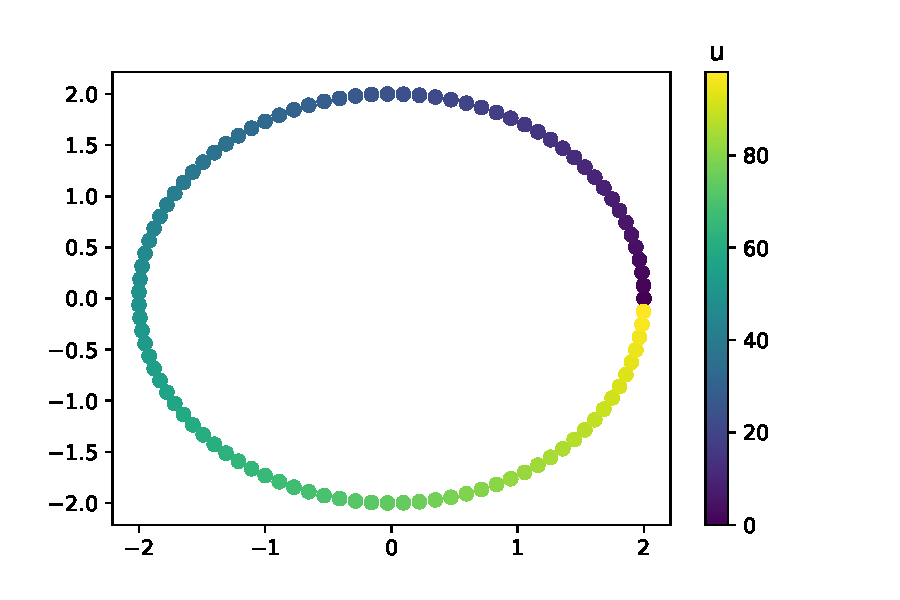
\includegraphics[width=\linewidth]{./images/initial_conditons.pdf}
\caption{Discrete nodes colored with their initial heat value prescribed by the boundary conditions.}
\label{fig::heat::initial}
\end{subfigure}
\hfill
\begin{subfigure}{.45\textwidth}
  \centering
  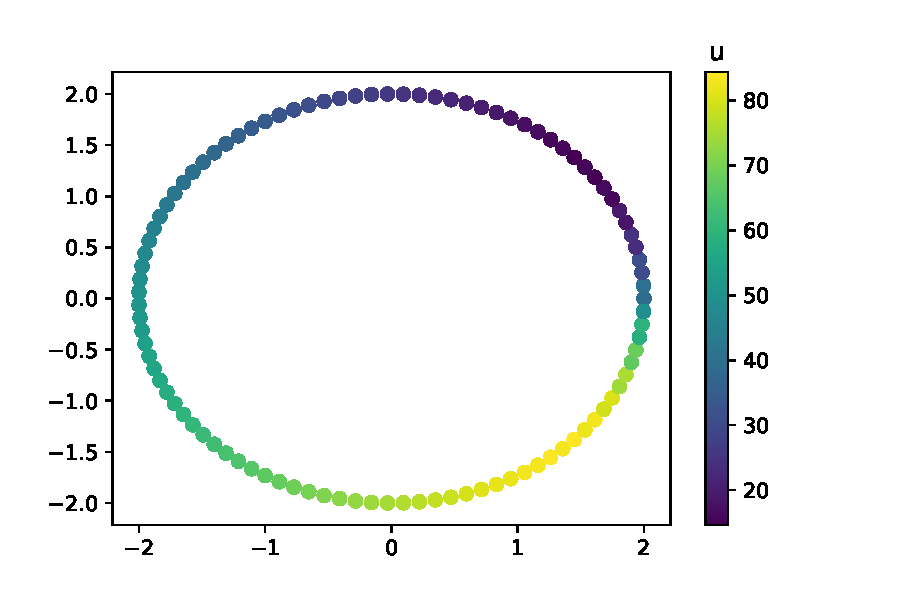
\includegraphics[width=\linewidth]{./images/solution.pdf}
\caption{Discrete nodes colored with final heat value at the final time $t=45$. }
\label{fig::heat:solution}
\end{subfigure}
\caption{The initial heat values prescribed by the boundary conditions~(\subref{fig::heat::initial}) and the final solution after 45 time steps~(\subref{fig::heat:solution}).}
\end{figure}


\begin{lstlisting}[language=c++,caption={Serial implementation of the one-dimensional heat equation \label{code:heat:central:difference}},float,floatplacement=tb]
struct stepper
{
    // Our partition type
    typedef double partition;

    // Our data for one time step
    typedef std::vector<partition> space;

    // Our operator
    static double heat(double left, double middle, double right)
    {
        return middle + (k*dt/(dx*dx)) * (left - 2*middle + right);
    }

    // do all the work on 'nx' data points for 'nt' time steps
    space do_work(std::size_t nx, std::size_t nt)
    {
        // U[t][i] is the state of position i at time t.
        std::vector<space> U(2);
        for (space& s : U)
            s.resize(nx);

        // Initial conditions: f(0, i) = i
        for (std::size_t i = 0; i != nx; ++i)
            U[0][i] = double(i);

        // Actual time step loop
        for (std::size_t t = 0; t != nt; ++t)
        {
            space const& current = U[t % 2];
            space& next = U[(t + 1) % 2];

            next[0] = heat(current[nx-1], current[0], current[1]);

            for (std::size_t i = 1; i != nx-1; ++i)
                next[i] = heat(current[i-1], current[i], current[i+1]);

            next[nx-1] = heat(current[nx-2], current[nx-1], current[0]);
        }

        // Return the solution at time-step 'nt'.
        return U[nt % 2];
    }
};
\end{lstlisting} 

%----------------------------------------------------------------------------------------
\subsection{Adding grain size control}
%----------------------------------------------------------------------------------------
In Figure~\ref{fig:hpx:stencil:scaling1} we have seen that we got some speedup with the asynchronous implementation discussed in Section~\ref{sec:hpx:advanced:sync}. However, in same cases the granularity (the amount of work) for each core was too small, since we always used one grid point wrapped in a future. Now, we want to extend the code to use partitions of grid nodes, see Figure~\ref{}. In this example we have a grid with nine nodes and we split them into three partitions, which means that each core has to compute the new values for three elements instead of for one element. The first, thing we need to do is to update the \cpp{struct participation}, see Listing~\ref{code:heat:garain:size}. In Line~4 a \cpp{std::vector<double>} is added to store the partition. In Line~8 a constructor is added to initialize the vector \cpp{data_(size)} with the provided \cpp{size_t size}. In Line~12 a second constructor is added to fill the partition with the initial values and the boundary values. Since the partition vector is declared as \cpp{private}, we use operator overloading in Line~21 and Line~25 to access the elements of the partition. For more details about operation overloading, see Section~\ref{sec:operator:overloading}. In Line~29 a function to obtain the partition size is added. \\

For the swapping scheme between the time steps for the computation of the temperature, see Figure~\ref{fig:heat:swap}, some small notification is applied as well. Figure~\ref{heat:swapping:partition} shows the principle of the swapping scheme using partitions. The fundamental principle is the same and we have the two space \cpp{U} to swap between the current time step and the future time step. However, with introducing the partitions, we have the two spaces per partition. These modifications are shown in Listing~\ref{code:heat:grain:size:stepper}. In Line~4 the \cpp{partition} is now of the type \cpp{partition_data}, see Listing~\ref{code:heat:garain:size}. In Line~10, each of the space vectors's size is set to the amount of partitions \cpp{np}. In Line~14, we access the space vector \cpp{U[0]} for the first time step and with \cpp{U[0][i]} each partition is accessed. We call the constructor for each partition and assign the initial values and boundary conditions. The full code is available on GitHub\link{https://github.com/STEllAR-GROUP/hpx/blob/master/examples/1d_stencil/1d_stencil_3.cpp}.


\begin{figure}[tp]
\centering
\begin{tikzpicture}

\foreach \i in {1,...,9}{
	\node at (\i,0) {\pgfuseplotmark{square*}};
}
\foreach \i in {1,...,9}{
	\node[below] at (\i,-0.1) {$x_\i$};	
}

\draw (1,-.6) -- (1,-1);
\draw (3.5,-.6) -- (3.5,-1);
\draw (6.5,-.6) -- (6.5,-1);
\draw (9,-.6) -- (9,-1);
\node[below] at (2.5,-1) {$n_1$};	
\node[below] at (5,-1) {$n_2$};	
\node[below] at (8,-1) {$n_3$};	
\end{tikzpicture}
\caption{Splitting the one-dimensional grid with nine grid nodes $(x_1,\ldots,x_9)$ into three partitions $(n_1,n_2,n3)$ to control the grain size.}
\end{figure}



\begin{lstlisting}[language=c++,caption={Serial implementation of the one-dimensional heat equation with grain size control. \label{code:heat:garain:size}},float,floatplacement=tbp]
struct partition_data
{


private:
    std::vector<double> data_;

public:

// Constructor
partition_data(std::size_t size = 0)
      : data_(size)
    {}

partition_data(std::size_t size, double int_value)
      : data_(size)
    {
        double base_value = 
              double(int_value * size);
        for (std::size_t i = 0; i != size; ++i)
            data_[i] = base_value + double(i);
    }

//Operator overloading 
double& operator[](std::size_t idx) { 
     return data_[idx]; 
  }
    
double operator[](std::size_t idx) const { 
       return data_[idx]; 
    }

// Util
std::size_t size() const { 
       return data_.size(); 
    }
};
\end{lstlisting}

\begin{figure}[tb]
\centering
\begin{tikzpicture}

\foreach \j in {0,...,1}{


\foreach \i in {1,...,4}{
	\node at (\j*5+\i,1.5) {\pgfuseplotmark{square*}};
}

\foreach \i in {1,...,4}{
	\node at (\j*5+\i,0.75) {\pgfuseplotmark{square*}};
}


\foreach \i in {1,...,4}{
	\node at (\j*5+\i,0) {\pgfuseplotmark{square*}};
}
\foreach \i in {1,...,4}{
	\node[below] at (\j*5+\i,-0.1) {$x_\i$};	
}

\node[left] at  (\j*5+0.5,0) {\small U[0][\j]};
\node[left] at  (\j*5+0.5,0.75) {\small U[1][\j]};
\node[left] at  (\j*5+0.5,1.5) {\small U[0][\j]};

\draw (\j*5+2,0) -- (\j*5+3,0.75);
\draw (\j*5+3,0) -- (\j*5+3,0.75);
\draw (\j*5+4,0) -- (\j*5+3,0.75);

\draw (\j*5+2,0.75) -- (\j*5+3,1.5);
\draw (\j*5+3,0.75) -- (\j*5+3,1.5);
\draw (\j*5+4,0.75) -- (\j*5+3,1.5);

} 

\node[right] at  (9.5,0) {t=1};
\node[right] at  (9.5,0.75) {t=2};
\node[right] at  (9.5,1.5) {t=3};

\end{tikzpicture}
\caption{Swapping between the partitions using the two spaces \cpp{U}. Note that each partition $n$ has his dedicated spaces, however, the fundamental principle stays the same.}
\label{heat:swapping:partition}
\end{figure}



\begin{lstlisting}[language=c++,caption={Serial implementation of the one-dimensional heat equation with grain size control. \label{code:heat:grain:size:stepper}},float,floatplacement=tbp]
class stepper
{
    // Our data for one time step
    typedef partition_data partition;
    typedef std::vector<partition> space;
    
    std::vector<space> U(2);
    for (space& s: U)
        // np is the number of partitions
        s.resize(np);
        
    // Initial conditions: f(0, i) = i
    for (std::size_t i = 0; i != np; ++i)
        U[0][i] = partition_data(nx, double(i));
        
    // Return the solution at time-step 'nt'.
    return U[nt % 2];
    
}
\end{lstlisting}


\newpage
\theendnotes

%----------------------------------------------------------------------------------------
\part{Parallel and distributed computing}
%----------------------------------------------------------------------------------------

%----------------------------------------------------------------------------------------
\chapter{Parallel computing}
%----------------------------------------------------------------------------------------
In this Chapter, a brief overview of the technical aspects of parallel computing is given. Note that this course focuses on the implementation details, like asynchronous programming, see Chapter~\ref{sec:async:coding}; parallel algorithms, see Section~\ref{sec:stl:parallel:algorithms}; and the C++ standard library for parallelism and concurrency (HPX), see Chapter~\ref{sec:hpx}. However, we provide some details and further references for the technical aspects and hardware details.\\

Let us begin with a definition of parallelism: \textit{1)} we need multiple resources which can operate at the same, \textit{2)} we have to have more than one task that can be performed at the same time, \textit{3)} we have to do multiple tasks on multiple resources the same time. First, we have to have multiple resources, \emph{e.g.}\ multiple threads of a computation node at the same time. However, with current hardware architecture this is not an issue. Second, this part is more interesting, since we need some code which is independent of each other and can be executed concurrent. Third, here we want to have overlapping computations and communication on multiple resources. For more details about parallel computing, we refer to~\cite{grama2003introduction,trobec2018introduction}.\\

For the second part of the definition, Amdahl's law\index{Amdahl's law}~\cite{amdahl1967validity} or strong scaling\index{scaling} is important. Amdahl's law is given as
\begin{align}
S = \frac{1}{(1-P) + \frac{P}{N}}
\end{align}
where $S$ is the speed up, $P$ the proportion of parallel code, and $N$ the numbers of threads. Figure~\ref{fig:amdals:law} plots Amdahl's law for different ratios of parallel code. Obviously, for zero percent parallel code, there is no speedup. If the portion to parallel code increases, the speedup increases up to a certain amount of threads. Therefore, the parallel computing with many threads is only beneficial for highly parallelism in our program. For example if our code took 20 hours using a single thread to complete and there in a part of one hour which can not be executed in parallel. Thus, only 19 hours of execution time can be parallized $(p=0.95)$ and independent of the amount of threads we use the theoretical speedup is limited to $S=\sfrac{1}{(1-p)}=20$.\\

\begin{figure}[tb]
\centering
 \begin{tikzpicture}
        \begin{axis}[
            no markers,
            samples=100,
            /pgf/declare function={
            f(\x,\a) = 1. / ((1.-\a)+(\a/x));
       		},
       		grid=both,
       		xlabel=$N$ number of threads,
       		ylabel=$S$ speedup,
       		legend pos=outer north east,
        ]
            % ... and use it here
            \addplot+ [domain=1:2048,azure,thick] {f(x,0)};
            \addlegendentry{$P=0\%$}
            \addplot+ [domain=1:2048,cadetgrey,thick] {f(x,0.5)};
            \addlegendentry{$P=50\%$}
            \addplot+ [domain=1:2048,darkgreen,thick] {f(x,.75)};
            \addlegendentry{$P=75\%$}
            \addplot+ [domain=1:2048,amaranth,thick] {f(x,.90)};
            \addlegendentry{$P=90\%$}
            \addplot+ [domain=1:2048,black,thick] {f(x,.95)};
            \addlegendentry{$P=95\%$}
       \end{axis}
    \end{tikzpicture}
\caption{Plot of Amdahl's law for different parallel portions of the code.}
\label{fig:amdals:law}
\end{figure}

Before we look into different parallelism approaches, we look into the example how to compute the dot product $S = \mathbf{X} \cdot \mathbf{V} = \sum_i^N x_i y_i$ of two vectors $\mathbf{X} = \lbrace x_1,x_2,\ldots,x_n \rbrace$ and $\mathbf{Y} = \lbrace y_1,y_2,\ldots,y_n \rbrace$  in a sequential manner and extend this example to the various parallelism approaches. So we have to compute $S = (x_1y_1) + (x_2y_2) + \ldots + (x_n y_n)$ as shown in the flow chart in Figure~\ref{fig:flow:chart:dot:seq}. In the sequential processing, the first to elements of each vector are multiplied $x_1 \times y_1$ and added to the temporal result. After that the second elements are multiplied and added to the temporal result, and so on. \\

\begin{figure}
\centering
\begin{tikzpicture}
\draw (0,0) circle [radius=0.3] node {$\times$};
\draw (2,0) circle [radius=0.3] node {$\times$};
\draw (4,0) circle [radius=0.3] node {$\times$};
\draw (6,0) circle [radius=0.3] node {$\times$};
\draw (10,0) circle [radius=0.3] node {$\times$};
\node[above] at (8,0) {$\ldots$} ;

\draw (2,-1) circle [radius=0.3] node {$+$};
\draw (4,-1) circle [radius=0.3] node {$+$};
\draw (6,-1) circle [radius=0.3] node {$+$};
\draw (10,-1) circle [radius=0.3] node {$+$};
\node[above] at (8,-1) {$\ldots$} ;

\draw[->](0,-0.3) -- (1.7,-1);
\draw[->](2,-0.3) -- (2,-0.7);
\draw[->](4,-0.3) -- (4,-0.7);
\draw[->](6,-0.3) -- (6,-0.7);
\draw[->](10,-0.3) -- (10,-0.7);

\draw[->](2.3,-1) -- (3.7,-1.);
\draw[->](4.3,-1) -- (5.7,-1.);
\draw[->](6.3,-1) -- (7.7,-1.);
\draw[->](8.3,-1) -- (9.7,-1.);

\draw (-0.15,0.3) -- (-0.3,0.6);
\node[above] at (-0.3,0.6) {$x_1$} ;
\draw (2-0.15,0.3) -- (2-0.3,0.6);
\node[above] at (2-0.3,0.6) {$x_2$} ;
\draw (4-0.15,0.3) -- (4-0.3,0.6);
\node[above] at (4-0.3,0.6) {$x_3$} ;
\draw (6-0.15,0.3) -- (6-0.3,0.6);
\node[above] at (6-0.3,0.6) {$x_4$} ;
\draw (10-0.15,0.3) -- (10-0.3,0.6);
\node[above] at (10-0.3,0.6) {$x_n$} ;

\draw (0.15,0.3) -- (0.3,0.6);
\node[above] at (0.3,0.6) {$y_1$} ;
\draw (2+0.15,0.3) -- (2+0.3,0.6);
\node[above] at (2+0.3,0.6) {$y_2$} ;
\draw (4+0.15,0.3) -- (4+0.3,0.6);
\node[above] at (4+0.3,0.6) {$y_3$} ;
\draw (6+0.15,0.3) -- (6+0.3,0.6);
\node[above] at (6+0.3,0.6) {$y_4$} ;
\draw (10+0.15,0.3) -- (10+0.3,0.6);
\node[above] at (10+0.3,0.6) {$y_n$} ;

\draw[->](10,-1.3) -- (10,-1.6);
\node[below] at (10,-1.6) {$s$} ;
\end{tikzpicture}
\caption{Flow chart of the sequential evaluation of the dot product of two vectors. }
\label{fig:flow:chart:dot:seq}
\end{figure}

The first parallelism approach is the pipeline parallelism\index{pipeline parallelism}~\cite{ramamoorthy1977pipeline}. The pipeline parallelism is used in vector processors and in execution pipelines in all general microprocessors. Let us look into some example of from the automotive industry. First, the body of the car is assembled. Second, workers assemble the chassis. Third, workers add the engine into the chassis. Next, the steering wheel is added and many more steps until the car is finally assembled. TO make this process efficient, the workers assembling the chassis do not wait until the last step is finalized before they start working on the next chassis. Side note this is similar to the assembly line introduced bu Henry Ford to enable mass production of cars~\cite{watts2009people}.\\

Figure~\ref{fig:dataflow:pipeline} shows the data flow chart for the pipeline parallelism. In the first step, the values $x_1$ and $y_1$ are read from memory. In the second step the values are multiplied. In the last step the result of the multiplication is added to the variable $S$. However, the other threads do not idle until the result is computed and do a previous step if possible. Meaning if the multiplication at stage two is happening, another thread starts to get the next values. For more details, we refer to~\cite{quinn2003parallel}. \\


\begin{figure}[tb]
\centering
\begin{tikzpicture}
\draw (0,0) rectangle ++(0.75,0.75) node[pos=.5] {$+S$};
\draw (1.5,0) rectangle ++(0.75,0.75) node[pos=.5] {$xy$}; 
\draw (3.5,0) rectangle ++(2,0.75) node[pos=.5] {\text{get} $x_i$,$y_i$};

\node[above] at (8,0.5*0.75) {$\mathbf{X} = \lbrace x_1,x_2,\ldots,x_n \rbrace$} ;
\node[below] at (8,0.5*0.75) {$\mathbf{Y} = \lbrace y_1,y_2,\ldots,y_n \rbrace$} ;
\node at (-1,0.5*0.75) {$S$} ;

\draw[<-](-0.8,0.5*0.75) -- (0,0.5*0.75) ;
\draw[<-](0.75,0.5*0.75) -- (1.5,0.5*0.75) ;
\draw[<-](2.25,0.5*0.75) -- (3.5,0.5*0.75) ;
\draw[<-](5.75,0.8*0.75) -- (6,0.8*0.75) ;
\draw[<-](5.75,0.2*0.75) -- (6,0.2*0.75) ;
\end{tikzpicture}
\caption{Flow chart for the pipeline processing for the dot product.}
\label{fig:dataflow:pipeline}
\end{figure}

The second parallelism approach is the Single instructions and multiple data (SIMD)\index{SIMD}\index{single instructions and multiple data}. SIMD is part of Flynn's taxonomy, a classification of computer architectures, proposed by Michael J. Flynn in 1966~\cite{flynn1972some,duncan1990survey}. Following aspects are relevant 
\begin{itemize}
\item All perform same operation at the same time
\item But may perform different operations at different times
\item Each operates on separate data
\item Used in accelerators on microprocessors
\item Scales as long as data scales.
\end{itemize}
\vspace{0.25cm}
Figure~\ref{fig:reduction:tree:simd} shows the reduction tree for the dot product computation. For this parallelism approach all threads perform the same operation at the same time. In our case all available threads multiply two values at the first level. Second one of these threads add the partial results. Until not all elements are read from the vector these steps are repeated. The last step is to accumulate all partial results and the final result is available. For example previous CUDA architectures were designed this way and introducing branching had some effect on the performance. Newer CUDA architectures perform better here and these things are explained in following talk\link{https://youtu.be/5vr7ItjyIH8}.

\begin{figure}[tb]
\centering
  \begin{tikzpicture}
   \draw (0,0) rectangle ++(0.75,0.75) node[pos=.5] {$P_1$}; 
   \draw (1.5,0) rectangle ++(0.75,0.75) node[pos=.5] {$P_2$}; 
   \draw (3,0) rectangle ++(0.75,0.75) node[pos=.5] {$P_3$}; 
   \draw (4.5,0) rectangle ++(0.75,0.75) node[pos=.5] {$P_4$}; 
   
   \draw (0.75,-2) rectangle ++(0.75,0.75) node[pos=.5] {$+$}; 
   \draw (3.75,-2) rectangle ++(0.75,0.75) node[pos=.5] {$+$}; 
   
   \draw (2.25,-4) rectangle ++(0.75,0.75) node[pos=.5] {$+$}; 
   
   \draw[->] (0.75+0.5*0.75,-2) -- (2.25,-4+0.75) ;
   \draw[->] (3.75+0.5*0.75,-2) -- (3,-4+0.75) ;
   
   \draw[->] (1.5+0.5*0.75,0) -- (1.5,-2+0.75) ;
   \draw[->] (0.5*0.75,0) -- (0.75,-2+0.75) ; 
   
   \draw[->] (3+0.5*0.75,0) -- (3.75,-2+0.75) ;
   \draw[->] (4.5+0.5*0.75,0) -- (4.5,-2+0.75) ; 
   
   \draw[->] (2.25+0.5*0.75,-4) -- (2.25+0.5*0.75,-4.5) ; 
   
   \draw[dashed] (0,-0.75) -- (5,-0.75) ;
   \node[below,rotate=90] at (-.75,-2) {\small Reduction tree}; 
   
   \node at (0.5*0.75,1.5) {\tiny $X=\lbrace x_1,x_2 \rbrace$};
   \node at (0.5*0.75,1.25) {\tiny $Y=\lbrace x_9,x_{10} \rbrace$};
   \node at (1.5+0.5*0.75,1.5) {\tiny $X=\lbrace x_3,x_4 \rbrace$};
   \node at (1.5+0.5*0.75,1.25) {\tiny $Y=\lbrace x_{11},x_{12} \rbrace$};
   \node at (3.+0.5*0.75,1.5) {\tiny $X=\lbrace x_5,x_6 \rbrace$};
   \node at (3.+0.5*0.75,1.25) {\tiny $Y=\lbrace x_{13},x_{14} \rbrace$}; 
   \node at (4.5+0.5*0.75,1.5) {\tiny $X=\lbrace x_7,x_8 \rbrace$};
   \node at (4.5+0.5*0.75,1.25) {\tiny $Y=\lbrace x_{15},x_{16} \rbrace$};
   
   \draw[->] (0.5*0.75,1.125) -- (0.5*0.75,0.75) ;
   \draw[->] (1.5+0.5*0.75,1.125) -- (1.5+0.5*0.75,0.75) ;
   \draw[->] (3.+0.5*0.75,1.125) -- (3.+0.5*0.75,0.75) ;
   \draw[->] (4.5+0.5*0.75,1.125) -- (4.5+0.5*0.75,0.75) ;
   \end{tikzpicture}
   \caption{Reduction tree for the dot product using single instructions and multiple data.}
   \label{fig:reduction:tree:simd}
\end{figure}

%----------------------------------------------------------------------------------------
\subsection*{Memory access}
\index{memory access}
%----------------------------------------------------------------------------------------
For parallel computing, the memory access scheme is important to understand performance behavior. If we initialize for example the two vectors in the dot product example, some space in the memory is reserved and filled with the values. For the computation of the dot product these elements have to be read from memory and the CPU is doing the computation. In a layman's view the CPU is connected to the memory via a so-called bus. Depending on the bus's architecture the access time differs and may have effects on the performance if there is a switch from one CPU to the second CPU.\\

The first memory access scheme is uniform memory access (UMA), see Figure~ref{fig:memory:uma},  where all memory is attached to one bus and all CPU are attached to the same bus. Therefore, the memory access times are the same for all CPU. So we do not see any effect if we switch from one two two CPU. The second memory access scheme is non-uniform memory access (NUMA), see Figure~\ref{fig:memory:numa}. Here, the access time to the memory depends on the memory location relative to the CPU. Thus, local memory access is fast and non-local memory access has some overhead. For more details about memory access, we refer to~\cite{el2005advanced,hager2010introduction}.

\begin{figure}
\centering
\begin{minipage}[c]{0.45\textwidth}
\centering
   \begin{tikzpicture}
%Threads
\draw (0,3) rectangle (.5,3.5) node[pos=.5] {1};
\draw (0.5,3) rectangle (1.0,3.5) node[pos=.5] {..};
\draw (1.,3) rectangle (1.5,3.5) node[pos=.5] {n};

\draw (2.5,3) rectangle (3.,3.5) node[pos=.5] {1};
\draw (3.,3) rectangle (3.5,3.5) node[pos=.5] {..};
\draw (3.5,3) rectangle (4,3.5) node[pos=.5] {n};

\draw (0.75,2.5) -- (0.75,3.);
\draw (3.25,2.5) -- (3.25,3.);

%BUS
\draw (0,1) rectangle (4,1.5) node[pos=.5] {Bus};


%CPU
\draw (0,2) rectangle (1.5,2.5) node[pos=.5] {CPU 1};
\draw (2.5,2) rectangle (4,2.5) node[pos=.5] {CPU 2};
\draw (0.75,2) -- (0.75,1.5);
\draw (3.25,2) -- (3.25,1.5);

%Memory
\draw (0,0) rectangle (4,0.5) node[pos=.5] {Memory};
\draw (0.75,.5) -- (0.75,1.);
\draw (3.25,.5) -- (3.25,1.);
\end{tikzpicture}
    \caption{Uniform memory access (UMA)\index{uniform memory access}\index{UMA}}
    \label{fig:memory:uma}
\end{minipage}
\hfill
\begin{minipage}[c]{0.45\textwidth}
\begin{tikzpicture}
%Threads
\draw (0,3) rectangle (.5,3.5) node[pos=.5] {1};
\draw (0.5,3) rectangle (1.0,3.5) node[pos=.5] {..};
\draw (1.,3) rectangle (1.5,3.5) node[pos=.5] {n};

\draw (2.5,3) rectangle (3.,3.5) node[pos=.5] {1};
\draw (3.,3) rectangle (3.5,3.5) node[pos=.5] {..};
\draw (3.5,3) rectangle (4,3.5) node[pos=.5] {n};

\draw (0.75,2.5) -- (0.75,3.);
\draw (3.25,2.5) -- (3.25,3.);

%BUS
\draw (0,1) rectangle (1.5,1.5) node[pos=.5] {Bus};
\draw (2.5,1) rectangle (4,1.5) node[pos=.5] {Bus};

%CPU
\draw (0,2) rectangle (1.5,2.5) node[pos=.5] {CPU 1};
\draw (2.5,2) rectangle (4,2.5) node[pos=.5] {CPU 2};
\draw (0.75,2) -- (0.75,1.5);
\draw (3.25,2) -- (3.25,1.5);

%Memory
\draw (0,0) rectangle (1.5,0.5) node[pos=.5] {Memory};
\draw (2.5,0) rectangle (4,0.5) node[pos=.5] {Memory};
\draw (0.75,.5) -- (0.75,1.);
\draw (3.25,.5) -- (3.25,1.);
\end{tikzpicture}
    \caption{Non-uniform memory access (NUMA)\index{non-uniform memory access}\index{NUMA}}
    \label{fig:memory:numa}
\end{minipage}

\end{figure}



%----------------------------------------------------------------------------------------
\section{Caution: Data races and dead locks}
\label{sec:deadlocks}
%----------------------------------------------------------------------------------------
Remember with great power comes great responsibility! Meaning with shared memory parallelism you add an additional source of error to your code. When using parallel execution policy, it is the programmer's responsibility to avoid
\begin{itemize}
\item data races
\item race conditions
\item deadlocks.
\end{itemize} 
Let us look into some code examples for these kind of errors. A data race\index{data race} exists when multithreaded (or otherwise parallel) code that would access a shared resource could do so in such a way as to cause unexpected results. Listing~\ref{code:data:race} shows an example for a data race for the variable \cpp{sum}. Since the parallel execution policy is used, multiple threads can access the variable \cpp{sum} at the same time which means that not all threads can write to the variable. Thus, the result is might not correct. There are two solutions to avoid the data race. First, the atomic library\link{https://en.cppreference.com/w/cpp/atomic/atomic}. The atomic library\footnote{\tiny\url{https://en.cppreference.com/w/cpp/atomic}} provides components for fine-grained atomic operations allowing for lockless concurrent programming. Each atomic operation is indivisible with regards to any other atomic operation that involves the same object. Atomic objects are free of data races. Listing~\ref{code:datarace:atomic} shows the solution using \cpp{std::atomic:<int>}\link{https://en.cppreference.com/w/cpp/atomic/atomic}. The second solution is shown in Listing~\ref{code:datarace:mutex}. Here, the \cpp{std::mutex} class is used to avoid the data race. The mutex class\link{https://en.cppreference.com/w/cpp/thread/mutex} is a synchronization primitive that can be used to protect shared data from being simultaneously accessed by multiple threads. In Line~4 a \cpp{std::mutex m;} is generated. In Line~8 the lock of the code is started by using \cpp{m.lock();} and in Line~10 the lock is released by using \cpp{m.unlock();}.

\begin{exercise}
Give a definition for \cpp{std::atomic} and \cpp{std::mutex} in your own words. 
\end{exercise}

Another source of error is the race condition\index{race condition} where a check of a shared variable within a parallel execution and another thread could change this variable before it is used. Listing~\ref{code:racecondition} shows the solution to avoid the race condition.  Imagine the code without the \cpp{std::mutex} and the implication to get a wrong result. In the code there is a check if \cpp{x} is equal to 5 and a special treatment of the computation in this case. Now in Line~4 it was true that \cpp{x} was equal to five and the thread enters the \cpp{if} branch. However, in between another thread could change the value of \cpp{x} and not \cpp{y = 5 *2} is computed. By using the mutex this situation is avoided.

\begin{exercise}
Explain a data race in your own words and explain why a \cpp{std::mutex} avoids the data race.
\end{exercise}

\begin{lstlisting}[language=c++,caption={Example code and Solution for a data race.\label{code:data:race}},float,floatplacement=tb]
//Compute the sum of the array a in parallel
int a[] = {0,1,2,3,4};
int sum = 0;
std::for_each(std::execution::par, 
              std::begin(a), 
              std::end(a), [&](int i) {
  sum += a[i]; // Error: Data race
});
\end{lstlisting}


\begin{lstlisting}[language=c++,caption={Solution to avoid the data race using \cpp{std::atomic}.\label{code:datarace:atomic}},float,floatplacement=tb]
//Compute the sum of the array a in parallel
int a[] = {0,1};
std::atomic<int> sum{0};
std::for_each(std::execution::par, 
              std::begin(a), 
              std::end(a), [&](int i) {
  sum += a[i]; 
});
\end{lstlisting}

\begin{lstlisting}[language=c++,caption={Solution to avoid the data race using \cpp{std::mutex}.\label{code:datarace:mutex}},float,floatplacement=tb]
//Compute the sum of the array a in parallel
int a[] = {0,1};
int sum = 0;
std::mutex m;
std::for_each(std::execution::par, 
              std::begin(a), 
              std::end(a), [&](int i) {
  m.lock();
  sum += a[i];
  m.unlock(); 
});
\end{lstlisting}


\begin{lstlisting}[language=c++,caption={Example for the race condition.\label{code:racecondition}},float,floatplacement=tb]
std::mutex m;

m.lock();
if (x == 5)  // Checking x
{
   // Different thread could change x 
      
   y = x * 2; // Using x
}
m.unlock();
// Now it is sure that y will be 10
\end{lstlisting}


A deadlock\index{deadlock} describes a situation where two or more threads are blocked forever and waiting for each others. Following example taken from\link{https://docs.oracle.com/javase/tutorial/essential/concurrency/deadlock.html} explains a deadlock nicely. \\

\textit{Alphonse and Gaston are friends, and great believers in courtesy. A strict rule of courtesy is that when you bow to a friend, you must remain bowed until your friend has a chance to return the bow. Unfortunately, this rule does not account for the possibility that two friends might bow to each other at the same time.}

\begin{exercise}
The implementation of this examples is available on GitHub\link{https://github.com/diehlpkteaching/ParallelComputationMathExamples/blob/master/chapter10/lecture6-deadlock.cpp.ipynb}. Play around with the example and try to understand why the code results in a deadlock. 
\end{exercise}

%----------------------------------------------------------------------------------------
\chapter{Asynchronous programming}
\label{sec:async:coding}
\index{future}
\index{async}
\index{C++!asynchronous programming}
%----------------------------------------------------------------------------------------
A different concept for shared memory parallelism is asynchronous programming~\cite{williams2012c++}. Before we look into asynchronous programming, we look again into the concept of serial programming. Figure~\ref{fig:async:dependencygraph} shows the dependency graph for one computation and one can see that we can compute $P$ and $X$ independent and only $H$ depends on both of them. Listing~\ref{code:serial:dependency} shows the serial computation of the dependency graph. Each line of code is executed line by line Each time a function is called the code waits until the function finishes. Thus, we can not compute $P$ and $X$ independently, even if the data is independent. 

\vspace{0.25cm}
\begin{minipage}{\linewidth}
\begin{minipage}{0.45\linewidth}
\centering
\begin{tikzpicture}
\node (a) [draw,circle] at (0,2) {$H$};
\node (b) [draw,circle] at (0,0) {$P$};
\node (c) [draw,circle] at (1,0) {$X$};
\draw [->] (a) -- (b);
\draw [->] (a) -- (c);
\end{tikzpicture}
\captionof{figure}{Example dependency graph}
\label{fig:async:dependencygraph}
\end{minipage}
\hfill
\begin{minipage}{0.5\linewidth}
\begin{lstlisting}[language=c++,caption={Synchronous execution of the dependency graph.\label{code:serial:dependency}}]
auto P = compute();
auto X = compute();
auto H = compute(P,X);
\end{lstlisting}
\end{minipage}
\end{minipage}
\vspace{0.25cm}

To executed lines asynchronously the C++ language provides the \cpp{std::async}\link{https://en.cppreference.com/w/cpp/thread/async}\index{async}\index{C++!async} expression provided by the \cpp{#include <future>}. Listing~\ref{code:async:dependency} shows the asynchronous implementation of the dependency graph in Figure~\ref{fig:async:dependencygraph}. Line~2 shows the usage of \cpp{std::async} for the function \cpp{compute}. The first argument is the name of the function or a lambda expression, see Section~\ref{sec:lambda:function}. Because we used \cpp{std::async} this line of code is executed in the background on a different thread and the next line of code is executed, even if the result of the computation is not ready yet. Therefore, \cpp{std::async} return a \cpp{std::future<int>}\link{https://en.cppreference.com/w/cpp/thread/future}\index{future}\index{C++!future} object provided by the \cpp{#include <future>} header which is a template and contains the return type of the function which is in this example the \cpp{int} data type. In Line~4, the computation of $X$ is started on another thread. Such that both computations happens at the same time. In Line~7--9 the results of the asynchronous function call are gathered, since these are needed to compute $H$. With the \cpp{.get()} function a barrier is introduced and the line of codes waits until the computation is ready. In our case, we can wait since we need the two results to compute the last one. Meaning that Line~8 is only executed if the computation in Line~2 has finished. Following synchronization features are available:
\begin{itemize}
\item \lstinline|.get()| returns the result of the functions and wait until the computation finished
\item \lstinline|.wait()|\link{https://en.cppreference.com/w/cpp/thread/future/wait} waits until the computation finished
\item \lstinline|.wait_for(std::chrono::seconds(1))|\link{https://en.cppreference.com/w/cpp/thread/future/wait_for} returns if it is not available for the specified timeout duration 
\item \lstinline|.wait_until(std::chrono::seconds(1))|\link{https://en.cppreference.com/w/cpp/thread/future/wait_until} waits for a result to become available. It blocks until specified timeout time has been reached or the result becomes available, whichever comes first. 
\end{itemize}

\begin{lstlisting}[language=c++,caption={Asynchronous execution of the dependency graph.\label{code:async:dependency}},float,floatplacement=tb]
// Compute P
std::future<int> f1 = std::async(compute);
// Compute X
auto f2 = std::async(compute);

// Gather the results
int P = f1.get();
int X = f2.get();

// Compute the dependent result H
std::cout << compute(P,X) << std::endl;
\end{lstlisting}

\section*{Example}
Let us look into one example to show the parallelism using asynchronous programming for the Taylor series. The approximation of the $\sin$ function is given as
\begin{align}
\sin(x) = \sum\limits_{n=0}^N (-1)^{n-1} \frac{x^{2n}}{(2n)!} 
\label{eq:sin:taylor}
\end{align}
One approach to parallize the above function using two threads is:
\begin{enumerate}
\item Split $n$ into slices, e.g. 2 times $\sfrac{n}{2}$ for two threads
\item Start two times \lstinline|std::async| where each thread computes $\sfrac{n}{2}$
\item Use the two futures to synchronize the results
\item Combine the two futures to obtain the result.
\end{enumerate}
To distribute $n$ into slices, we need to write the sum in Equation~\eqref{eq:sin:taylor} as
\begin{align}
\sum\limits_{n=begin}^{end} (-1)^{n-1} \frac{x^{2n}}{(2n)!} \text{.}
\end{align}
Listing~\ref{code:async:taylor} shows how to implement the function to splice the computation of the Taylor series, see Line~5--14. In Line~18--19 the two splices $\sfrac{n}{2}$ are launched from $0$ up to $49$ on the first thread and from $50$ up to $99$ on the second thread. In Line~22 the result is gathered and finally the accumulated result is evaluated. For more details, we refer to following talk\link{https://www.youtube.com/watch?v=js-e8xAMd1s}.

To compile the code using asynchronous programming, we need to add \lstinline|-pthread| to our compiler to use the POSIX threads to launch the functions asynchronous (\lstinline|std::async|). More details about POSIX\index{POSIX} threads~\cite{butenhof1997programming,kleiman1996programming}.




\begin{lstlisting}[language=c++,caption={Asynchronous computation of the $\sin$ function using a Taylor series.\label{code:async:taylor}},float,floatplacement=tb]
#include <future>
#include <iostream>

// Function to compute portion of the Taylor series
double taylor(size_t begin, size_t end, 
double x,size_t n){
double res = 0;

	for( size_t i = begin ; i < end ; i++)
	{
	  res += pow(-1,i-1) * pow(x,2*n) / factorial(2*n);
	} 
return res;
}

int main(){
	// Asynchronous computation using two slices
	auto f1 = std::async(taylor,0,49,2,100); 
	auto f2 = std::async(taylor,50,99,2,100); 
	
	// Gather the result
	double result = f1.get() + f2.get();

	// Print the result
	std::cout << "sin(2)= " res << std::endl;

	return 0;
}
\end{lstlisting}


%----------------------------------------------------------------------------------------
\chapter{Distributed Programming}
%----------------------------------------------------------------------------------------
Previously, we considered shared memory parallelism which means we only considered one physical computational node. Now, we will look into distributed programming because the memory or the computational resources of one physical computational node are not sufficient. Figure~\ref{}



\newpage
\theendnotes


%----------------------------------------------------------------------------------------
\part{HPX}
\label{sec:hpx}
%----------------------------------------------------------------------------------------

%----------------------------------------------------------------------------------------
\chapter{Introduction to HPX}
%----------------------------------------------------------------------------------------
HPX (High Performance ParalleX) is a general purpose C++ runtime system for parallel and distributed applications of any scale. It strives to provide a unified programming model which transparently utilizes the available resources to achieve unprecedented levels of scalability.  This library strictly adheres to the C++14 Standard and leverages the Boost C++ Libraries which makes HPX easy to use, highly optimized, and very portable. These are the most notable features of HPX:
\vspace{0.25cm}
\begin{itemize}
\item HPX exposes a uniform, standards-oriented API for ease of programming parallel and \textcolor{azure}{distributed} applications.
\item HPX provides unified syntax and semantics for \textcolor{azure}{local and remote} operations.
\item HPX exposes a uniform, flexible, and extendable \textcolor{azure}{performance counter framework}~\cite{grubel2016dynamic,grubel2016using} which can enable runtime adaptivity
\item HPX has been designed and developed for systems of \textcolor{azure}{any scale}, from hand-held devices to very large scale systems (Raspberry Pi, Android, Server, up to super computers~\cite{daiss2019piz,heller2019harnessing}).
\end{itemize}
\vspace{0.25cm}
For a brief overview of HPX, we refer to~\cite{heller2017hpx} and for a detailed overview, we refer to~\cite{heller2019extending}. For more details about asynchronous many-task systems (AMT), we refer to~\cite{thoman2018taxonomy}.

%----------------------------------------------------------------------------------------
\subsection{Using HPX}
\label{sec:hpx:using}
%----------------------------------------------------------------------------------------
Let us look into HPX's hello world example. We have to ways to initialize the HPX runtime system. First way is to include the header \cpp{#include <hpx/hpx_main.hpp>}, see Listing~\ref{code:hpx:main}. In that case, the only thing we have to add is the new header file. Note that this header file should be the first one to be included. Before we can call the first HPX function, the HPX runtime system needs to be initialized. Second way is to include the header \cpp{#include <hpx/hpx_init.hpp>}, see Listing~\ref{code:hpx:init}. In that case, the \cpp{hpx_main} function is defined in Line~4 and we place the code as we like to have in the \cpp{main} function there and use \cpp{hpx::finalize()} as the return value to make sure the HPX runtime system is stopped. To initialize the HPX runtime system, the function \cpp{hpx::init(argc, argv)} has to be called. Note that this header file should be the first one to be included. All HPX functions have to be called within the \cpp{hpx_main} function to make sure the HPX runtime system is initialized. \\

Assuming that HPX is installed on the system, we need to provide some compiler and linker flags to compile the HPX application. Note that on Fedora one can install HPX by using \bash{sudo dnf install hpx-devel} or using this
tutorial\link{https://www.diehlpk.de/blog/hpx-fedora/}. Listing~\ref{code:cmake:hpx} shows a example \textit{CMakeLists.txt} file to compile the programs shown in Listing~\ref{code:hpx:main} or Listing~\ref{code:hpx:init}. For more details about CMake, we refer to Section~\ref{sec:cmake}. Listing~\ref{code:cmake:compile:hpx} shows how to compile the program and run it. Note that the command line option \cpp{--hpx:threads} specifies how many CPUs HPX is allowed yo use. 


\begin{lstlisting}[language=c++,caption={Initializing the HPX runtime system (I).\label{code:hpx:main}},float,floatplacement=tb]
#include <hpx/hpx_main.hpp>
#include <iostream>

int main()
{
    std::cout << "Hello World!\n" << std::endl;
    return 0;
}
\end{lstlisting}


\begin{lstlisting}[language=c++,caption={Initializing the HPX runtime system (II).\label{code:hpx:init}},float,floatplacement=tb]
#include <hpx/hpx_init.hpp>
#include <iostream>

int hpx_main(int, char**)
{
    // Say hello to the world!
    std::cout << "Hello World!\n" << std::endl;
    return hpx::finalize();
}

int main(int argc, char* argv[])
{
    return hpx::init(argc, argv);
}
\end{lstlisting}


\begin{minipage}{\linewidth}
\begin{minipage}{0.45\linewidth}
\begin{lstlisting}[language=bash,caption={Content of the CMakeLists.txt to build HPX applications.\label{code:cmake:hpx}},emph={project, add_executable,cmake_minimum_required},emphstyle={\color{azure}\bfseries}]
cmake_minimum_required(VERSION 3.3.2)
project(my_hpx_project CXX)
find_package(HPX REQUIRED)
add_hpx_executable(my_hpx_program
    SOURCES main.cpp
)
\end{lstlisting}
\end{minipage}
\hfill
\begin{minipage}{0.45\linewidth}
\begin{lstlisting}[language=bash,caption={Build instructions for CMake.\label{code:cmake:compile:hpx}}]
cmake .
make
./my_hpx_program --hpx:threads=4
\end{lstlisting}
\end{minipage}
\end{minipage}



%----------------------------------------------------------------------------------------
\section{Parallel algorithms}
\index{algorithms!parallel}
\index{parallel algorithms}
\index{HPX!parallel algorithms}
%----------------------------------------------------------------------------------------
In Section~\ref{sec:stl:parallel:algorithms} we looked at the experimental parallel algorithms provided by the C++ STL. HPX provides the parallel algorithms as well and the API is identical and we just need to replace the \cpp{std} name space with \cpp{hpx} name space. Recall the example in Listing~\ref{code:parallel:algorithms} and now we implement the same example using HPX's parallel algorithms. Listing~\ref{code:hpx:parallel:reduce} shows how to compute the sum of the elements in the vector \cpp{values} parallel. Note that solely had to replace \cpp{std::execution::par} by HPX's name space which is a little bit different and reads as \cpp{hpx::parallel::execution::par}. The same for \cpp{std::reduce} and this name space reads as \cpp{hpx::parallel::v1::reduce}\link{https://hpx-docs.stellar-group.org/latest/html/libs/algorithms/api.html?highlight=reduce\#\_CPPv3N3hpx8parallel2v16reduceERR8ExPolicy8FwdIterB8FwdIterE1TRR1F}. Until now the API is equal to the one of the C++ STL. Now, we look into the additional features provided by HPX. First, we look into the additional features for execution policies\index{HPX!execution policies}. In Line~16 we specify a dynamic chunk size \cpp{dynamic_chunk_size} and pass this execution policy to the execution policy using \cpp{.with(scs)}. Following execution parameters are provided:
\vspace{0.25cm}
\begin{itemize}
\item \lstinline|hpx::parallel::execution::static_chunk_size|\link{https://hpx-docs.stellar-group.org/latest/html/libs/execution/api.html?highlight=static\_chunk\_size\#\_CPPv3N3hpx8parallel9execution17static\_chunk\_sizeE} \\
Loop iterations are divided into pieces of a given size and then assigned to threads.
\item \lstinline|hpx::parallel::execution::auto_chunk_size|\link{https://hpx-docs.stellar-group.org/latest/html/libs/execution/api.html?highlight=auto\_chunk\_size\#\_CPPv3N3hpx8parallel9execution15auto\_chunk\_sizeE} \\
Pieces are determined based on the first 1\% of the total loop iterations. 
\item \lstinline|hpx::parallel::execution::dynamic_chunk_size|\link{https://hpx-docs.stellar-group.org/latest/html/libs/execution/api.html?highlight=dynamic\_chunk\_size\#\_CPPv3N3hpx8parallel9execution18dynamic\_chunk\_sizeE} \\
Dynamically scheduled among the cores and if one core finished it gets dynamically assigned a new chunk.
\end{itemize}
\vspace{0.25cm}
For more details, we refer to~\cite{grubel2015performance}. Another possibility is to use machine learning techniques for choosing the chunk size. For more details, we refer to~\cite{shirzad2019scheduling}. Second, in HPX once can obtain a future from a parallel for loop and us it for synchronization. In Line~23 of Listing~\ref{code:hpx:parallel:reduce} shows how to obtain a future with the result of the reduce operation by adding the expression \cpp{hpx::parallel::execution::task} as an argument to the execution policy. Now we can use the parallel for loops and combined them with the future for asynchronous programming. Note that currently these features are only available yet in HPX. Third, HPX provides range-based for loops\link{https://hpx-docs.stellar-group.org/latest/html/manual/writing_single_node_hpx_applications.html?highlight=parallel\_for\_loop} which is neat for iteration over the elements of a vector using the index and not the vector element itself. Listing~\ref{code:hpx:parallel:range:loop} shows how to use a range-based parallel for loop to print the vector's element to the standard output stream.  The second function argument is the first value of the vector, the third one the vector's length, and the fourth argument is a Lambda function, see Section~\ref{sec:lambda:function}. The first argument of the Lambda function is the index of the the vector to be processed in the range of \cpp{0} and \cpp{values.size()}.


\begin{lstlisting}[language=c++,caption={Parallel algorithms (reduce) using HPX.\label{code:hpx:parallel:reduce}},float,floatplacement=tb]
#include <hpx/hpx_init.hpp>
#include<hpx/include/parallel_reduce.hpp>

int main()
{

std::vector<double> values = {1,2,3,4,5,6,7,8,9};

// HPX parallel algorithms
std::cout<< hpx::parallel::v1::reduce(hpx::parallel::execution::par,
	values.begin(),
	values.end(),
	0);
	
// HPX parallel algorithms using execution policies
hpx::parallel::execution::dynamic_chunk_size scs(10);
std::cout<< hpx::parallel::v1::reduce(hpx::parallel::execution::par.with(cs),
	values.begin(),
	values.end(),
	0);
	
// HPX parallel algorithms returning a future
auto f = hpx::parallel::v1::reduce(
	hpx::parallel::execution::par(hpx::parallel::execution::task),
	values.begin(),
	values.end(),
	0);

std::cout<< f.get();
  
return EXIT_SUCCESS;
}

\end{lstlisting}

\begin{lstlisting}[language=c++,caption={Parallel range-based for loops using HPX.\label{code:hpx:parallel:range:loop}},float,floatplacement=tb]
#include <hpx/hpx_init.hpp>
#include<vector>
#include<iostream>
#include<hpx/include/parallel_for_loop.hpp>

int main()
{

std::vector<double> values = {1,2,3,4,5,6,7,8,9};

hpx::parallel::for_loop(
	hpx::parallel::execution::par, 
	0, 
	values.size();
	[](boost::uint64_t i)
		{
		std::cout<< values[i] << std::endl;
		}
	);

return EXIT_SUCCESS;
}

\end{lstlisting}

%----------------------------------------------------------------------------------------
\section{Asynchronous programming}
\label{sec:hpx:async}
\index{future}
\index{async}
\index{HPX!asynchronous programming}
%----------------------------------------------------------------------------------------
HPX provides the same features as the C++ language for asynchronous programming, see Chapter~\ref{sec:async:coding} for more details. In this section, we show how to use HPX's function instead of \cpp{std::future} and \cpp{std::async}, since HPX provides more flexibility here. As a disclaimer this is really easy, since we can use the code of the previous example and just replace the name space \cpp{std} with the name space \cpp{hpx}. Listing~\ref{code:hpx:future} shows an example of the example for computing the square number of a asynchronously. In Line~2 the header \cpp{#include <hpx/incldue/lcos.hpp>} is needed to use \cpp{hpx::future} and \cpp{hpx::async}\link{https://stellar-group.github.io/hpx/docs/sphinx/latest/html/examples/fibonacci_local.html?highlight=async}. In Line~12 the function \cpp{square} is called asynchronously using \cpp{hpx::async(square,10)}. Note that the first argument is the name of the function and the second one the function argument. The function call return a \cpp{hpx::future<int>} since the return type of the function is \cpp{int}. To access the result of the function, if the computation has finished the function \cpp{.get()} is used. Note that the only difference here is not to include the header \cpp{#include <future>} and use \cpp{hpx::future} instead of \cpp{std::future} and same for \cpp{hpx:async} instead of \cpp{std::async}. Thus, it is really easy to switch between HPX and C++ for asynchronous programming.

\begin{lstlisting}[language=c++,caption={Asynchronous computation of the square number using HPX.\label{code:hpx:future}},float,floatplacement=tb]
#include <hpx/hpx_init.hpp>
#include <hpx/incldue/lcos.hpp>
#include <iostream>

int square(int a)
{ 
    return a*a; 
}

int main()
{
    hpx::future<int> f1 = hpx::async(square,10); 
    
    std::cout << f1.get() << std::endl;
    
    return EXIT_SUCCESS;
}

\end{lstlisting}

\begin{exercise}
Write the program in Listing~\ref{code:async:taylor} using \cpp{hpx::future} and \cpp{hpx::async}.
\end{exercise}

The benefit of using HPX is that more features for the synchronization of future is provided. In Listing~\ref{code:hpx:future:sync} some of these functionality is shown. In Line~1 a \cpp{std::vector} holding the \cpp{hpx::future<int>} is declared. In Lines~2--3 two futures of the two asynchronous function class are pushed to the vector. In Line~6 the expression \cpp{hpx::when_all} is used to make a barrier which waits until all computations of the asynchronous launched functions are ready. By calling \cpp{.then()} we specify what is done if all futures are ready. To do so, we provide a lambda function, see Section~\ref{sec:lambda:function}, which has a future with the \cpp{std::vector} of futures as its argument. In Line~7 we use the function \cpp{.get()} and this future to get the \cpp{std::vector} of futures. In line~7 and Line~8, we print the results as usual. Following synchronization options\link{https://stellar-group.github.io/hpx/docs/sphinx/latest/html/terminology.html\#term-lco} are available:
\begin{itemize}
\item \cpp{hpx::when_all} \\
It \textit{AND}-composes all the given futures and returns a new future containing all the given futures.
\item \cpp{hpx::when_any} \\
It \textit{OR}-composes all the given futures and returns a new future containing all the given futures.
\item \cpp{hpx::when_each} \\
It \textit{AND}-composes all the given futures and returns a new future containing all futures being ready.
\item \cpp{hpx::when_some} \\
It \textit{AND}-composes all the given futures and returns a new future object representing the same list of futures after n of them finished.
\end{itemize}



\begin{lstlisting}[language=c++,caption={Advanced synchronization of futures using HPX.\label{code:hpx:future:sync}},float,floatplacement=tb]
std::vector<hpx::future<int>> futures;

futures.push_back(hpx::async(square,10);
futures.push_back(hpx::async(square,100);

hpx::when_all(futures).then([](auto&& f){
 auto futures = f.get();
 std::cout << futures[0].get() 
 	<< " and " << futures[1].get();
});
\end{lstlisting}

%----------------------------------------------------------------------------------------
\subsection{Advanced asynchronous programming}
\label{sec:hpx:advanced:sync}
%----------------------------------------------------------------------------------------
HPX provides additional features for asynchronous programming which are not yet in the C++ standard. In this section, we look into these. Therefore, we look into the \cpp{struct stepper} of the serial version, see Listing~\ref{code:heat:central:difference}, and add futures to have asynchronous execution of the solver for the one-dimensional heat equation. Listing~\ref{code:hpx:future:ready} shows the new \cpp{struct stepper} using futures. The first change is that the type \cpp{partition}, which was a simple \cpp{double} value before, is replaced by \cpp{hpx::shared_future}\index{future!shared}. Note that the \cpp{hpx::lcos::future} has the exclusive ownership model and if the future is out of scope, it will be not available anymore. To avoid the out of scope situation, the \cpp{hpx::shared_future} has the reference counting ownership model. Here, all references to the object are counted and the object solely goes out of scope if there are zero references. These concepts are equal to \cpp{std::unique_ptr}\link{https://en.cppreference.com/w/cpp/memory/unique_ptr} and \cpp{std::shared_ptr}\link{https://en.cppreference.com/w/cpp/memory/shared_ptr}.\\
 
The first feature is the keyword \cpp{hpx::make_ready_future}\link{https://hpx-docs.stellar-group.org/latest/html/api.html?highlight=make_ready_future}\index{future!ready}, see Line~22 of Listing~\ref{code:hpx:future:ready}. Since the \cpp{partition} is now a \cpp{hpx::shared_future} the boundary conditions and initial conditions have to be a future too. However, since these are constant values and no computation is needed the future is immediately ready. Since HPX does not know that there is no execution, we can use a \cpp{hpx::make_ready_future} ready to propagate this information to the asynchronous execution tree.\\

Second, since we use futures for the \cpp{partition}, but the function to evaluate the central difference \cpp{heat(double left, double middle, double right)} takes \cpp{double} values as arguments. We either have to change the function to take futures as its arguments and call the \cpp{.get()} function inside. To avoid these two things, HPX provides the so-called unwrapping of a function with the keyword \cpp{hpx::util::unwrapping}\index{HPX!unwrapping}. In Line~24 of Listing~\ref{code:hpx:future:ready} the function \cpp{heat} is unwrapped and the function \cpp{Op} takes futures as its arguments. So In Line~37 of the \cpp{hpx::launch::async} we can pass the \cpp{current} elements which are of the type \cpp{hpx::shared_future<double>} to a function which assumes \cpp{double values}.\\

Third, HPX has the keyword \cpp{hpx::dataflow}\index{HPX!dataflow} to use unwrapping for the combination of \cpp{hpx::when_all} and \cpp{.then}. Imagine you have a vector \cpp{std::vector<hpx::lcos::future<int>> futures;} and pass it to \cpp{hpx::when_all(futures).then([](auto&& f)\{\});} the vector \cpp{futures} will be wrapped in the future \cpp{auto&& f}. SO if we want to access the elements of the vector we have to call \cpp{f.get()}. An easier approach is to use \cpp{hpx::dataflow} as it is done in Line~36 in Listing~\ref{code:hpx:future:ready}. The first argument is \cpp{hpx::launch::async} to launch asynchronous and a future is returned. Another possibility is to use \cpp{hpx::launch::sync} to launch synchronous. The second argument is the unwrapped function of the \cpp{heat} function, see Line~24. The last three remaining arguments are the futures with the values for the central difference scheme evaluation. Before we can return the current solution, we have to call \cpp{hpx::when_all} to synchronous all futures of the current solution.\\

Figure~\ref{fig::stencil:benchmark:1} shows the execution time of the serial vs the asynchronous implementation for 1 CPU. We clearly see that the execution time even for one CPU is lower. Figure~\ref{fig::stencil:benchmark:2} shows the execution time for various amount of CPUs for the asynchronous implementation. Here, we can see that for enough grid points the we get some benefit for adding more CPUs which means we have to have enough work to keep the CPUs busy. To obtain better results, we have to extend the code to control its granularity.

\begin{lstlisting}[language=c++,caption={Futurized version of the one-dimensional heat equation.\label{code:hpx:future:ready}},float,floatplacement=tbp]
struct stepper
{
    // Our partition type
    typedef hpx::shared_future<double> partition;

    // Our data for one time step
    typedef std::vector<partition> space;

    // do all the work on 'nx' data points for 'nt' time steps
    hpx::future<space> do_work(std::size_t nx, std::size_t nt)
    {
        using hpx::dataflow;
        using hpx::util::unwrapping;

        // U[t][i] is the state of position i at time t.
        std::vector<space> U(2);
        for (space& s : U)
            s.resize(nx);

        // Initial conditions: f(0, i) = i
        for (std::size_t i = 0; i != nx; ++i)
            U[0][i] = hpx::make_ready_future(double(i));

        auto Op = unwrapping(&stepper::heat);

        // Actual time step loop
        for (std::size_t t = 0; t != nt; ++t)
        {
            space const& current = U[t % 2];
            space& next = U[(t + 1) % 2];

            // WHEN U[t][i-1], U[t][i], and U[t][i+1] have been computed, THEN we
            // can compute U[t+1][i]
            for (std::size_t i = 0; i != nx; ++i)
            {
                next[i] = dataflow(
                        hpx::launch::async, Op,
                        current[idx(i, -1, nx)], current[i], current[idx(i, +1, nx)]
                    );
            }
        }

        // Return the solution at time-step 'nt'.
        return hpx::when_all(U[nt % 2]);
    }
};
\end{lstlisting}


\begin{figure}[btp]
\centering
\begin{subfigure}{.4\textwidth}
\begin{tikzpicture}
\selectcolormodel{gray}
\begin{axis}[xlabel=Grid points,ylabel=Execution time, grid=both,title=1 CPU]
\addplot table [x=Grid_Points, y=Execution_Time_sec, col sep=comma] {./data/stencil_serial.dat};
\addlegendentry{Serial}
\addplot table [x=Grid_Points, y=Execution_Time_sec, col sep=comma] {./data/stencil_2_1.dat};
\addlegendentry{Futurization}
\end{axis} 
\end{tikzpicture}
\caption{Serial vs asynchronous execution}
\label{fig::stencil:benchmark:1}
\end{subfigure}

\begin{subfigure}{.4\textwidth}
\begin{tikzpicture}
\selectcolormodel{gray}
\begin{axis}[xlabel=Grid points,ylabel=Execution time, grid=both,title= Stencil 2,legend pos=north west]
\addplot table [x=Grid_Points, y=Execution_Time_sec, col sep=comma] {./data/stencil_2_1.dat};
\addlegendentry{1 CPU}
\addplot table [x=Grid_Points, y=Execution_Time_sec, col sep=comma] {./data/stencil_2_2.dat};
\addlegendentry{2 CPU}
\addplot table [x=Grid_Points, y=Execution_Time_sec, col sep=comma] {./data/stencil_2_4.dat};
\addlegendentry{4 CPU}
\addplot table [x=Grid_Points, y=Execution_Time_sec, col sep=comma] {./data/stencil_2_6.dat};
\addlegendentry{6 CPU}
\end{axis}
\end{tikzpicture}
\caption{Execution time for various number of CPUs for the asynchronous implementation}
\label{fig::stencil:benchmark:2}
\end{subfigure}
\caption{Comparison of the serial vs asynchronous execution~(\subref{fig::stencil:benchmark:1}) and speed-up for various amount of CPUs~(\subref{fig::stencil:benchmark:2}).}
\label{fig:hpx:stencil:scaling1}
\end{figure}

%----------------------------------------------------------------------------------------
\subsection{Adding grain size control}
%----------------------------------------------------------------------------------------
In Section~\ref{heatequation:serial:grainsize} the control of the granularity was added to the serial implementation of the one-dimensional heat equation. here, we extend the code with the futurization with the grain size control. First, we extend the \cpp{struct partion_data}, see Listing~\ref{code:hpx:future:grain}. In Line~39 we change the class members to a \cpp{double []} array and we introduce \cpp{size_t size_} to the store the size of the partition. Note that we use a smart pointer \cpp{std::unique_ptr} to store the  \cpp{double []} array. The shared pointer is essential since we need to use the reference counter model to keep track that the array does not go out of scope. For more details about smart pointer we refer to Section~\ref{cpp:smart:pointer}. In the constructor, we use the expression \cpp{new double [size]} to allocate a double array od the size \cpp{size}. Fore more details about the \cpp{new} expression, we refer to Section~\ref{sec:memory:management}. \\

By adding the grain size control to futurized implementation, we see some performance improvement compared to the previous implementation, see Figure~\ref{fig:hpx:stencil:scaling1}. In Figure~\ref{fig:scaling:future:grain:size} the number of discrete nodes is fixed to $1000000$ and the grain size varies which means the amount of point inside a partition change. For using one and two CPUs, we see the typical curve for the grain size control. Using a grain size of one results in the largest execution time. First, while increasing the grain size the execution times goes down until the so-called sweet spot. At the sweet spot the execution is as its minimum and decreases after. Here, it is important to find this sweet spot which depends on various factors, \emph{e.g.}\ the computation, the algorithm, and the architecture of the hardware. So for each amount of discrete nodes one has to find the sweet spot.


\begin{lstlisting}[language=c++,caption={Adding the grain size control the futurized one-dimensional heat equation.\label{code:hpx:future:grain}},float,floatplacement=tbp]
struct partition_data
{
public:
    explicit partition_data(std::size_t size)
      : data_(new double[size])
      , size_(size)
    {
    }

    partition_data(std::size_t size, double initial_value)
      : data_(new double[size])
      , size_(size)
    {
        double base_value = double(initial_value * size);
        for (std::size_t i = 0; i != size; ++i)
            data_[i] = base_value + double(i);
    }

    partition_data(partition_data&& other) noexcept
      : data_(std::move(other.data_))
      , size_(other.size_)
    {
    }

    double& operator[](std::size_t idx)
    {
        return data_[idx];
    }
    double operator[](std::size_t idx) const
    {
        return data_[idx];
    }

    std::size_t size() const
    {
        return size_;
    }

private:
    std::unique_ptr<double[]> data_;
    std::size_t size_;
};

\end{lstlisting}

\begin{figure}[tbp]
\centering
\begin{tikzpicture}
\selectcolormodel{gray}
\begin{axis}[xlabel=Partitions,ylabel=Execution time, grid=both,title=Stencil 4,legend pos=north west]
\addplot table [x=Partitions, y=Execution_Time_sec, col sep=comma] {./data/stencil_4_1cpu_1000000.dat};
\addlegendentry{1 CPU}
\addplot table [x=Partitions, y=Execution_Time_sec, col sep=comma] {./data/stencil_4_2cpu_1000000.dat};
\addlegendentry{2 CPU}
\end{axis}
\end{tikzpicture}
\caption{Variation of grain size for fixed $1000000$ discrete nodes. For one CPU and the two CPUs, we see the typical curve where the execution time goes down, ther sweet spot is reached, and the execution increases after. }
\label{fig:scaling:future:grain:size}
\end{figure}
%----------------------------------------------------------------------------------------
\section{Semaphores}
\label{sec:hpx:semaphores}
\index{semaphores}
%----------------------------------------------------------------------------------------
In Section~\ref{sec:deadlocks} the \cpp{std::mutex}, which is tied to one thread and only one thread can lock or unlock the mutex. Now the look into a semaphore and here any thread can access the ownership on a semaphore. Note that the C++ standard does not define semaphores and they are only available suing HPX. The concept of semaphores was introduced by E. Dijkstra~\cite{dijkstra1962over} and more details are available here~\cite{downey2008little}. Before we look into the source code, we will focus on one example. \\

Imagine a public library lending books with no late fee. The library has 5 copies of the Hitckhiker's Guide to the Galaxy~\cite{adams2017ultimate}. So the first five people can borrow these copies and keep them for an infinite amount of time, since there are no late fees. Now, if person number six wants to borrow one copy, this person has to wait until one of the five borrowers return one copy. So the library assigns one of the copies to this person, but if none is waiting the copy just goes back to the shelf until one asks for it. \\

This example can be explained in C++ using a semaphore. A semaphore has two variables. First, a \cpp{maximum count} which is from the example the total amount of copies. Second, a \cpp{current count} which relates to the amount of currently borrowed copies. Now, we have the the so-called \textcolor{azure}{P-Operation} and \textcolor{azure}{V-Operation}. The \textcolor{azure}{P-Operation} is done using the \cpp{wait} function. Here the variable \cpp{current count} is decreased. If the count is $\geq$ zero then the decrement just happens and the function will return. If the count is zero the function will wait until one other thread called the \lstinline|signal| function. This is refereed to as \textcolor{azure}{P-Operation}\index{P-Operation}. If the \lstinline|signal| function is called, the current count is increased. If the count was zero before you called \lstinline|signal| function and another thread was blocked in \lstinline|wait| then that thread will be executed. If multiple threads are waiting, only one will be executed and the reaming ones have to wait for another increment of the counter. This is refereed to as \textcolor{azure}{V-Operation}\index{V-Operation}. Listing~\ref{code:hpx:semaphore} shows the usage of the semaphore in HPX. In Line~2 the semaphore is generated an the maximal count is passed as argument \cpp{nd}. In Line~5 the ownership of thread \cpp{t} is released using the P-Operation (\cpp{signal} function). In Line~8 the thread \cpp{t} obtains the ownership using the V-Operation (\cpp{wait} function).


\begin{lstlisting}[language=c++,caption={HPX's semaphores.\label{code:hpx:semaphore}},float,floatplacement=tb]
// Generate a semaphore with maximal count nd
hpx::lcos::local::sliding_semaphore sem(nd);

// Release ownership for t
sem.signal(t);

// Obtain ownership for t
sem.wait(t);
\end{lstlisting}


%----------------------------------------------------------------------------------------
\section{Distributed programming}
%----------------------------------------------------------------------------------------

%----------------------------------------------------------------------------------------
\subsection{Serialization}
%----------------------------------------------------------------------------------------


%----------------------------------------------------------------------------------------
\subsection{Components and Actions}
%----------------------------------------------------------------------------------------




%----------------------------------------------------------------------------------------
\subsection{Receiving topology information}
%----------------------------------------------------------------------------------------

%----------------------------------------------------------------------------------------
\section{Overview of HPX headers}
%----------------------------------------------------------------------------------------
This section recaps some of the HPX headers and the functionality they provide. 
\begin{itemize}
\item \cpp{#include <hpx/hpx_main.hpp>} \\
This header includes the HPX run time systems and has to be always the first HPX header to be included. This header provides a way to initialize the HPX runtime system, see Listing~\ref{code:hpx:main}. For more details, we refer to Section~\ref{sec:hpx:using}. 

\item \cpp{#include <hpx/hpx_init.hpp>} \\
This header includes the HPX run time systems and has to be always the first HPX header to be included. This header provides a different way to initialize the HPX runtime system, see Listing~\ref{code:hpx:init}. For more details, we refer to Section~\ref{sec:hpx:using}.

\item \cpp{#include <hpx/include/locs.hpp>} \\
This header provides for example \cpp{hpx::future} and \cpp{hpx::async} functionality. Fore more details, we refer to Section~\ref{sec:hpx:async}. In addition, the advanced synchronization features, see Section~\ref{sec:hpx:advanced:sync}, are included in this header as well.

\item \cpp{#include <hpx/algorithm.hpp>} \\
This header provides the functionality of the parallel algorithms and compares to \cpp{#include <algorithm>}.
\begin{itemize}
\item \cpp{#include <hpx/include/parallel_for_loop.hpp>}
This header includes the method \cpp{hpx::parallel::for_loop} functionality, see Listing~\ref{code:hpx:parallel:range:loop}. Note if you intend to use multiple parallel algorithms, you could use \cpp{#include <hpx/algorithm.hpp>} which compares to \cpp{#include <algorithm>}.
\item \cpp{#include <hpx/include/parallel_reduce.hpp>} \\
This header includes the method \cpp{hpx::parallel::v1::reduce} functionality which is comparable to the \cpp{std::reduce}, see Listing~\ref{code:hpx:parallel:reduce}. Note if you intend to use multiple parallel algorithms, you could use \cpp{#include <hpx/algorithm.hpp>} which compares to \cpp{#include <algorithm>}. 
\end{itemize}

\item \cpp{#include <hpx/modules/synchronization.hpp>} \\
This header provides the \cpp{hpx::lcos::local::sliding_semaphore}, see Listing~\ref{code:hpx:semaphore}. Fore more details, we refer to Section~\ref{sec:hpx:semaphores}. 

\end{itemize}

\newpage
\theendnotes

%----------------------------------------------------------------------------------------
\part{Appendix}
%----------------------------------------------------------------------------------------

%----------------------------------------------------------------------------------------
\chapter*{Jupyter notebooks and GitHub classroom}
\addcontentsline{toc}{chapter}{\textcolor{azure}{Jupyter notebooks and GitHub classroom}}
%----------------------------------------------------------------------------------------

%----------------------------------------------------------------------------------------
\section*{Jupyter notebooks}
%----------------------------------------------------------------------------------------

Some examples for the usage of the Jupyter notesbooks are provided here\link{https://github.com/diehlpk/gateways2020}.

%----------------------------------------------------------------------------------------
\section*{GitHub classroom}
%----------------------------------------------------------------------------------------

We use GitHub classroom\link{https://classroom.github.com} to submit the assignments. In this section, we go through the steps to submit the code to GitHub using git\link{https://git-scm.com/}. For a brief overview of the most common git commands, we refer to this cheat sheet\link{https://education.github.com/git-cheat-sheet-education.pdf} and for more details to~\cite{silverman2013git,laster2016professional}. The first step to submit the assignments is to get your GitHub\link{https://github.com/} account. We recommend to use a user name reflecting your name. If you want to use your local computer to submit the assignments, you have to install git on your computer to follow the following instructions. Note that git is installed on the course's web server, so we recommend to submit from there. Open a terminal on the course's web server and type \bash{git config --global user.name Surname Name} to set your Surname and Name, so one can see who submitted the assignment. Optional you can set your e-mail address using \bash{git config --global user.email you@provider.com}. \\


If you do not want to enter your password every time to use git, you can generate a ssh key\link{https://www.ssh.com/ssh/key/} as shown in Listing~\ref{git:ssh:key}. We use the command \bash{ssh-keygen} to generate the public and private key. It is common practice that the ssh-key is related to your e-mail address. We save the private key as \texttt{~/.ssh/id-rsa-github} and the public key as \texttt{~/.ssh/id-rsa-github.pub}. To avoid entering the password each time we do a commit to the assignment, we type \bash{ssh-add ~/.ssh/id-rsa-github} to add the key to our key ring. Note that you have to add the content of your public key to GitHub by clicking on Profile -> SSH keys and GPG keys -> New SSH key. \\

\begin{lstlisting}[language=bash,caption={Setting up a ssh key\label{git:ssh:key}},float,floatplacement=tb]
ssh-keygen -t rsa -C "you@provider.com"
Generating public/private rsa key pair.
Enter file in which to save the key (/home/diehlpk/.ssh/id-rsa): ~/.ssh/id-rsa-github
ssh-add ~/.ssh/id-rsa-github
\end{lstlisting}


For each assignment, you will get an e-mail and should click on the link there, see Figure~\ref{fig::github:invitation}, and accept the assignment, see Figure~\ref{fig::github:assignment}. After accepting the assignment you see a link which will be used to submit your assignment. Listing~\ref{git:push} shows how to submit your code to this assignment. Note that you will get a new invitation for each assignment. First, you use \bash{git clone} to clone the repository and after that you change the directory using the command \bash{cd}. For each file, you like to submit you run the command \bash{git add}. Note that you have to do this only once. Using the command \bash{git commit -a} you commit all files and with the command \bash{git push} you send them to the server, so the instructor can see and grade them.


\begin{figure}[bt]
\centering
\begin{subfigure}{.75\textwidth}
  \centering
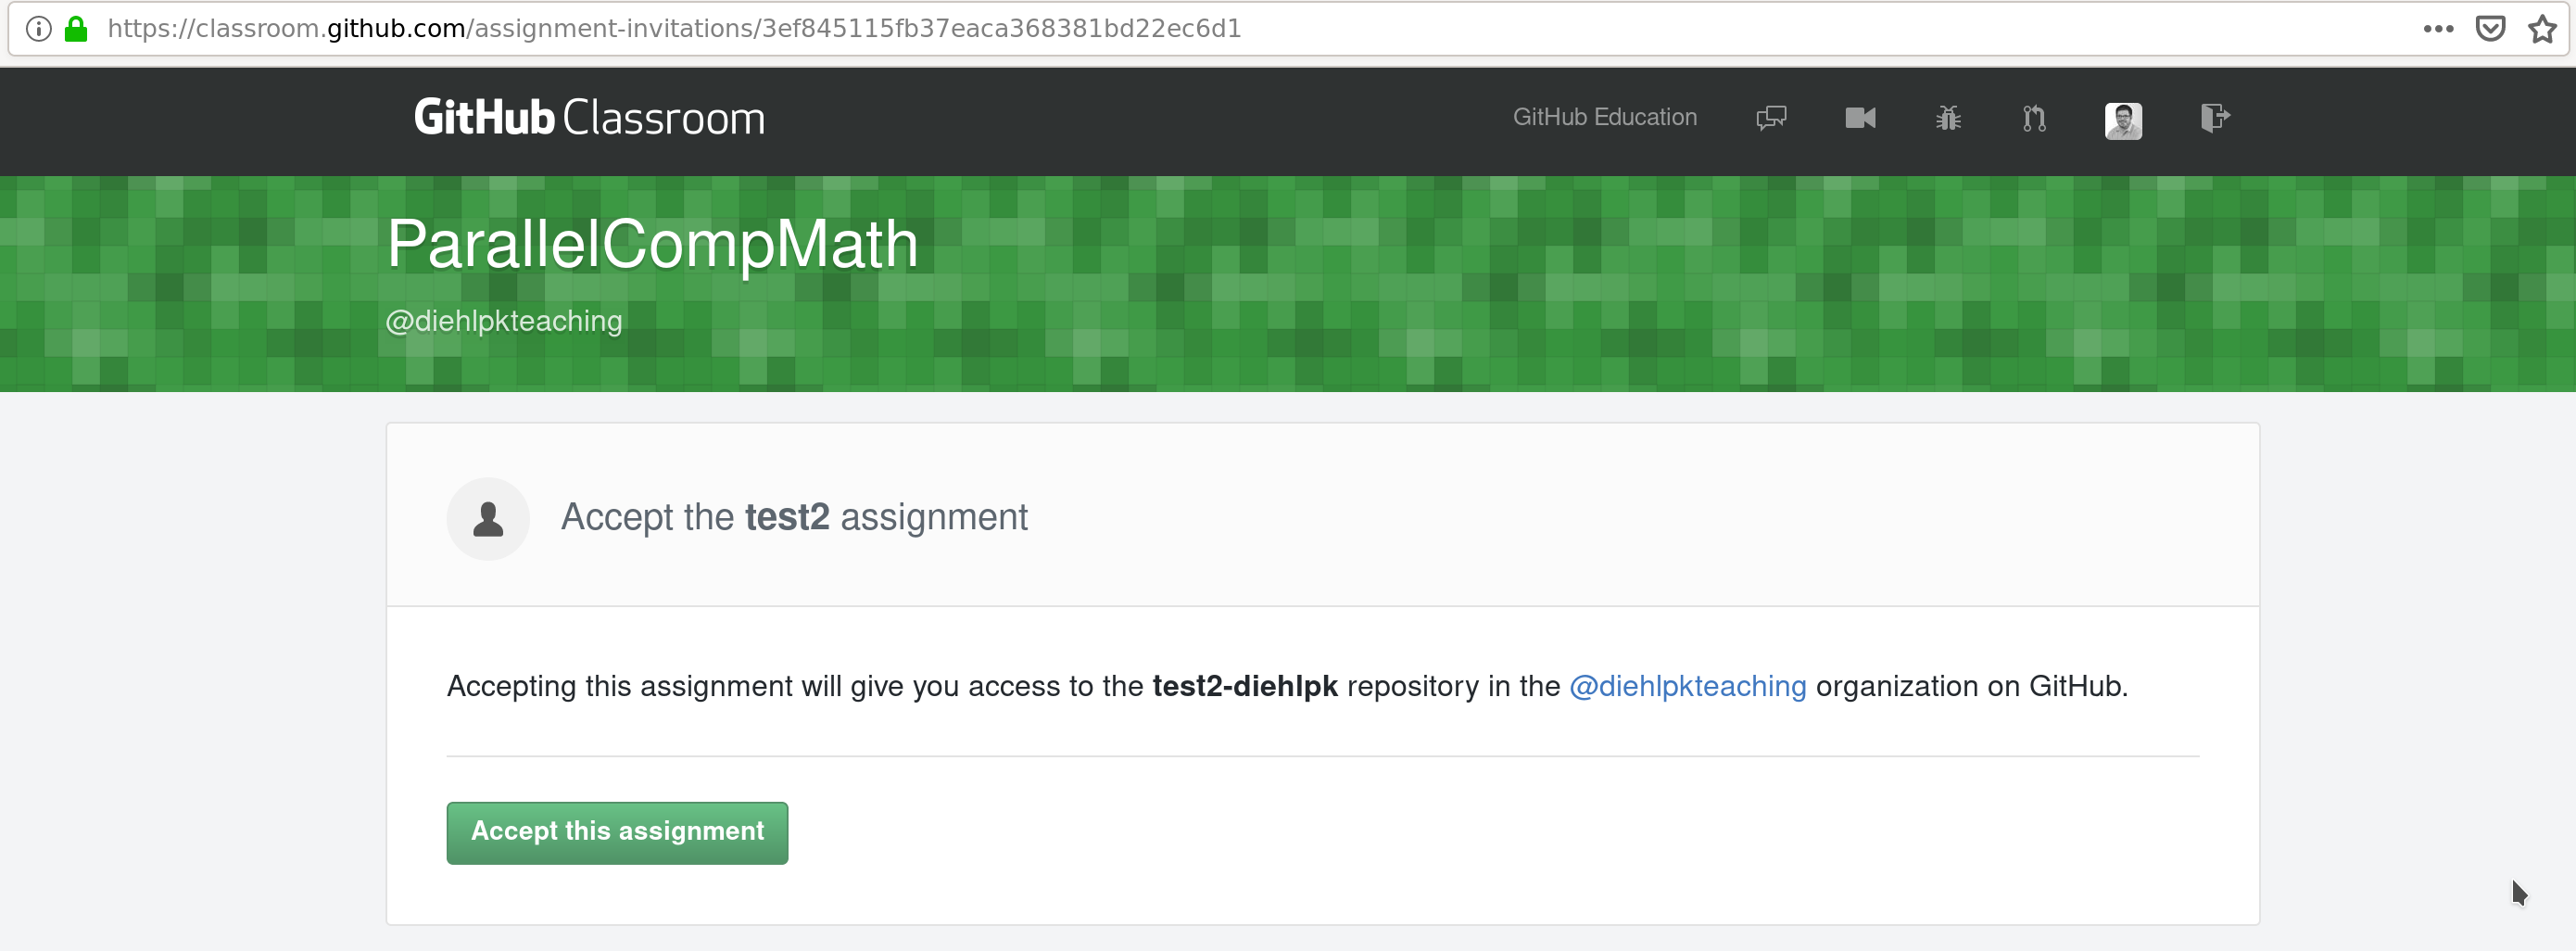
\includegraphics[width=\textwidth]{images/2019-05-17-github-assingment}
\caption{Invitation for the assignment on GitHub.}
\label{fig::github:invitation}
\end{subfigure}

\begin{subfigure}{.75\textwidth}
  \centering
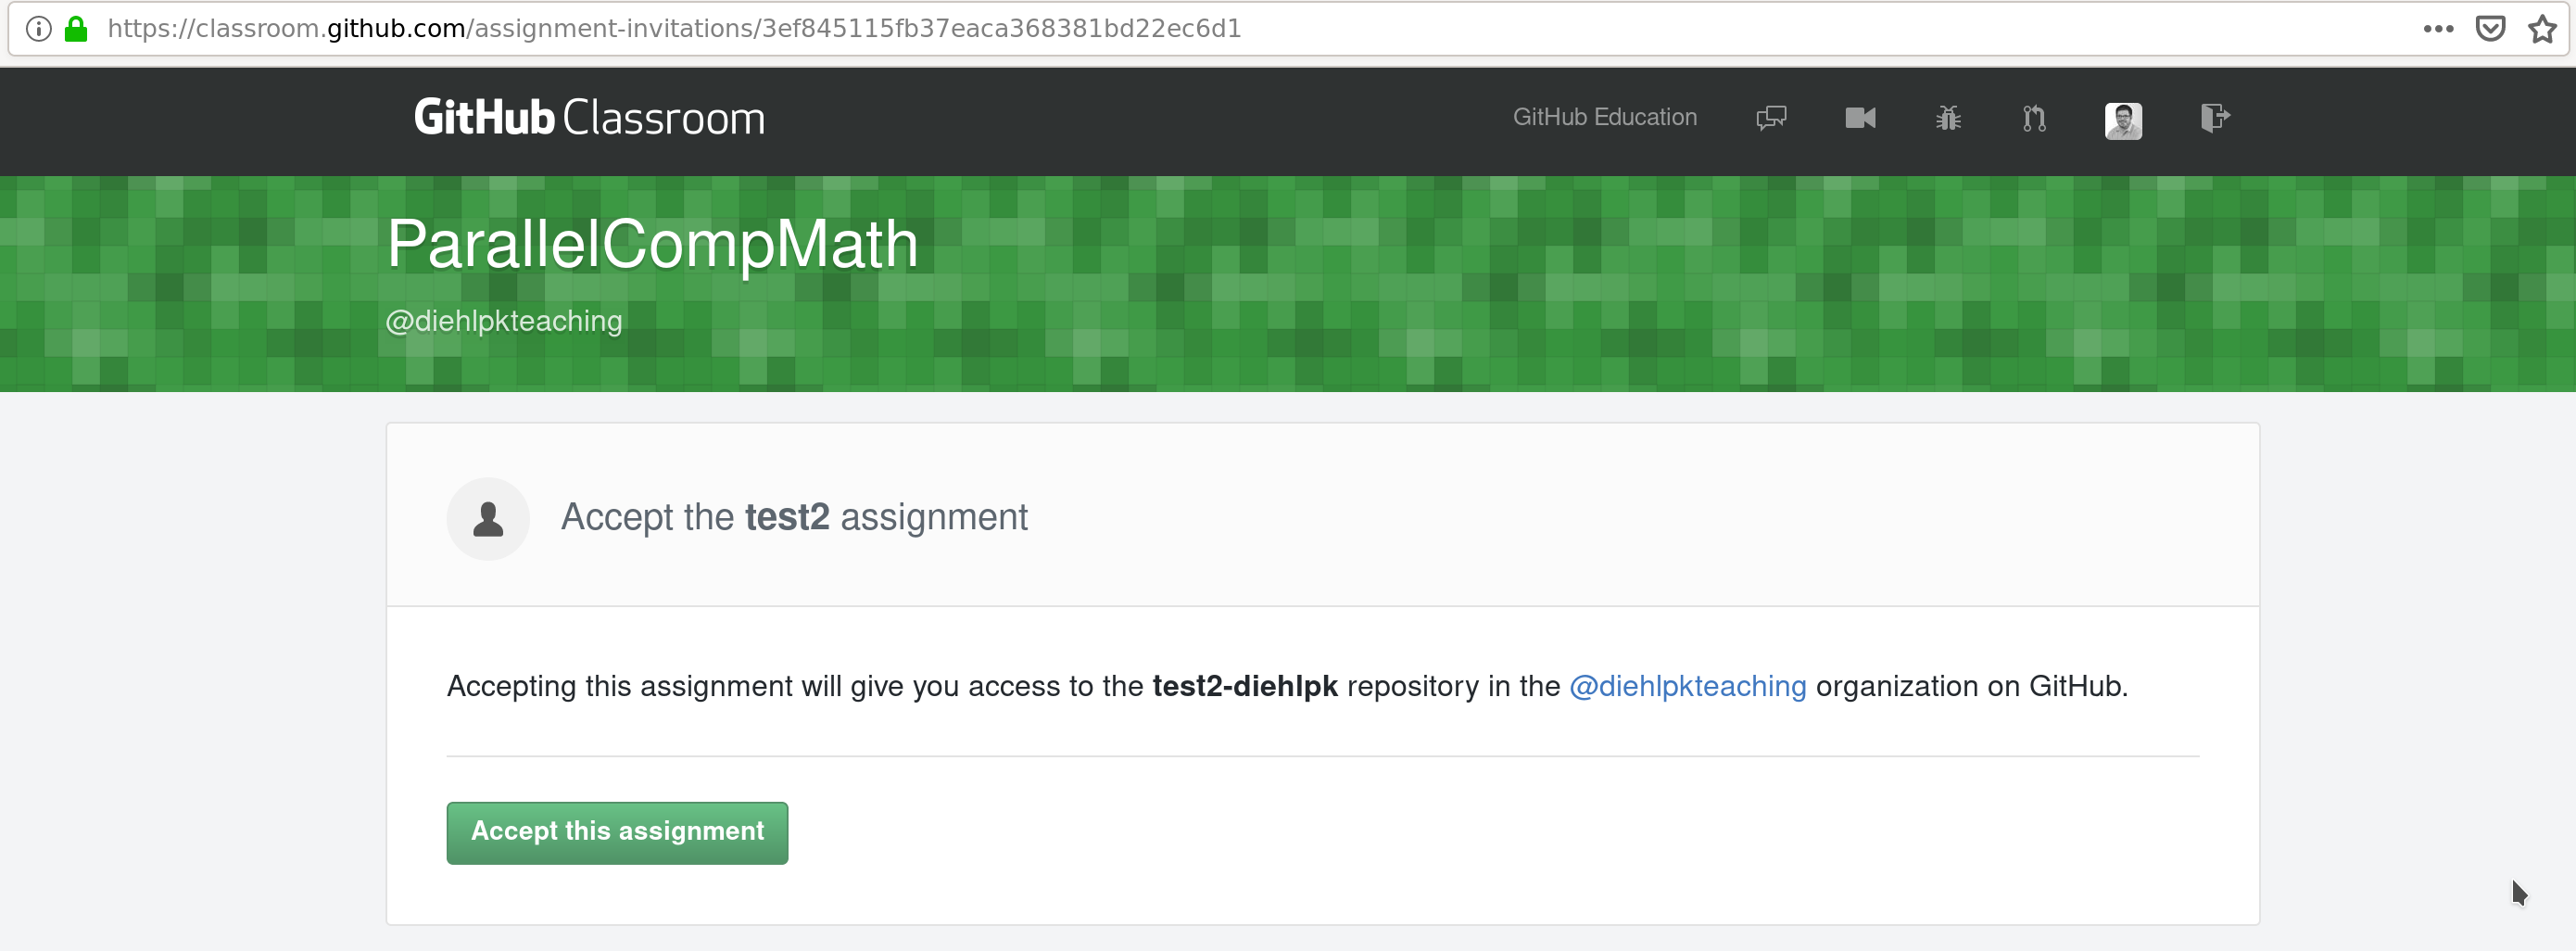
\includegraphics[width=\textwidth]{images/2019-05-17-github-assingment}
\caption{Confirmation of the acceptance and the link to submit your assignment.}
\label{fig::github:assignment}
\end{subfigure}
\caption{Accepting assignments on GitHub classroom.}
\end{figure}

\begin{lstlisting}[language=bash,caption={Setting up a ssh key\label{git:push}},float,floatplacement=tb]
git clone https://github.com/diehlpkteaching/test-diehlpk.git
cd test-diehlpk
touch exercise.cpp
git add exercise.cpp
# Work on your exercise
git commit -a
git push
\end{lstlisting}

\newpage
\theendnotes


%----------------------------------------------------------------------------------------
%	BIBLIOGRAPHY
%----------------------------------------------------------------------------------------

\chapter*{Bibliography}
\addcontentsline{toc}{chapter}{\textcolor{azure}{Bibliography}} % Add a Bibliography heading to the table of contents

%------------------------------------------------

\section*{Articles}
\addcontentsline{toc}{section}{Articles}
\printbibliography[heading=bibempty,type=article]

%------------------------------------------------

\section*{Books}
\addcontentsline{toc}{section}{Books}
\printbibliography[heading=bibempty,type=book]

%------------------------------------------------

\section*{In proceedings}
\addcontentsline{toc}{section}{In proceedings}
\printbibliography[heading=bibempty,type=inproceedings]




%----------------------------------------------------------------------------------------
%	INDEX
%----------------------------------------------------------------------------------------

\cleardoublepage % Make sure the index starts on an odd (right side) page
\phantomsection
\setlength{\columnsep}{0.75cm} % Space between the 2 columns of the index
\addcontentsline{toc}{chapter}{\textcolor{azure}{Index}} % Add an Index heading to the table of contents
\printindex % Output the index

%----------------------------------------------------------------------------------------
%	List of Listings
%----------------------------------------------------------------------------------------

\cleardoublepage % Make sure the index starts on an odd (right side) page
\phantomsection
\addcontentsline{toc}{chapter}{\textcolor{azure}{List of Listings}}
\lstlistoflistings

%----------------------------------------------------------------------------------------
%	List of Figures
%----------------------------------------------------------------------------------------

\cleardoublepage % Make sure the index starts on an odd (right side) page
\phantomsection
\addcontentsline{toc}{chapter}{\textcolor{azure}{List of Figures}}
\listoffigures

%----------------------------------------------------------------------------------------
%	List of Video lectures
%----------------------------------------------------------------------------------------

\chapter*{List of video lectures}
\addcontentsline{toc}{chapter}{\textcolor{azure}{Video lectures}}


\begin{itemize}
\item \href{https://www.youtube.com/watch?v=asGZTCR53KY&list=PL7vEgTL3FalY2eBxud1wsfz8OKvE9sd_z}{C++ Lecture 1 - The Standard Template Library}
\item \href{https://www.youtube.com/watch?v=iU3wsiJ5mts}{C++ Lecture 2 - Template Programming }
\item \href{https://www.youtube.com/watch?v=6PWUByLZO0g}{C++ Lecture 4 - Template Meta Programming}
\item \href{https://www.youtube.com/watch?v=Vck6kzWjY88}{The C++17 Parallel Algorithms Library and
Beyond}
\item \href{https://youtu.be/5vr7ItjyIH8}{Modern CUDA and C++}
\item \href{https://www.youtube.com/watch?v=Vck6kzWjY88}{The C++17 Parallel Algorithms Library and
Beyond}
\item \href{https://www.youtube.com/watch?v=js-e8xAMd1s}{The Asynchronous C++ Parallel Programming Model}
\item \href{https://www.youtube.com/watch?v=_Uv-_K3KTek&t=32s}{Nonlocality in Peridynamics}
\end{itemize}

\end{document}
